% Load the kaobook class
\documentclass[
	fontsize=10.8pt, % Base font size
	twoside=true, % Use different layouts for even and odd pages (in particular, if twoside=true, the margin column will be always on the outside)
	open=any, % If twoside=true, uncomment this to force new chapters to start on any page, not only on right (odd) pages
	secnumdepth=0, % How deep to number headings. Defaults to 1 (sections)
]{kaobook}

% Choose the language
\usepackage[english]{babel} % Load characters and hyphenation
\usepackage[english=british]{csquotes}	% English quotes

% Load packages for testing
\usepackage{blindtext}
%\usepackage{showframe} % Uncomment to show boxes around the text area, margin, header and footer
%\usepackage{showlabels} % Uncomment to output the content of \label commands to the document where they are used

% Load the bibliography package
\usepackage{kaobiblio}
\addbibresource{minimal.bib} % Bibliography file

% Load mathematical packages for theorems and related environments
\usepackage{kaotheorems}

% Load the package for hyperreferences
\usepackage{kaorefs}

\graphicspath{{images/}{./}} % Paths where images are looked for

\makeindex[columns=3, title=Alphabetical Index, intoc] % Make LaTeX produce the files required to compile the index

% ENDER

\usepackage{color}

\counterwithout{subsubsection}{subsection}
\let\theequation\thesubsection
\let\thesubsubsection\thesubsection
\makeatletter
\let\mytagform@=\tagform@
\def\tagform@#1{\maketag@@@{\color{Black}(#1)}}
\makeatother

\usepackage{hyperref}
\newcommand{\inlineeqnum}{~~\color{Black}\mbox{(\theequation)}\refstepcounter{subsection}}

\usepackage{graphicx}
\usepackage{mathbbol}
\usepackage{tikz}

\input RoyalIn.fd
\newcommand*\initfamily{\usefont{U}{RoyalIn}{xl}{n}}
\input Sanremo.fd
\newcommand*\initfamilya{\usefont{U}{Sanremo}{xl}{n}}

\usepackage{beuron}
\usepackage{cancel}
%\usepackage{mathtools}
%\usepackage{calrsfs}

\DeclareMathAlphabet{\pazocal}{OMS}{zplm}{m}{n}

% Reset sidenote counter at chapters
\counterwithin*{sidenote}{chapter}

\usepackage[bottom]{footmisc}
\raggedbottom
\begin{document}

%----------------------------------------------------------------------------------------
%	BOOK INFORMATION
%----------------------------------------------------------------------------------------

%\titlehead{Document Template}
\title[Mecánica Clásica]{{\fontsize{75pt}{0pt}\selectfont \initfamily{MECANICA
CLÁSICA}}}
\author[Abel Rosado]{\fontsize{30pt}{0pt}\selectfont \initfamilya{ABEL ROSADO} \fontsize{12pt}{0pt}\\
\url{https://github.com/EnderMk9/MyOI}}
\date{\today}
%\publishers{An Awesome Publisher}

%----------------------------------------------------------------------------------------

\frontmatter % Denotes the start of the pre-document content, uses roman numerals

%----------------------------------------------------------------------------------------
%	COPYRIGHT PAGE
%----------------------------------------------------------------------------------------

\makeatletter
\uppertitleback{\@titlehead} % Header

\lowertitleback{
	\textbf{Copyright} \\
	\ccby\ This work is licensed under a Creative Commons Attribution 4.0 International License.
	
	\medskip
	
	\textbf{Credits} \\
	This document was typeset with the help of \href{https://www.latex-project.org/}{\LaTeX} using the \href{https://github.com/fmarotta/kaobook/}{kaobook} class.
	
}
\makeatother

%----------------------------------------------------------------------------------------
%	DEDICATION
%----------------------------------------------------------------------------------------

\dedication{
	Come, let us hasten to a higher plane

	Where dyads tread the fairy fields of Venn,

	Their indices bedecked from one to n

	Commingled in an endless Markov chain!\\

	\vspace{20pt}

	In Riemann, Hilbert or in Banach space
	
	Let superscripts and subscripts go their ways
	
	Our asymptotes no longer out of phase,

	We shall encounter, counting, face to face.\\

	\vspace{20pt}

	For what did Cauchy know, or Christoffel,

	Or Fourier, or any Boole or Euler,

	Wielding their compasses, their pens and rulers,

	Of thy supernal sinusoidal spell?\\

	\vspace{20pt}

	Ellipse of bliss, converge, O lips divine!

	The product of our scalars is defined!

	Cyberiad draws nigh, and the skew mind

	Cuts capers like a happy haversine.\\

	\vspace{20pt}

	I see the eigenvalue in thine eye,

	I hear the tender tensor in thy sigh.

	Bernoulli would have been content to die,

	Had he but known such $a^2 \cos2\varphi$!
	\flushright -- Stanislaw Lem, The Cyberiad
}

%----------------------------------------------------------------------------------------
%	OUTPUT TITLE PAGE AND PREVIOUS
%----------------------------------------------------------------------------------------

% Note that \maketitle outputs the pages before here
\maketitle

%----------------------------------------------------------------------------------------
%	PREFACE
%----------------------------------------------------------------------------------------

% \chapter*{Preface}

% TO-DO

%----------------------------------------------------------------------------------------
%	TABLE OF CONTENTS & LIST OF FIGURES/TABLES
%----------------------------------------------------------------------------------------

\begingroup % Local scope for the following commands

% Define the style for the TOC, LOF, and LOT
%\setstretch{1} % Uncomment to modify line spacing in the ToC
%\hypersetup{linkcolor=blue} % Uncomment to set the colour of links in the ToC
\setlength{\textheight}{230\vscale} % Manually adjust the height of the ToC pages

% Turn on compatibility mode for the etoc package
\etocstandarddisplaystyle % "toc display" as if etoc was not loaded
\etocstandardlines % "toc lines as if etoc was not loaded

\tableofcontents % Output the table of contents

%\listoffigures % Output the list of figures

% Comment both of the following lines to have the LOF and the LOT on different pages
\let\cleardoublepage\bigskip
\let\clearpage\bigskip

%\listoftables % Output the list of tables

\endgroup

%----------------------------------------------------------------------------------------
%	MAIN BODY
%----------------------------------------------------------------------------------------

\mainmatter % Denotes the start of the main document content, resets page numbering and uses arabic numbers
\setchapterstyle{kao} % Choose the default chapter heading style

\pagelayout{wide} % No margins
\addpart[Mecánica Analítica]{\fontsize{55pt}{0pt} \setstretch{2} \textbeuron{Mecanica Analitica}}
\pagelayout{margin} % Restore margins

\chapter{Cálculo Variacional}

%-------------------------------------------------------------------------------------------
\refstepcounter{subsection}
Tenemos una función $f:\mathbcal{U}\in \mathbb{R} \mapsto f(x)\in \mathbb{R}$, donde tanto el dominio $\mathbcal{U}$ como la imagen pertencen a $\mathbb{R}$.
En contraposición, un funcional es una función $F: \mathbcal{f} \in \mathcal{F}\{x,\mathbb{R}\} \mapsto F[f]\in \mathbb{R}$, donde $\mathcal{F}\{x,\mathbb{R}\}$ es el conjunto de todas las funciones reales de una variable \sidenote[]{Aunque se puede definir un funcional como una función de $\mathcal{F}\{x,\mathbb{R}\}^n$ para $n$ funciones reales.}, tal que la imagen es un número real.

La forma genérica de los funcionales que nos interesan es la siguiente, donde ';' indica que $x$ es la variable independiente, y $f$ y $f'$ dependen explícitamente de x, y por consiguiente depende entre sí, aunque no de forma explícita en la mayoría de circunstancias:
\begin{equation}
    F[f]=\int_{x_A}^{x_B}{g(f(x),f'(x);x)dx} \label{1.0.1}
\end{equation} \refstepcounter{subsection}
Nos interesan solo las funciones $f$ tales que $f(x_A)=y_A; \ f(x_B)=y_B \label{1.0.2} \inlineeqnum$, de tal forma que la función este fija en los extremos de la integral, esta propiedad va a resultar muy importante más adelante.
    
El principal objetivo que tenemos en mente es encontrar una $f$ que extremize $F$, es decir, que $F(f)$ sea un máximo o mínimo del funcional.
%-------------------------------------------------------------------------------------------
\section{Método de pequeñas variaciones} \refstepcounter{subsection}
\begin{marginfigure}[0cm]
	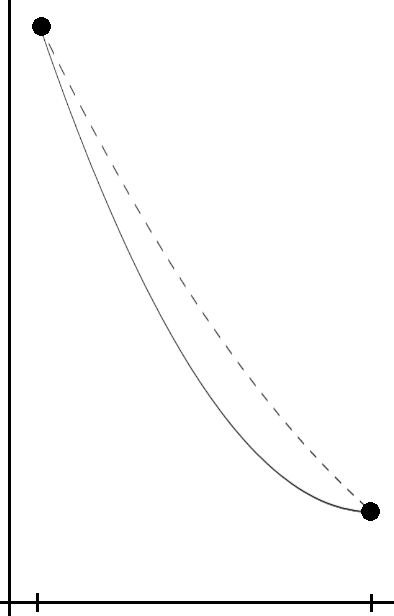
\includegraphics{1}
	\labfig{margin1}
\end{marginfigure}
Definimos $\delta y(x)\equiv\bar{y}(x)-y(x) \label{1.1.1} \inlineeqnum$, donde $\bar{y}$ es el camino variado e $y$ es el camino de referencia. Supondremos que el camino de referencia es el camino que extremiza el funcional, entonces una pequeña variación $\delta y$ no debería alterar el funcional.

Podemos parametrizar $\delta y(x) \equiv a \eta(x) \label{1.1.2} \inlineeqnum$, donde $a$ es un parámetro independiente de $x$ y $\eta(x)=\delta y(x)/a \label{1.1.2} \inlineeqnum$ es una función arbitraria que da forma el camino variado y que debe cumplir que $\eta(x_A)=\eta(x_B)=0 \label{1.1.4} \inlineeqnum$ para verificar las condiciones que hemos impuesto en (1.0.2), ya que todo camino, sea el de referencia o el variado, debe cumplirlas.

Definimos entonces una nueva función $Y(x,a)\equiv y(x)+a\eta(x) \label{1.1.5} \inlineeqnum$ tal que $Y(x,0)=y(x)$ y $Y(x,a)=\bar{y}(x)$. Si derivamos esta función con repecto a $a$, y con respecto a $x$ tenemos
\begin{equation}\label{1.1.6}
\frac{\partial Y}{\partial a}=\eta(x) ; \ \ \frac{\partial Y}{\partial x}=y'(x)+a\eta'(x)\equiv Y'(x,a); \ \  \frac{\partial Y'}{\partial a} = \eta ' (x)
\end{equation} \refstepcounter{subsection}
Podemos definir ahora $\delta y'(x) \equiv \bar{y}'(x)-y'=Y'(x,a)-Y'(x,0)$, que por la expresión anterior nos resulta $\delta y'(x)=a \eta'(x) \label{1.1.7} \inlineeqnum$.
Combinando ahora (1.1.7) y (1.1.2) podemos llegar a la conclusión de que la derivada y $\delta$ conmutan
\begin{equation}\label{1.1.8}
    \delta y'(x)=a \frac{d}{dx} \eta(x)=\frac{d}{dx}\left(a\eta(x)\right)=\frac{d}{dx} \delta y \implies \delta \left(\frac{dy}{dx}\right)=\frac{d}{dx} \delta y 
\end{equation} \refstepcounter{subsection}
%-------------------------------------------------------------------------------------------
\subsection{Variación de una función}
Si partimos de una función $g(y,y';x)$, queremos que no dependa de un solo camino sino de una familia de ellos,  definimos $\mathbb{g}(x,a)=g(Y,Y';x)$. Definimos la variación total de la función como $\Delta \mathbb{g} \equiv \mathbb{g}(Y(x,a),Y'(x,a);x)-\mathbb{g}(Y(x,0),Y'(x,0);x) \label{1.1.9} \inlineeqnum$. Como últimamente $\mathbb{g}$ depende solo de $x$ y de $a$, podemos expandir $\mathbb{g}$ por serie de Taylor de $a$
\begin{equation} \label{1.1.10}
    \mathbb{g}(x,a) = \mathbb{g}(x,0)+\left.\frac{\partial \mathbb{g}}{\partial a}\right|_{a=0} a + O(a^2)
\end{equation} \refstepcounter{subsection}
Reorganizando los términos y volviendo a añadir la dependiencia en $Y$ e $Y'$ llegamos a 
\begin{equation} \label{1.1.11}
    \overbrace{\mathbb{g}(x,a) - \mathbb{g}(x,0) }^{\Delta \mathbb{g}} = \overbrace{\left.\frac{\partial \mathbb{g}(Y(x,a),Y'(x,a);x)}{\partial a}\right|_{a=0} a}^{\delta \mathbb{g}} + O(a^2)
\end{equation} \refstepcounter{subsection}
Donde $\delta \mathbb{g}$ es la variación primera de la función, que podemos reescribir desarrollando la derivada usando la regla de la cadena, y usamos (1.1.2) y (1.1.7)
\begin{equation} \label{1.1.12}
    \delta \mathbb{g}= \left.\left[\left.\frac{\partial \mathbb{g}}{\partial Y}\right|_{Y} \frac{\partial Y}{\partial a} + \left.\frac{\partial \mathbb{g}}{\partial Y'}\right|_{Y} \frac{\partial Y'}{\partial a}\right]\right|_{a=0} a = \left.\frac{\partial \mathbb{g}}{\partial Y}\right|_{y} a \eta + \left.\frac{\partial \mathbb{g}}{\partial Y'}\right|_{y} a \eta' = \left.\frac{\partial \mathbb{g}}{\partial Y}\right|_{y} \delta y + \left.\frac{\partial \mathbb{g}}{\partial Y'}\right|_{y} \delta y'
\end{equation} \refstepcounter{subsection}
Es \textbf{muy} importante no dejar de lado las composiciones y evaluaciones resultantes de hacer Taylor y la regla de la cadena, ya que la expresión anterior nos indica que aunque $g$ dependa de cualquier camino, cuando hacemos $\delta g$, las parciales de $g$ con respecto a sus entradas $Y$ e $Y'$ hay que \textbf{evaluarlas en el camino de referencia} $y=Y(x,0)$. De esta forma podemos reesribir (1.1.12) en términos de $g$
\begin{equation} \label{1.1.12}
    \delta \mathbb{g} = \delta g = \frac{\partial g}{\partial y} \delta y + \frac{\partial g}{\partial y'} \delta y'
\end{equation} \refstepcounter{subsection}
Observamos que nos queda una expresión similar a la regla de la cadena del diferencial exacto de una función.
%-------------------------------------------------------------------------------------------
\subsection{Variación de un funcional}
De nuevo, si partimos de un funcional $F[y]$ que depende de un único camino, definimos $\mathbb{F}([y],a) = F[Y(x,a)]$ y su variación total $\Delta \mathbb{F} = \mathbb{F}([y],a)-\mathbb{F}([y],0) \label{1.1.13} \inlineeqnum$, que desarrollando la integral llegamos inmediatamente a
\begin{equation} \label{1.1.14}
    \Delta \mathbb{F} = \int_{x_A}^{x_B}{\Delta\mathbb{g}dx}=\int_{x_A}^{x_B}{\delta \mathbb{g}dx} + O(a^2)=\underbrace{\int_{x_A}^{x_B}\delta g dx}_{\delta \mathbb{F}=\delta F} + O(a^2)
\end{equation}
\newpage
\section{Extremizar un funcional} \refstepcounter{subsection}
%-------------------------------------------------------------------------------------------
Diremos que el extremo de $F$ ocurrirá cuando $\delta F = 0$, puesto que a primer orden el funcional no cambiará de valor al variar $y$.
De (1.1.13) sustuimos en (1.1.14), sacamos factor común el parámetro $a$ e integramos por partes el segundo término, tal que $ u = \partial_{y'}g$ y $ dv = \eta' dx$
\begin{equation} \label{1.2.1}
    \int_{x_A}^{x_B}{\left[\frac{\partial g}{\partial y} \eta + \frac{\partial g}{\partial y'} \eta'\right] adx} = a \left[\int_{x_A}^{x_B}{\frac{\partial g}{\partial y} \eta dx} + \left|\frac{\partial g}{\partial y'} \eta\right|_{x_A}^{x_B} -\int_{x_A}^{x_B}{\frac{d}{dx}\left(\frac{\partial g}{\partial y'}\right) \eta dx}\right]
\end{equation} \refstepcounter{subsection} 
Por (1.1.4) el segundo término es 0, juntando las integrales y usando (1.1.2)
\begin{equation} \label{1.2.2}
    \int_{x_A}^{x_B}{\left[\frac{\partial g}{\partial y} -\frac{d}{dx}\left(\frac{\partial g}{\partial y'}\right) \right] \delta y dx}=0
\end{equation} \refstepcounter{subsection} 
Ahora, $\delta y$ es completamente arbitrario, pues depende de un parámetro independiente $a$ y de una función $\eta$ que es también arbitraria, esto es lema fundamental del Cálculo Variacional, y garantiza que si la integral debe valer 0, el primer factor debe valer siempre 0, y concluimos

\vspace{-20pt}
\Large\begin{equation} \label{1.2.3}
    \boxed{\frac{\partial g}{\partial y} -\frac{d}{dx}\left(\frac{\partial g}{\partial y'}\right) =0} \iff \delta F =0
\end{equation} \refstepcounter{subsection}\normalsize
Esta es la ecuación de \textit{Euler-Lagrange}, una ecuación diferencial en derivadas parciales de segundo orden cuya solución $y$ extremiza el funcional definido por $g$.

Es importante notar que si definimos
\begin{equation} \label{1.2.2}
    \tilde{g}(f(x),f'(x);x) = g(f(x),f'(x);x) + \frac{d}{dx} h(f(x),x)
\end{equation} \refstepcounter{subsection}
Entonces el funcional nos queda, aplicando el teorema fundamental del cálculo
\begin{equation} \label{1.2.2}
    \tilde{F}[f]=\int_{x_A}^{x_B}{\tilde{g}(f(x),f'(x);x)dx}=F[f] +\int_{x_A}^{x_B}{\frac{d}{dx} h(f(x),x) dx} = F[f] + h(f(x),x)|_{x_A}^{x_B}
\end{equation} \refstepcounter{subsection}
Y como los dos últimos términos son constantes, se verifica que $\delta \tilde{F} = \delta F$, y por lo tanto (1.2.3) permanece invariante bajo esta transformación.
%-------------------------------------------------------------------------------------------
\subsubsection{Geodésica del plano}
Un ejemplo para aplicar (1.2.3) es minimizar la distancia $d=\int{ds}$ en el plano ecuclídeo. Si $y=y(x)$, entonces $ds=\sqrt{dx^2+dy^2}=\sqrt{1+y'^2}dx=g dx$, tal que
\[\frac{\partial g}{\partial y}=0 \implies \frac{d}{dx}\left(\frac{\partial g}{\partial y'}\right)=0 \implies \frac{\partial g}{\partial y'} = \frac{y'}{\sqrt{1+y'^2}}= K \rightarrow y' = \frac{K}{\sqrt{1-K^2}}=\alpha\]
Lo cual implica que $y=\alpha x + y_0$, la ecuación de una recta.
%-------------------------------------------------------------------------------------------
\newpage
\subsection{Identidad de Beltrami}
Podemos reescribir (1.2.3) de otra forma que nos va resultar últil para resolver algunos problemas y va a resultar muy importante en episodios posteriores al definir el \textit{Hamiltoniano}
\[\frac{dg}{dx} = \frac{\partial g}{\partial y} y' + \frac{\partial g}{\partial y'}y'' + \frac{\partial g}{\partial x}\rightarrow \frac{\partial g}{\partial y} y' = \frac{dg}{dx} - \frac{\partial g}{\partial y'}y'' - \frac{\partial g}{\partial x}\]
Podemos observar que el término en el primer miembro de la segunda expresión aparece en (1.2.3) sin multiplicar por $y'$.
\[\frac{dg}{dx} - \frac{\partial g}{\partial x} - \left[\frac{\partial g}{\partial y'}y'' + y' \frac{d}{dx}\left(\frac{\partial g}{\partial y'}\right)\right]=0 \rightarrow \frac{dg}{dx} - \frac{\partial g}{\partial x} - \frac{d}{dx}\left(\frac{\partial g}{\partial y'}y'\right)=0\]
Observando que lo de dentro del paréntesis de la primera expresión es la derivada de un producto, usamos la linearidad de la derivada para obtener
\begin{equation} \label{1.3.4}
    \frac{d}{dx}\left(g -\frac{\partial g}{\partial y'}y'\right)=\frac{\partial g}{\partial x}
\end{equation}
%-------------------------------------------------------------------------------------------

\section{Generalización a varias variables} \refstepcounter{subsection} 
Denotamos $\{f_\alpha(x)\}$ a un conjunto de $N$ funciones distintas, que verifican una expresión similar a (1.0.2), $f_\alpha(x_A)=f_{\alpha A}; \ f_\alpha(x_B)=f_{\alpha B} \label{1.3.1} \inlineeqnum$.
%\sidenote{Si existe una función que las relacione, se trata de una ligadura, veáse el apartado siguiente}
Definimos entonces el siguiente funcional que depende de $\{f_\alpha\}$
\[F[\{f_\alpha\}]=\int_{x_A}^{x_B}{g(\{f_\alpha,f'_\alpha\};x)dx}\]
Ahora siguiendo un desarrollo idéntico a (1.1.12), desarrollando la regla de la cadena para cada una de las variables de $g$ resulta en un sumatorio y los argumentos siguientes para llegar a $\delta g$ son idénticos puesto que son lineales, de tal forma llegamos a la siguiente expresión
\begin{equation} \label{1.3.2}
    \delta g = \sum{\frac{\partial g}{\partial f_\alpha} \delta f_\alpha + \frac{\partial g}{\partial f'_\alpha} \delta f'_\alpha}
\end{equation} \refstepcounter{subsection} 
La expresión (1.1.15) no dependía de las variables de $g$, por lo que es directamente aplicable, sustituyendo (1.3.2) y haciendo la regla de la cadena igual que en (1.2.1) llegamos a una expresión similar a (1.2.2), usando que la integral conmuta con el sumatorio
\begin{equation} \label{1.3.3}
    \delta F = \sum \int_{x_A}^{x_B}{\left[\frac{\partial g}{\partial f_\alpha} -\frac{d}{dx}\left(\frac{\partial g}{\partial f'_\alpha}\right) \right] \delta f_\alpha dx}=0
\end{equation} \refstepcounter{subsection} 
Para poder concluir que cada sumando es 0, y que entonces por ser $\delta f_\alpha$ arbitraria cada término en corchetes es 0, es necesario que los $\delta f_\alpha$ sean independientes entre sí, que es equivalente a que no exista una dependencia explícita entre los $f_\alpha(x)$, que podria estar por ejemplo expresada por una ecuación relacionando varias de ellas. Si se cumple que son independientes, entonces

\vspace{-20pt}
\Large\begin{equation} \label{1.3.3}
    \boxed{\frac{\partial g}{\partial f_\alpha} -\frac{d}{dx}\left(\frac{\partial g}{\partial f'_\alpha}\right) =0} \iff \delta F =0
\end{equation} \refstepcounter{subsection}\normalsize
Ahora tenemos un sistema de ecuaciones de \textit{Euler-Lagrange} cuyas soluciones $f_\alpha(x)$ extremizan el funcional.
%-------------------------------------------------------------------------------------------
\subsection{Ligaduras}
En el caso de que existan $m$ ecuaciones de ligadura de la forma $G_i(\{f_\alpha\};t)=0$, tenemos dos opciones, la primera es resolver el sistema de ecuaciones que forman expresando $m$ funciones como dependientes de las otras $N-m$ funciones restantes, y aplicar (1.3.4) a las $N-m$ funciones independientes.

En el caso de que esto no sea posible resolver el sistema, debemos recurrir a multiplicadores de \textit{Lagrange}.
%-------------------------------------------------------------------------------------------
\subsubsection{Multiplicadores de Lagrange}
Partimos de que tenemos $m$ ecuaciones $G_i(\{f_\alpha\};x)=0$ que no sabemos resolver, $\Delta G_i =0$, es decir, $G_i$ se aplica de la misma forma tanto a los caminos de referencia como a los variados, además $\Delta G_i = \delta G_i + O(a^2) = 0$, como $a$ es arbitrario, entonces $\delta G_i =0$. Aplicando la regla de la cadena de (1.1.13)
\begin{equation} \label{1.3.5}
    \delta G_i(\{f_\alpha\};x) = \sum_\alpha^N{\frac{\partial G_i}{\partial f_\alpha} \delta f_\alpha}=\sum_\alpha^N{a_{i\alpha} \delta f_\alpha}=0; \ \ \ a_{i\alpha} = \frac{\partial G_i}{\partial f_\alpha}
\end{equation} \refstepcounter{subsection}
Así tenemos la ecuación que nos relaciona las distintas $\delta f_\alpha$, el término de la derivada lo podemos expresar como las componentes de un matriz. Podemos separar la expresión anterior tal que
\begin{equation} \label{1.3.6}
    \delta G_i= \sum_{\gamma=1}^{N-m}{a_{i\gamma} \delta f_\gamma} + \sum_{\beta=N-m+1}^{N}{a_{i\beta} \delta f_\beta} = 0
\end{equation} \refstepcounter{subsection}
La matriz del segundo término es cuadrada $(m\times m)$, y es una matriz jacobiana cuyo determinante va a ser no nulo si las ecuaciones de ligadura son independientes entre sí, de lo contrario algunas sobran. Esto implica que esa matriz tiene inversa, expresando (1.3.6) como operaciones matriciales ($N-m < \beta \leq N$)
\begin{equation} \label{1.3.7}
    0= A\mathbf{x} + J\mathbf{y} \implies \mathbf{y}=-J^{-1}A\mathbf{x}; \ \ \delta f_\beta = -\sum_{a=1}^m{\sum_{\gamma =1}^{N-m}{J^{-1}_{\beta a}a_{a\gamma}\delta f_\gamma}}
\end{equation} \refstepcounter{subsection}
De esta forma, hemos encontrado la dependencia explícita de $\delta f_\beta$ en función de los $\delta f_\gamma$, estos últimos siendo independientes entre sí. Ahora tomamos (1.3.3) y renombramos el factor en corchetes por $\Gamma_\alpha$ y separamos como en (1.3.6)
\begin{equation} \label{1.3.8}
    0 = \delta F = \int_{x_A}^{x_B}{\sum_\alpha^N{(\Gamma_\alpha \delta f_\alpha)}dx=\int_{x_A}^{x_B}{\sum_{\gamma =1}^{N-m}{(\Gamma_\gamma \delta f_\gamma)}dx+\int_{x_A}^{x_B}{\sum_{\beta=N-m+1}^{N}{(\Gamma_\beta \delta f_\beta)}dx}}}
\end{equation} \refstepcounter{subsection}
Sustituyendo $\delta f_\beta$ de (1.3.7)
\begin{equation} \label{1.3.9}
    0 =\int_{x_A}^{x_B}{\sum_{\gamma =1}^{N-m}{(\Gamma_\gamma \delta f_\gamma)}dx-\int_{x_A}^{x_B}{\sum_{\beta=N-m+1}^{N}{\left(\Gamma_\beta \sum_{a=1}^m{\sum_{\gamma =1}^{N-m}{J^{-1}_{\beta a}a_{a\gamma}\delta f_\gamma}}\right)}dx}}
\end{equation} \refstepcounter{subsection}
Como los sumatorios conmutan podemos llegar a
\begin{equation} \label{1.3.10}
    0  =\int_{x_A}^{x_B}{\sum_{\gamma =1}^{N-m}{(\Gamma_\gamma \delta f_\gamma)}dx-\int_{x_A}^{x_B}\sum_{\gamma =1}^{N-m}{{\sum_{a=1}^m{\sum_{\beta=N-m+1}^{N}{\Gamma_\beta J^{-1}_{\beta a}a_{a\gamma}\delta f_\gamma}}}dx}}
\end{equation} \refstepcounter{subsection} 
Y ahora podemos unificar los sumatorios de $\gamma$ y sacar factor común $\delta f_\gamma$
\begin{equation} \label{1.3.11}
    0  =\int_{x_A}^{x_B}{\sum_{\gamma =1}^{N-m}{\delta f_\gamma \left(\Gamma_\gamma -{\sum_{a=1}^m{\sum_{\beta=N-m+1}^{N}{\Gamma_\beta J^{-1}_{\beta a}a_{a\gamma}}}}\right)} dx}
\end{equation} \refstepcounter{subsection} 
Definimos entonces $\lambda_a=\sum_{\beta=N-m+1}^{N}{\Gamma_\beta J^{-1}_{\beta a}}$ como los multiplicadores de \textit{Lagrange} y reemplazando $a_{a\gamma}$ por su definición de (1.3.5)
\begin{equation} \label{1.3.12}
    0  =\int_{x_A}^{x_B}{\sum_{\gamma =1}^{N-m}{\delta f_\gamma \left(\Gamma_\gamma -{\sum_{a=1}^m{\lambda_a \frac{\partial G_a}{\partial f_\gamma}}}\right)} dx}
\end{equation} \refstepcounter{subsection}
Ahora como $\delta f_\gamma$ son independientes entre sí, podemos aplicar el mismo argumento que en los otros casos y concluir que lo del paréntesis debe ser igual a 0 para todos los $\gamma$, tal que ($1 \leq \gamma \leq N-m$)
\begin{equation} \label{1.3.13}
    \Gamma_\gamma -{\sum_{a=1}^m{\lambda_a \frac{\partial G_a}{\partial f_\gamma}}}=0
\end{equation} \refstepcounter{subsection}
Podemos ahora comprobar que si $N-m < \gamma \leq N$
\[\Gamma_\gamma -{\sum_{a=1}^m{\lambda_a \frac{\partial G_a}{\partial f_\gamma}}}\right)=\Gamma_\gamma -{\sum_{a=1}^m{\lambda_a J_{a\gamma}}}\right) = \Gamma_\gamma -{\sum_{a=1}^m{\sum_{\beta=N-m+1}^{N}{\Gamma_\beta J^{-1}_{\beta a}} J_{a\gamma}}}=\]
\begin{equation} \label{1.3.14}
    =\Gamma_\gamma -\sum_{\beta=N-m+1}^{N}{\Gamma_\beta \delta_{\beta \gamma}} \right) = \Gamma_\gamma - \Gamma_\gamma = 0
\end{equation} \refstepcounter{subsection}
También se verifica (1.3.12), por lo que entonces
\Large\begin{equation} \label{1.3.15}
    \boxed{\frac{\partial g}{\partial f_\alpha} -\frac{d}{dx}\left(\frac{\partial g}{\partial f'_\alpha}\right) ={\sum_{i=1}^m{\lambda_i \frac{\partial G_i}{\partial f_\alpha}}} \ \ \ \ \ G_i(\{f_\alpha\}) = 0}
\end{equation} \refstepcounter{subsection}\normalsize
Tenemos por lo tanto un sistema de $N+m$ ecuaciones, que incluye las ecuaciones de \textit{Euler-Lagrange} modificadas y las ecuaciones de ligadura, y las incognitas son las $f_\alpha$ y las $\lambda_i$.
\chapter{Mecánica Lagrangiana}
\labch{intro}
%-------------------------------------------------------------------------------------------
Ahora la variable independiente sobre la que vamos a trabajar va a ser el tiempo, $t$, y las variables dependientes son las coordenadas cartesianas $\{x_{\alpha i}\}$, donde $\alpha$ indica la partícula y $i$ indica la componente de la posición.
Definimos además las derivadas totales temporales como $\{\dot{x}_{\alpha i}\}$.

\section{Principio de Hamilton}\refstepcounter{subsection}

Definimos una función llamada \textbf{Lagrangiano}\sidenote{La definición de \textbf{Lagrangiano} dependerá de la configuración del sistema físico, pero como norma géneral en mecánica clásica (2.1.1) es la expresión más común de la función que verifica (2.1.3). Esto se demuestra más adelante.}
\begin{equation} \label{2.1.1}
    \pazocal{L}(\{x_{\alpha i},\dot{x}_{\alpha i}\};t)=T-U
\end{equation} \refstepcounter{subsection}
Dónde $T$ es la energía cinética del sistema y $U$ es la energía potencial (conservativa o no), de tal forma que definimos el siguiente funcional llamado \textbf{acción}
\begin{equation} \label{2.1.2}
    S \equiv \int_{t_A}^{t_B}{\pazocal{L}(\{x_{\alpha i},\dot{x}_{\alpha i}\};t)dt}
\end{equation} \refstepcounter{subsection}
\textbf{Principio de Hamilton o de mínima acción.} La evolución temporal de un sistema físico es aquella que extremiza la acción, es decir que $\delta S = 0$ para la evolución real del sistema, lo cual es equivalente a
\begin{equation} \label{2.1.3}
    \frac{\partial \pazocal{L}}{\partial x_{\alpha i}} -\frac{d}{dt}\left(\frac{\partial \pazocal{L}}{\partial \dot{x}_{\alpha i}}\right) =0
\end{equation} \refstepcounter{subsection}
Para la mecánica clásica, este principio es equivalente a las leyes de \textit{Newton}, cuando $\pazocal{L}$ toma la forma de (2.1.1) con ligeras modificaciones que discutiremos en las próximas secciones.
%-------------------------------------------------------------------------------------------
\subsubsection{Muelle elástico}
Un sencillo ejemplo para aplicar este principio es el de un muelle elástico en una dirección, donde $T=m\dot{x}^2/2$ y $U = kx^2/2$ (el término $mgh$ es constante y puede ser ignorado), si $\pazocal{L} = T-U$, entonces
\[\frac{\partial \pazocal{L}}{\partial x}=-kx \ \ \ \ \frac{\partial \pazocal{L}}{\partial \dot{x}}=m\dot{x} = p \ \ \ \ \frac{d p}{dt} = m\ddot{x} \rightarrow m\ddot{x} = -kx \iff F=-kx=ma\]
%-------------------------------------------------------------------------------------------
\section{Coordendas generalizadas} \refstepcounter{subsection}
Podemos realizar un cambio de variables para poder expresar $x_{\alpha i}$ en función de otras variables $q_j$, las cuales pueden resultarnos más sencillas para resolver un problema, tal que $x_{\alpha i}=x_{\alpha i}(\{q_j\};t)$. Esta transformación será invertible cuando
\vspace{-10pt}
\[J_l^k=\frac{\partial x_k}{\partial q_l}\]
el determinante de esa matriz, el jacobiano, sea no nulo, tal que existe la transformación $q_j = q_j(\{x_{\alpha i}\};t)$.

Usando la regla de la cadena podemos ver la dependencia de las velociades entre sí, $\dot{x}_{\alpha i}=\dot{x}_{\alpha i}(\{q_j,\dot{q}_j\};t)$ y que $\dot{q}_j = \dot{q}_j(\{x_{\alpha i},\dot{x}_{\alpha i}\};t)$.

De esta forma, podemos expresar $\pazocal{L}$ en función de las coordenadas y velocidades generalizadas, tal que $\pazocal{L}=\pazocal{L}(\{q_j,\dot{q}_j\};t)$ de tal forma que (2.1.3) queda como 

\vspace{-10pt}
\Large\begin{equation} \label{2.2.1}
    \boxed{\frac{\partial \pazocal{L}}{\partial q_j} -\frac{d}{dt}\left(\frac{\partial \pazocal{L}}{\partial \dot{q}_j}\right) =0}
\end{equation} \refstepcounter{subsection}\normalsize

Definimos además el \textbf{momento generalizado}, que para cartesianas es el momento lineal y para polares es el momento angular. También definimos la \textbf{fuerza generalizada}, que es la proyección del vector cartesiano en el sistema de vectores asociado a las coordenadas generalizadas.
\begin{equation} \label{2.2.2}
    p_j = \frac{\partial \pazocal{L}}{\partial \dot{q}_j} \ \ \ \ Q_j = -\frac{\partial U}{\partial q_j}=\sum_\alpha^N{\mathbf{F}_\alpha\cdot \frac{\partial \mathbf{r}_{\alpha}}{\partial q_j}}
\end{equation} \refstepcounter{subsection}
%-------------------------------------------------------------------------------------------
\section{Ligaduras}\refstepcounter{subsection}
Al igual que en la sección \textit{Ligaduras} de la sección 1.3, tendremos $M$ ecuaciones de ligadura, los tipos de las cuales se datallarán a continuación, pero antes definimos lo que vamos a denominar \textbf{grados de libertad}, que indica el número mínimo de parámetros que es necesario para especifcar la configuración del sistema en un tiempo dado, tal que $s = N\cdot d- M \label{2.3.1} \inlineeqnum$, donde $s$ son los \textbf{grados de libertad}, $N$ el número de partículas del sistema, y $d$ la dimensión del espacio.
%-------------------------------------------------------------------------------------------
\subsubsection{Tipos de ligaduras}
Cuando las ecuaciones de ligadura no dependen de las veclocidades, $G_i(\{q_j\})=0$, se denominan ligaduras \textbf{holónomas} y son con las que vamos a trabajar. Si las ecuaciones de ligadura dependen de la velocidad,$ G_i(\{q_j,\dot{q}_j\})=0$, se denominan \textbf{no holónomas} y salvo que sean integrables no trabjaremos con ellas. Son \textbf{integrables} cuando son de la forma siguiente donde $h=h(\{q_i\};t)$ tal que
\begin{equation} \label{2.3.2}
    \sum_j^{N\cdot d}{A_j(\{q_i\};t)\dot{q}_j} + B(\{q_i\};t)=0; \ \ \ \ A_j=\frac{\partial h}{\partial q_j}; \ \ \ \ B_j=\frac{\partial h}{\partial t}
\end{equation} \refstepcounter{subsection}
Entonces podemos ver que nos queda la regla de la cadena e integramos
\begin{equation} \label{2.3.3}
    \sum_j^{N\cdot d}{\frac{\partial h}{\partial q_j}\dot{q}_j} + \frac{\partial h}{\partial t}=\frac{d h}{dt} =0 \iff h(\{q_i\};t) - C = 0 \mbox{ (Holónoma)}
\end{equation} \refstepcounter{subsection}
Luego a parte si la ligadura depende explícitamente del tiempo se llama \textbf{forzada} o \textbf{reónoma}, si no depende explcítamente del tiempo, se denominan \textbf{naturales} o \textbf{esclerónomas}.
%-------------------------------------------------------------------------------------------
\subsection{Sistema holonómico}
Decimos que un sistema es \textbf{holonómico} cuando podemos resolver (o bien en cartesianas o en generalizadas) las ecuaciones de ligadura (holónomas) y expresar $m$ coordenadas como explícitamente dependientes de $s$ coordenadas independientes, reduciendo el sistema a $s$ variables que podemos resolver usando (2.2.1)  (\textit{E-L}).
%-------------------------------------------------------------------------------------------
\subsection{Multiplicadores de Lagrange}
En el caso en el que el sistema no sea holonómico, y no podamos resolver las ecuaciones de ligadura, al igual que en la sección 1.3 tenemos que recurrir a multiplicadores de multiplicadores de \textit{Lagrange}, podemos obtener una expresión equivalente a (1.3.15) modificando el lagrangiano de la siguiente forma
\begin{equation} \label{2.3.4}
    \pazocal{L}^* = \pazocal{L}+\sum^m{\lambda_i G_i}
\end{equation} \refstepcounter{subsection}
Que aplicando las ecuaciones de \textit{Euler-Lagrange} tanto para $q_j$ como para $\lambda_i$ resulta

\vspace{-10pt}
\Large\begin{equation} \label{2.3.5}
    \frac{\partial \pazocal{L}}{\partial q_j} -\frac{d}{dt}\left(\frac{\partial \pazocal{L}}{\partial \dot{q}_j}\right) +\underbrace{\sum^m\lambda_i(t)\frac{\partial G_i}{\partial q_j}}_{Q^L_j}=0
\end{equation} \refstepcounter{subsection}\normalsize
Donde $Q^L_j$ es la componente $j$ de la fuerza generalizada de ligadura total, que cumplen que $dW^L = \mathbf{F}^L\cdot d\mathbf{r}=0$ son fuerzas que o siempre perpendiculares a la ligadura, o que provocan que $d\mathbf{r}=0 \iff \mathbf{v}=0$ en el punto de contacto.

\section{Principio de D'Alambert}\refstepcounter{subsection}
\subsubsection{Estático}
Vamos a suponer que tenemos un sistema en equilibrio, es decir $\mathbf{F}_i = 0$ para cada partícula del sistema, o en general para cualquier punto donde se aplica una fuerza, de tal forma que $\mathbf{F}_i \cdot \delta \mathbf{r}_i = 0$.

$\delta \mathbf{r}_i$ es lo que se denomina desplazamiento virtual, el sistema no se mueve, sigue en el equilibrio, estos desplazamientos se definen respetando las ligaduras del sistema, por ejemplo, tenemos en un péndulo que por la gravedad y otra fuerza externa se encuentra en equilibrio, podemos expresar la posición en términos de las coordenadas generalizadas, que respetan las ligaduras, tal que $\mathbf{r} = l (\sin \theta \mathbf{e}_x + \cos \theta \mathbf{e}_y)$, y entonces $\delta \mathbf{r} = l (\cos \theta \mathbf{e}_x-\sin\theta \mathbf{e}_y) \delta \theta$.

Para sistemas tendremos entones $\sum_i \mathbf{F}_i \cdot \delta \mathbf{r}_i = 0$, pero esto no nos dice nada, sin embargo, podemos descomponer la fuerza total que se ejerce en un punto o partícula en fuerzas de ligadura o normal y fuerzas externas o aplicadas, tal que $\mathbf{F}_i = \mathbf{F}_i^{(a)}+\mathbf{f}_i$, aunque no es siempre facil distinguirlo a simple vista. De esta forma nos queda
\begin{equation} \label{2.1.1}
    \sum_i \mathbf{F}_i^{(a)} \cdot \delta \mathbf{r}_i + \sum_i \mathbf{f}_i \cdot \delta \mathbf{r}_i = 0
\end{equation} \refstepcounter{subsection}
Ahora, salvo casos muy extraños de ligaduras, el trabajo virtual de una fuerza normal o de ligadura se anula, como se ha explicado en el apartado anterior, de esta forma llegamos al principio de D'Alambert estático
\begin{equation} \label{2.1.1}
    \sum_i \mathbf{F}_i^{(a)} \cdot \delta \mathbf{r}_i = 0
\end{equation} \refstepcounter{subsection}
También es llamado principio del trabajo virtual, y al aplicarlo, las componentes $\delta \mathbf{r}_i$ son no nulas, en general implica que $\delta q_i \neq 0$, donde $q_i$ son las coordenadas generalizadas, por ejemplo, $\delta \theta$ en el ejemplo anterior.
\subsubsection{Dinámico}
Ahora consideraremos un sistema que no esta en equilibrio, tenemos que $\mathbf{F}_i = \dot{\mathbf{p}}_i = m_i \ddot{\mathbf{r}}_i$, de tal forma que haciendo exactamente las mismas manipulaciones que antes, y descomponiendo la fuerza total, llegamos a la versión dinámica del principio de D'Alambert
\begin{equation} \label{2.1.1}
    \sum_i (\dot{\mathbf{p}}_i-\mathbf{F}_i^{(a)}) \cdot \delta \mathbf{r}_i = 0
\end{equation} \refstepcounter{subsection}
\subsubsection{Lagrangiano}
Si hacemos el cambio a coordenadas generalizadas usando la regla de la cadena, tenemos
\begin{equation} \label{2.1.1}
    \delta \mathbf{r}_i = \sum_j \frac{\partial \mathbf{r}_i}{\partial q_j} \delta q_j
\end{equation} \refstepcounter{subsection}
Podemos ahora definir de nuevo la fuerza generalizada
\begin{equation} \label{2.1.1}
    \sum_i \mathbf{F}_i \cdot \delta \mathbf{r}_i = \sum_{ij} \mathbf{F}_i \cdot \frac{\partial \mathbf{r}_i}{\partial q_j} \delta q_j = \sum_j Q_j \delta q_j \implies Q_j = \sum_i \mathbf{F}_i \cdot \frac{\partial \mathbf{r}_i}{\partial q_j}
\end{equation} \refstepcounter{subsection}
Es importante notar que $Q_j$ no tiene unidades de fuerza en general, pero $Q_j \delta q_j$ siempre tiene unidades de trabajo. Si consideramos solo fuerzas conservativas (aunque pueden depender del tiempo) tenemos
\begin{equation} \label{2.1.1}
    \mathbf{F}_i = -\nabla_i U \ \ \ \ \ \ Q_j = -\sum_i \nabla_i U \cdot \frac{\partial \mathbf{r}_i}{\partial q_j} = - \sum_{ik} \frac{\partial U}{\partial r_{ik}} \frac{\partial r_{ik}}{\partial q_j} = - \frac{\partial U}{\partial q_j}
\end{equation} \refstepcounter{subsection}
Ahora, hacemos lo mismo pero con el otro término de (2.4.3), y descomponemos una regla del producto
\begin{equation} \label{2.1.1}
    \sum_i \dot{\mathbf{p}}_i \cdot \delta \mathbf{r}_i = \sum_{ij} m \ddot{\mathbf{r}}_i \cdot \frac{\partial \mathbf{r}_i}{\partial q_j} \delta q_j \ \ \ \ \ \ \ \sum_{i} m \ddot{\mathbf{r}}_i \cdot \frac{\partial \mathbf{r}_i}{\partial q_j} = \sum_i \left[ \frac{d}{dt}\left(m_i \dot{\mathbf{r}}_i \cdot \frac{\partial \mathbf{r}_i}{\partial q_j}\right)- m_i \dot{\mathbf{r}}_i\frac{d}{dt}\left(\frac{\partial \mathbf{r}_i}{\partial q_j}\right)\right]
\end{equation} \refstepcounter{subsection}
\begin{equation} \label{2.1.1}
    \frac{d}{dt}\left(\frac{\partial \mathbf{r}_i}{\partial q_j}\right) = \sum_k \frac{\partial^2 \mathbf{r}_i}{\partial q_j \partial q_k}\dot{q}_k + \frac{\partial^2 \mathbf{r}_i}{\partial q_j \partial t} = \frac{\partial}{\partial q_j}\left( \sum_k \frac{\partial \mathbf{r}_i}{ \partial q_k}\dot{q}_k + \frac{\partial\mathbf{r}_i}{\partial t} \right)= \frac{\partial \dot{\mathbf{r}}_i}{\partial q_j} = \frac{\partial \mathbf{v}_i}{\partial q_j}
\end{equation} \refstepcounter{subsection}
Además podemos ver que
\begin{equation} \label{2.1.1}
    \frac{\partial \mathbf{v}_i}{\partial \dot{q}_j} = \frac{\partial}{\partial \dot{q}_j}\left( \sum_k \frac{\partial \mathbf{r}_i}{ \partial q_k}\dot{q}_k + \frac{\partial\mathbf{r}_i}{\partial t} \right) = \sum_k \frac{\partial \mathbf{r}_i}{ \partial q_k} \delta_{kj} =  \frac{\partial \mathbf{r}_i}{ \partial q_j}
\end{equation} \refstepcounter{subsection}
Ahora, introducimos (2.4.7) en (2.4.6) tal que
\[\sum_i \dot{\mathbf{p}}_i \cdot \delta \mathbf{r}_i = \sum_{ij} \left[ \frac{d}{dt}\left(m_i \mathbf{v}_i \cdot \frac{\partial \mathbf{v}_i}{\partial \dot{q}_j}\right)- m_i \mathbf{v}_i\frac{\partial \mathbf{v}_i}{\partial q_j}\right] \delta q_j = \]
\begin{equation} \label{2.1.1}
     = \sum_{ij} \left[ \frac{d}{dt}\left(\frac{\partial}{\partial \dot{q}_j} \left(\frac{1}{2}m_i \mathbf{v}_i \cdot \mathbf{v}_i\right)\right)- \frac{\partial}{\partial q_j} \left(\frac{1}{2}m_i \mathbf{v}_i \cdot \mathbf{v}_i\right)\right] \delta q_j = \sum_{j} \left[ \frac{d}{dt}\left(\frac{\partial T}{\partial \dot{q}_j}\right)- \frac{\partial T}{\partial q_j}\right] \delta q_j
\end{equation} \refstepcounter{subsection}
Ahora metiendo (2.4.10) y (2.4.6) en (2.4.3)
\begin{equation} \label{2.1.1}
    \sum_{j} \left[ \frac{d}{dt}\left(\frac{\partial T}{\partial \dot{q}_j}\right)- \frac{\partial T}{\partial q_j} +\frac{\partial U}{\partial q_j}\right] \delta q_j = 0
\end{equation} \refstepcounter{subsection}
Ahora, si suponemos que tenemos un sistema holonómico y que podemos resolver las ligaduras y que $q_j$ son holónomas, y por lo tanto independientes, y a du vez $\delta q_j$ también, tenemos el siguiente conjunto de ecuaciones
\begin{equation} \label{2.1.1}
    \frac{d}{dt}\left(\frac{\partial (T-U)}{\partial \dot{q}_j}\right)-\frac{\partial (T-U)}{\partial q_j} = 0 \ \ \ \ \ \ T-U= \pazocal{L}
\end{equation} \refstepcounter{subsection}
Como estamos considerando fuerzas conservativas, sus potenciales no dependen de las velocidades generalizadas, y por lo tanto la podemos introducir en el primer término de la ecuación sin pérdida de generalidad, y voalá, hemos demostrado (2.1.2), el principio de Hamilton para la mecánica de Newton bajo unos ciertos supuestos.

Podemos considerar fuerzas no conservativas, como por ejemplo, un rozamiento dinámico, separandolas, tal que
\begin{equation} \label{2.1.1}
    Q_j = - \frac{\partial U}{\partial q_j} + \sum \mathbf{F}^{(nc)} \cdot \frac{\partial \mathbf{r}_i}{\partial q_j} = - \frac{\partial U}{\partial q_j} + Q_j^{(nc)} \implies \frac{d}{dt}\left(\frac{\partial \pazocal{L}}{\partial \dot{q}_j}\right)-\frac{\partial \pazocal{L}}{\partial q_j} =  Q_j^{(nc)}
\end{equation} \refstepcounter{subsection}
\subsubsection{Potencial generalizado}
Además, podemos crear un tipo de potencial generalizado que dependa de $\dot{q}_j$, para ello, primero tomamos la forma genérica de (2.4.11) sin asumir nada sobre la fuerza
\begin{equation} \label{2.1.1}
    \frac{d}{dt}\left(\frac{\partial T}{\partial \dot{q}_j}\right)-\frac{\partial T}{\partial q_j} = Q_j
\end{equation} \refstepcounter{subsection}
Y por otro lado descomponemos la parte cinética y potencial de (2.4.12) e igualamos
\begin{equation} \label{2.1.1}
    \frac{d}{dt}\left(\frac{\partial U}{\partial \dot{q}_j}\right)-\frac{\partial U}{\partial q_j} = Q_j = \sum_i \mathbf{F}_i \cdot \frac{\partial \mathbf{r}_i}{\partial q_j}
\end{equation} \refstepcounter{subsection}
Entonces cualquier fuerza que pueda ser derivada de un potencial $U(\{q_i\},\{\dot{q}_i\})$ (no puede depender del tiempo en este caso) siguiendo (2.4.15) verifica también el principio de Hamilton.

El ejemplo más notable de este tipo de potencial es el que crea la fuerza electromagnética, vamos a estudiarlo, lo primero es saber que es $Q_j$ en este caso, usaremos coordenadas cartesianas
\begin{equation} \label{2.1.1}
    Q_j = \sum_i \mathbf{F}_i \cdot \frac{\partial \mathbf{r}_i}{\partial x_j} = \sum_i \mathbf{F}_i \cdot \mathbf{e}_i \delta_{ij} = F_j
\end{equation} \refstepcounter{subsection}
La fuerza de Lorentz es, y podemos definir los campos $\mathbf{E}$ y $\mathbf{B}$ como 
\begin{equation} \label{2.1.1}
    \mathbf{F}(\mathbf{r},\dot{\mathbf{r}}) = q(\mathbf{E}(\mathbf{r})+\dot{\mathbf{r}} \times \mathbf{B}(\mathbf{r})) \ \ \ \ \ \ \ \mathbf{E}(\mathbf{r}) = -\nabla_\mathbf{r} \phi -\frac{\partial \mathbf{A}}{\partial t}  \ \ \ \ \ \ \ \mathbf{B}(\mathbf{r}) = \nabla_\mathbf{r} \times \mathbf{A}
\end{equation} \refstepcounter{subsection}
\[
    B_x = \partial_y A_z - \partial_z A_y \ \ \ \ \ B_y = \partial_z A_x-\partial_x A_z \ \ \ \ \ B_z = \partial_x A_y - \partial_y A_x
\]
\[
    (\dot{\mathbf{r}} \times \mathbf{B})_x= \dot{y}B_z - \dot{z}B_y \ \ \ \ \ (\dot{\mathbf{r}} \times \mathbf{B})_y = \dot{z}B_x - \dot{x}B_z \ \ \ \ \ (\dot{\mathbf{r}} \times \mathbf{B})_z = \dot{x}B_y - \dot{y}B_x
\]
\[F_x = q\left(-\partial_x \phi - \partial_t A_x +\dot{y}B_z - \dot{z}B_y\right) = q\left(-\partial_x \phi - \partial_t A_x +\dot{y}(\partial_x A_y - \partial_y A_x) - \dot{z}(\partial_z A_x-\partial_x A_z)\right)\]
\[F_y = q\left(-\partial_y \phi - \partial_t A_y +\dot{z}B_x - \dot{x}B_z\right) = q\left(-\partial_y \phi - \partial_t A_y +\dot{z}(\partial_y A_z - \partial_z A_y) - \dot{x}(\partial_x A_y-\partial_y A_x)\right)\]
\[F_z = q\left(-\partial_z \phi - \partial_t A_z +\dot{x}B_y - \dot{y}B_x\right) = q\left(-\partial_z \phi - \partial_t A_z +\dot{x}(\partial_z A_x-\partial_x A_z) - \dot{y}(\partial_y A_z - \partial_z A_y)\right)\]
\[F_x = \frac{d}{dt}\left(\frac{\partial U}{\partial \dot{x}}\right)-\frac{\partial U}{\partial x} = \frac{\partial^2 U}{\partial \dot{x}\partial x} \dot{x} + \frac{\partial^2 U}{\partial \dot{x}\partial y} \dot{y} + \frac{\partial^2 U}{\partial \dot{x}\partial z} \dot{z} + \frac{\partial^2 U}{\partial^2 \dot{x}} \ddot{x} + \frac{\partial^2 U}{\partial \dot{x}\partial \dot{y}} \ddot{y} + \frac{\partial^2 U}{\partial \dot{x}\partial \dot{z}} \ddot{z}+\frac{\partial^2 U}{\partial \dot{x}\partial t} -\frac{\partial U}{\partial x}\]
\[F_y = \frac{d}{dt}\left(\frac{\partial U}{\partial \dot{y}}\right)-\frac{\partial U}{\partial y} = \frac{\partial^2 U}{\partial \dot{y}\partial x} \dot{x} + \frac{\partial^2 U}{\partial \dot{y}\partial y} \dot{y} + \frac{\partial^2 U}{\partial \dot{y}\partial z} \dot{z} + \frac{\partial^2 U}{\partial \dot{y} \partial \dot{x}} \ddot{x} + \frac{\partial^2 U}{\partial^2 \dot{y}} \ddot{y} + \frac{\partial^2 U}{\partial \dot{y}\partial \dot{z}} \ddot{z}+\frac{\partial^2 U}{\partial \dot{y}\partial t} -\frac{\partial U}{\partial y}\]
\[F_z = \frac{d}{dt}\left(\frac{\partial U}{\partial \dot{z}}\right)-\frac{\partial U}{\partial z} = \frac{\partial^2 U}{\partial \dot{z}\partial x} \dot{x} + \frac{\partial^2 U}{\partial \dot{z}\partial y} \dot{y} + \frac{\partial^2 U}{\partial \dot{z}\partial z} \dot{z} + \frac{\partial^2 U}{\partial \dot{z}\partiañ \dot{x}} \ddot{x} + \frac{\partial^2 U}{\partial \dot{z}\partial \dot{y}} \ddot{y} + \frac{\partial^2 U}{\partial^2 \dot{z}} \ddot{z}+\frac{\partial^2 U}{\partial \dot{z}\partial t} -\frac{\partial U}{\partial z}\]
Lo términos de $\ddot{q}$ no aparecen, por lo que $U$ debe ser lineal en $\dot{q}$, gracias a los dos últimos términos, podemos integrar y saber que al menos
\begin{equation} \label{2.1.1}
    U = q(\phi -\dot{\mathbf{r}}\cdot \mathbf{A})
\end{equation} \refstepcounter{subsection}
Hace encajar los términos eléctricos $ q(-\partial_i \phi - \partial_t A_i)$, pero es que además, si sustituimos en el resto de términos, también se cumple para los términos magnéticos.
Hay muchas manipulaciones que se pueden hacer para ver esto más sencillo, por ejemplo, usando relaciones vectoriales.
%-------------------------------------------------------------------------------------------
\section{Teorema de la Energía Cinética}\refstepcounter{subsection}
%-------------------------------------------------------------------------------------------
\subsection{Función k-homogénea}
Una función k-homogéna cumple la siguiente expresión, donde $\lambda$ es un parámetro arbitrario cualquiera
\begin{equation} \label{2.4.1}
    f(\{\lambda x_i\})=\lambda^k f(\{x_i\})
\end{equation} \refstepcounter{subsection}
\vspace{-35pt}
\subsubsection{Teorema de Euler}
Podemos derivar cada lado de (2.4.1) con respecto al parámetro
\[\frac{\partial}{\partial \lambda} f(\{\lambda x_i\})= \frac{\partial}{\partial \lambda} \lambda^k f(\{x_i\})\]
En el primer miembro hacemos la regla de la cadena y en el segundo es la derivada de una potencia
\[\sum_j^N \frac{\partial f(\{\lambda x_i\})}{\partial (\lambda x_j)} \frac{d (\lambda x_j)}{d \lambda}= \sum_j^N \frac{\partial f(\{\lambda x_i\})}{\partial (\lambda x_j)} x_j=  k \lambda^{k-1} f(\{x_i\})\]
Como $\lambda$ es un parámetro arbitrario, podemos tomar $\lambda=1$ y tenemos
\begin{equation} \label{2.4.2}
    \sum_j^N \frac{\partial f(\{x_i\})}{\partial x_j} x_j=  k f(\{x_i\})
\end{equation} \refstepcounter{subsection}
%------------------------------------------------------------------------------------------
\subsection{Forma cuadrática}
Una forma cuadrática es una función 2-homogénea de la siguiente forma
\begin{equation} \label{2.4.3}
    f(\{x_i\})=\sum_{i,j}^N{{a_{jk} x_j x_k}}=\mathbf{x} A \mathbf{x}^T
\end{equation} \refstepcounter{subsection}
Donde $a_{jk}$ no tienen por que ser constantes, pueden ser funciones de otras variables, pero no de $x_i$.
%------------------------------------------------------------------------------------------
\subsection{Teorema}
En coordenadas cartesianas la expresión de la energía cinética es una forma cuadrática que solo depende de las velocidades que tiene la siguiente forma
\begin{equation} \label{2.4.4}
    T=T(\{x_{\alpha i}\})=\frac{1}{2} \sum_{\alpha, i}^{N,d} m_\alpha \dot{x}_{\alpha i}^2
\end{equation} \refstepcounter{subsection}
\vspace{-25pt}

Si $x_{\alpha i}(\{q_j\};t)$, entonces
\begin{equation} \label{2.4.5}
    \dot{x}_{\alpha i}=\sum_j^s \frac{\partial x_{\alpha i}}{\partial q_j}\dot{q}_j + \frac{\partial x_{\alpha i}}{\partial t}=\dot{x}_{\alpha i}(\{q_j,\dot{q}_j\};t)
\end{equation} \refstepcounter{subsection}
Elevando (2.4.5) al cuadrado tenemos
\[\dot{x}_{\alpha i}^2= \left(\sum_j^s \frac{\partial x_{\alpha i}}{\partial q_j}\dot{q}_j \right) \left(\sum_k^s \frac{\partial x_{\alpha i}}{\partial q_k}\dot{q}_k \right) + 2\frac{\partial x_{\alpha i}}{\partial t} \sum_j^s \frac{\partial x_{\alpha i}}{\partial q_j}\dot{q}_j  + \left(\frac{\partial x_{\alpha i}}{\partial t}\right)^2 = \]
\begin{equation} \label{2.4.6}
    = \sum_{j,k}^s{\frac{\partial x_{\alpha i}}{\partial q_j}\frac{\partial x_{\alpha i}}{\partial q_k}\dot{q}_j\dot{q}_k} + 2\frac{\partial x_{\alpha i}}{\partial t} \sum_j^s \frac{\partial x_{\alpha i}}{\partial q_j}\dot{q}_j + \left(\frac{\partial x_{\alpha i}}{\partial t}\right)^2
\end{equation} \refstepcounter{subsection}
Sustituyendo (2.4.6) en (2.4.4)
\[ T = \frac{1}{2} \sum_{\alpha, i}^{N,d} m_\alpha \left[\sum_{j,k}^s{\frac{\partial x_{\alpha i}}{\partial q_j}\frac{\partial x_{\alpha i}}{\partial q_k}\dot{q}_j\dot{q}_k} + 2\frac{\partial x_{\alpha i}}{\partial t} \sum_j^s \frac{\partial x_{\alpha i}}{\partial q_j}\dot{q}_j + \left(\frac{\partial x_{\alpha i}}{\partial t}\right)^2\right]\]
Usando que los sumatorios conmutan y son lineales llegamos a
\begin{equation}  
    T = \sum_{j,k}^s{\left(\sum_{\alpha,i}^{N,d}{ \frac{1}{2} m_\alpha \frac{\partial x_{\alpha i}}{\partial q_j}\frac{\partial x_{\alpha i}}{\partial q_k}\right)\dot{q}_j\dot{q}_k}} + \sum_j^s{\left( \sum_{\alpha,i}^{N,d}{m_\alpha \frac{\partial x_{\alpha i}}{\partial t}\frac{\partial x_{\alpha i}}{\partial q_j}\right)}\dot{q}_j} + \sum_{\alpha,i}^{N,d}{\frac{1}{2} m_\alpha\left(\frac{\partial x_{\alpha i}}{\partial t}\right)^2} \label{2.4.7}
\end{equation} \refstepcounter{subsection}
De una forma más reducida obtenemos
\begin{equation} \label{2.4.8}
    T = T(\{q_j,\dot{q}_j\};t) = \sum_{j,k}^sA_{ij}\dot{q}_j\dot{q}_k + \sum^s_j B_j \dot{q}_j + C
\end{equation} \refstepcounter{subsection}
Así, fijándonos en (2.4.7), si el cambio de coordenadas no depende explícitamente del tiempo, $B_j$ y $C$ se anulan, y entonces $T$ es una forma cuadrática en los $\dot{q}_j$.

\textbf{Teorema de la Energía cinética.} Si las coordenadas no dependen explícitamente del tiempo, entonces $T$ es una forma cuadrática en los $\dot{q}$.

Si ahora partimos de este supuesto y hacemos la parcial de $T$ con respecto a un $\dot{q}_l$ dado, obtenemos
\[\frac{\partial T}{\partial \dot{q}_l} = \cancelto{0}{\frac{\partial}{\partial \dot{q}_l} \sum_{j,k\neq l}^s{A_{jk}^s\dot{q}_j\dot{q}_k}}+\frac{\partial}{\partial \dot{q}_l} \sum_{j=l, k\neq l}^s{A_{lk}\dot{q}_l\dot{q}_k} + \frac{\partial}{\partial \dot{q}_l} \sum_{j\neq l, k = l}^s{A_{jl}\dot{q}_j\dot{q}_l + \frac{\partial}{\partial \dot{q}_l} \left(A_{ll} \dot{q}_l^2\right) = \]
\begin{equation} \label{2.4.9}
    =\sum_{j=l, k\neq l}^s{A_{lk}\dot{q}_k} + \sum_{j\neq l, k = l}^s{A_{jl}\dot{q}_j} + 2A_{ll} \dot{q}_l =2 \sum_i^s A_{li} \dot{q}_i=2 \sum_i^s A_{il} \dot{q}_i
\end{equation} \refstepcounter{subsection}
Si ahora hacemos lo siguiente usando (2.4.9), vemos que se verifica (2.4.2)
\begin{equation} \label{2.4.10}
    \sum_j^s \frac{\partial T}{\partial \dot{q}_j} \dot{q}_j = 2 \sum_{i,k}^s{A_{kj}\dot{q}_j\dot{q}_k=2 T}
\end{equation} \refstepcounter{subsection}

\newpage\null\thispagestyle{empty}\newpage

\chapter{Simetrias y cantidades conservadas}
\labch{intro}

\section{Ejemplos de invariancias} 
\subsection{Invariancia temporal y energía generalizada}\refstepcounter{subsection}
Si tenemos un desplazamiento arbitratio en el tiempo, $t\mapsto t + \delta t$, y se verifica que $\pazocal{L}(\{q_j,\dot{q}_j\};t)=\pazocal{L}(\{q_j,\dot{q}_j\};t+\delta t)$, esto implica que la parcial de $\pazocal{L}$ con respecto a $t$ es 0. Si ahora desarrollamos la derivadada total de de $\pazocal{L}$ con respecto a $t$, tenemos
\vspace{-13pt}
\[\frac{d \pazocal{L}}{dt}=\sum^s\left(\frac{\partial \pazocal{L}}{\partial q_j}\dot{q}_j+\frac{\partial \pazocal{L}}{\partial \dot{q}_j}\ddot{q}_j\right)+\cancelto{0}{\frac{\partial \pazocal{L}}{\partial t}}\]
El primer término del primer sumando dentro del sumario lo podemos expresar en función de (2.2.1)  (\textit{E-L}), tal que
\[\sum^s\left[\frac{d}{dt}\left(\frac{\partial \pazocal{L}}{\partial \dot{q}_j}\right)\dot{q}_j+\frac{\partial \pazocal{L}}{\partial \dot{q}_j}\ddot{q}_j\right]-\frac{d \pazocal{L}}{dt} = -\frac{\partial \pazocal{L}}{\partial t} =0\]
Ahora lo de dentro del paréntesis es la derivada de un producto, y usando la linearidad de la derivada
\begin{equation} \label{3.1.1}
    \frac{d}{dt}\left(\sum^s \frac{\partial \pazocal{L}}{\partial \dot{q}_j}\dot{q}_j-\pazocal{L}\right) = -\frac{\partial \pazocal{L}}{\partial t} =0
\end{equation} \refstepcounter{subsection}
Definimos entonces la función energía generalizada $H$, que se conservará cuando $\pazocal{L}$ no dependa explícitamente del tiempo.
\begin{equation} \label{3.1.2}
    H \equiv \sum^s \frac{\partial \pazocal{L}}{\partial \dot{q}_j}\dot{q}_j-\pazocal{L} \ \ \ \ \ \frac{d H}{dt}=-\frac{\partial \pazocal{L}}{\partial t}
\end{equation} \refstepcounter{subsection} 
Podemos además observar que si se verifican los supuestos del teorema de la energía cinética (el cambio de coordenadas no depende del tiempo) podemos aplicar (2.4.10), y la energía potencial es conservativa, llegamos a $H=E$, es decir, la energía generalizada es igual a la energía clásica.
\vspace{-10pt}
\begin{equation} \label{3.1.3}
    H = \cancelto{2T}{\sum^s\frac{\partial \pazocal{T}}{\partial \dot{q}_j}\dot{q}_j}-\cancelto{0}{\sum^s\frac{\partial \pazocal{U}}{\partial \dot{q}_j}\dot{q}_j}-(T-U)= 2T -T + U = T+U =E 
\end{equation} \refstepcounter{subsection}

\vspace{-25pt}
\subsection{Invariancia espacial}\refstepcounter{subsection}
Si tenemos un desplazamiento arbitrario en una de las coordenadas generalizadas, $q_k\mapsto q_k + \delta q_k$, y se verifica que $\pazocal{L}(q_k,\{q_j,\dot{q}_j\};t)=\pazocal{L}(q_k+\delta q_k,\{q_j,\dot{q}_j\};t)$, esto implica que la parcial de $\pazocal{L}$ con respecto a $q_k$ es 0. Cuando esto ocurre se dice que $q_k$ es una \textbf{variable ignorable}, y de (2.2.1)  (\textit{E-L}) deducimos que su momento generalizado asociado se conserva.
\begin{equation} \label{3.2.1}
    \frac{d}{dt}\left(\frac{\partial \pazocal{L}}{\partial \dot{q}_k}\right) = \dot{p}_k = 0 \implies p_k = C
\end{equation} \refstepcounter{subsection}
\section{Teorema de Noether} \refstepcounter{subsection}
Consideremos unas transformaciones genéricas $h_j$ de las coordendas $q_j$, parametrizadas por un parámetro $\epsilon$ independiente del tiempo tal que 
\begin{equation} \label{3.3.1}
    q_j \mapsto q'_j=h_j(\{q_i\},\epsilon) \ \ \ \ h_j(\{q_i\},0)=q_j
\end{equation} \refstepcounter{subsection}
Si el conjunto de las transformaciones $h_j$ deja invariante a $\pazocal{L}$ de la siguiente forma
\begin{equation} \label{3.3.2}
    \pazocal{L}(\(\{q_j,\dot{q}_j\};t)+\epsilon \frac{dB}{dt}+ O(\epsilon^2)=\pazocal{L}(\{h_j(\{q_i\},\epsilon),\dot{h}_j(\{q_i,\dot{q}_i\},\epsilon)\};t)
\end{equation} \refstepcounter{subsection}
Donde $B = B(\{q_i,\dot{q}_i\};t)$, entonces se conseva la siguiente cantidad para soluciones de (2.2.1)(E-L)
\begin{equation} \label{3.3.3}
    I (\{q_j,\dot{q}_j\};t) = \sum_j^s{\frac{\partial \pazocal{L}}{\partial \dot{q}_j}\frac{d h_j}{d\epsilon}} -B\ \ \ \ \ \frac{d I}{dt} = 0
\end{equation} \refstepcounter{subsection}
\vspace{-40pt}
\subsection{Demostración}
Vamos a expandir en Taylor $h_j$ en términos de $\epsilon$
\begin{equation} \label{3.3.3}
    q_j' = h_j({q_j},\epsilon) = q_j + \epsilon \frac{\partial h_j}{\partial \epsilon} + O(\epsilon^2)
\end{equation} \refstepcounter{subsection}
Ahora recordando la definición (1.1.1), tenemos que $\delta q_j = q_j'-q_j = \epsilon \partial_\epsilon h_j \label{1.1.1} \inlineeqnum$ (despreciamos los órdenes superiores porque $\delta q_j$ es la variación primera, $\Delta q_j$, la variación total, sí que contiene a todos los órdenes)

Por otro lado, y de una forma equivalente a lo que acabamos de hacer $\delta \pazocal{L}(\{q_j\}) = \epsilon dB/dt \label{1.1.1} \inlineeqnum$ (de nuevo ignoramos los órdenes superiores para la primera variación). Nótese que estas dos expresiones que hemos encontrado corresponden a establecer una función concreta para la función $\eta$ que definíamos en el primer capítulo, y $\epsilon$ toma el papel del parámetro a.

Ahora, tenemos que podemos calcular $\delta \pazocal{L}$ usando la regla de la cadena, y además, al igual que hicimos en el primer capítulo, suponemos que $q_j$ extremiza el funcional, y que por tanto, verifican las ecuaciones de \texit{Euler-Lagrange} (2.2.1), además usaremos que la derivada temporal y la variación conmutan como se demostró en el prmer capítulo
\begin{equation} \label{3.3.3}
    \delta \pazocal{L}(\{\delta q_j\}) =\sum_j^s \left[\frac{\partial \pazocal{L}}{\partial q_j} \delta q_j + \frac{\partial \pazocal{L}}{\partial \dot{q}_j} \delta \dot{q}_j\right] =\sum_j^s \left[\frac{d}{dt}\left(\frac{\partial \pazocal{L}}{\partial \dot{q}_j}\right) \delta q_j + \frac{\partial \pazocal{L}}{\partial \dot{q}_j} \delta \dot{q}_j\right] = \frac{d}{dt} \left(\sum_j^s \frac{\partial \pazocal{L}}{\partial \dot{q}_j} \delta q_j\right)
\end{equation} \refstepcounter{subsection}
Ahora, esta expresión (3.2.8) es válida para variaciones $\delta q_j$ arbitrarias, si estas se hacen 0, $\delta \pazocal{L} =0$, por tanto, los caminos $q_j$ verifican (2.2.1) (E-L). Por otro lado (3.2.7) se aplica solo para las funciones  $\delta q_j$ definidas en (3.2.6), puesto que son las que vienen dadas por la simetría, pero es válida para cualquier camino $q_j$ genérico. De esta forma evaluando (3.2.7) con las $q_j$ que verifican (2.2.1) (E-L) y evaluando (3.2.8) con (3.2.6), ambas variaciones serán iguales, tal que
\begin{equation} \label{3.3.3}
    \epsilon \frac{d}{dt} \left(\sum_j^s \frac{\partial \pazocal{L}}{\partial \dot{q}_j} \frac{\partial h_j}{\partial \epsilon}\right) = \epsilon \frac{dB}{dt} \implies \epsilon \frac{d}{dt}\left[\sum_j^s \frac{\partial \pazocal{L}}{\partial \dot{q}_j} \frac{\partial h_j}{\partial \epsilon} - B \right] = 0
\end{equation} \refstepcounter{subsection}
Ahora, $\epsilon$ es una variación arbitraria de la transformación de la simetría, por lo tanto, la derivada debe anularse, obteniendo (3.2.3).

En la mayoría de los casos, $B=0$, salvo para algunas simetrías infinitesimales. Una simetría infinitesimal es, por ejemplo, el ejemplo que muestro abajo, siendo las transformaciones mostradas rotaciones infinitesiamales.
\subsection{Transformaciones del tiempo}
Si además hacemos la transformación 
\begin{equation} \label{3.3.1}
    t \mapsto \tau=\tau(t,\epsilon) \ \ \ \ \tau(t,0)=t \ \ \ \ \ \ \ \delta t = \epsilon \frac{d \tau}{d\epsilon}
\end{equation} \refstepcounter{subsection}
Y tenemos que
\begin{equation} \label{3.3.2}
    \pazocal{L}(\(\{q_j,\dot{q}_j\};t)+\epsilon \frac{dB}{dt}+ O(\epsilon^2)=\pazocal{L}(\{h_j(\{q_i\},\epsilon),\dot{h}_j(\{q_i,\dot{q}_i\},\epsilon)\};\tau(t,\epsilon))
\end{equation} \refstepcounter{subsection}
Basta con añadir el término de la variación de $t$ en la regla de la cadena en (3.2.8), y aplicando los mismos razonamientos que antes, llegamos a una expresión más general del teorema (aunque hay una versión aún más general, véase \textit{Johns, O. D.; Analytical mechanics for relativity and quantum mechanics.}).
\begin{equation} \label{3.3.3}
    \frac{d}{dt}\left[\sum_j^s \frac{\partial \pazocal{L}}{\partial \dot{q}_j} \frac{\partial h_j}{\partial \epsilon} - B \right] + \frac{\partial \pazocal{L}}{\partial t}\frac{d \tau}{d\epsilon} = 0
\end{equation} \refstepcounter{subsection}
\subsection{Ejemplo}
Si tenemos una masa en en plano bajo la acción de una fuerza central, tal que $\pazocal{L}=1/2m(\dot{x}^2+\dot{y}^2)-U(\sqrt{x^2+y^2})$, si tomamos las transformaciones $x \mapsto x +\epsilon y$ y $y \mapsto y - \epsilon x$, vemos que el lagrangiano se mantiene invariante a orden $\epsilon$.
\[\pazocal{L}'=1/2m((\dot{x} +\epsilon \dot{y})^2+(\dot{y} -\epsilon \dot{x})^2)-U\left(\sqrt{(x +\epsilon y)^2+(y - \epsilon x)^2}\right)\]
\[\pazocal{L}'=1/2m(\dot{x}^2+\dot{y}^2+\cancel{\epsilon^2(\dot{x}^2+\dot{y}^2)}) - U\left(\sqrt{x^2 +y^2 +\cancel{\epsilon^2(x^2+y^2)}}\right)\]
Entonces la cantidad conservada es el momento angular
\[I=\frac{\partial \pazocal{L}}{\partial \dot{x}}\frac{d}{d\epsilon}(x+\epsilon y)+\frac{\partial \pazocal{L}}{\partial \dot{y}}\frac{d}{d\epsilon}(y-\epsilon x)=m(\dot{x}y-\dot{y}x)=-m \mathbf{r} \times \mathbf{v}= -\mathbf{J}_z\]
Si expresamos la transformación en términos de senos y cosenos de épsilon, en vez de sus series de taylor a primer orden, se puede observar que $\pazocal{L}$ es invariante a todos los órdenes.
\chapter{Mecánica Hamiltoniana} 
\section{Transformada de Legendre} \refstepcounter{subsection}
Si consideramos una función de una variable $y=f(x)$ tal que $f''(x)\neq 0$, entonces a cada punto le corresponde una sola recta tangente asociada, asociada con su pendiente $f'(x)$ y su ordenada en el origen $g(x) = f(x)-x f'(x)$, tal que $y = f'(x)x + g(x)$, a esta familia de rectas definida por el par $(f'(x),g)$ se le llama \textbf{envolvente} y contiene toda la información original de la función.
\begin{marginfigure}[0cm]
	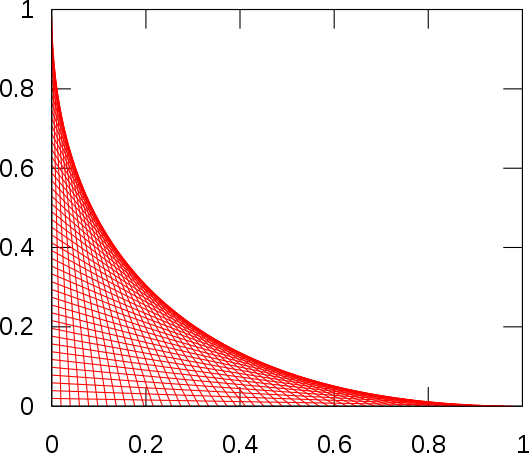
\includegraphics{envelope.png}
	\labfig{margin2}
\end{marginfigure}
Así tenemos dos nuevas coordenadas $[p,g(p)]$, relacionadas con $[x,f(x)]$ mediante
\vspace{-5pt}
\begin{equation} \label{4.1.1}
    \begin{matrix}
        p(x)=f'(x) && \color{blue}g(p)\color{black}=f(x(p))-x(p)\color{blue}p\color{black} &&[x,f(x)] \mapsto [p,g(p)] \\
        x(p)=(f')^{-1}(p) &&  \color{blue}f(x) \color{black}=p(x)\color{blue}x\color{black}+g(p(x))  && [p,g(p)] \mapsto [x,f(x)]\
    \end{matrix}
\end{equation} \refstepcounter{subsection}
Donde la primera expresión es la \textit{Transformada de Legendre}, y será invertible (la segunda expresión) siempre que $f'(x)$ sea invertible (cierto si $f''(x)\neq 0$).
\subsection{Varias variables}
Si ahora tenemos $f(\{x_i,y_i\})$ donde $\{y_i\}$ son las variables sobre las que queremos hacer la transformada, la transformada es entonces
\begin{equation} \label{4.1.2}
    \begin{matrix}
        p_i(\{x_i,y_i\})=\frac{\partial f}{\partial y_i} && g(\{x_i,\color{blue}p_i\color{black}\}) =f(\{x_i,y_i(\{x_i,p_i\})\}) -\sum_j \color{blue}p_j\color{black} y_j(\{x_i,p_i\})  &&[y_i,f] \mapsto [p_i,g] \\
        y_i(\{x_i,p_i\})=\left[\frac{\partial f}{\partial y_i}\right]^{-1} && f(\{x_i,\color{blue}y_i\color{black}\}) =\sum_j \color{blue}y_j\color{black} p_j (\{x_i,y_i\})  +g(\{x_i,p_i(\{x_i,y_i\})\}) &&[p_i,g] \mapsto [y_i,f]\\
    \end{matrix}
\end{equation} \refstepcounter{subsection}
La transformación será inversible si el jacobiano de $y_i \mapsto p_i$ es no nulo.
\subsubsection{Transformada de Legendre del Lagrangiano}
Ahora si tenemos $\pazocal{L}(\{q_j,\dot{q}_j\};t)$, $\{\dot{q}_j\}$ serán nuestras antiguas variables y las nuevas variables serán $\partial_{\dot{q}_j}\pazocal{L}=p_j$, los momentos generalizados o conjugados. Entonces aplicando (4.1.2) llegamos a (3.1.2)
\begin{equation} \label{4.1.3}
        p_i(\{q_i,\dot{q}_i\};t)=\frac{\partial \pazocal{L}}{\partial q_i} \ \ \ \ \ \  g(\{q_i,p_i\};t) =\pazocal{L}(\{q_i,p_i\};t) -\sum_j^s \dot{q}_j (\{q_i,p_i\}) p_j = -\pazocal{H}
\end{equation} \refstepcounter{subsection}
De esta forma, $\pazocal{H}$ es equivalente a la \textit{Transformada de Legendre} de $\pazocal{L}$ con respecto a los $\dot{q}_j$, y esta es inversible, la demostración de que el jacobiano $[\partial_{\dot{q}_j}p_i]$ es no nulo bajo ciertas circumstancias se deja como un ejercicio al lector.

De esta forma, no hemos perdido ninguna información del sistema al pasar de $\pazocal{L}$ a $\pazocal{H}$, y a continuación reformularemos las ecuaciones del movimiento en función de esta cantidad de una forma equivalente a la fomulación lagrangiana.
\section{Ecuaciones de Hamilton} \refstepcounter{subsection}
Si hacemos la diferencial exacta de $\pazocal{H}$ usando la regla de la cadena tenemos
\begin{equation} \label{4.2.1}
    d\pazocal{H} = \sum^s\left(\frac{\partial \pazocal{H}}{\partial q_j}dq_j+\frac{\partial \pazocal{H}}{\partial p_j}dp_j\right)+\frac{\partial \pazocal{H}}{\partial t} dt
\end{equation} \refstepcounter{subsection}
Si por otro lado hacemos el diferencial de $\pazocal{H}$ desde (3.1.2) o (4.1.3)
\begin{equation} \label{4.2.2}
    d\pazocal{H} = \sum^s\left(p_j d\dot{q}_j+\dot{q}_j dp_j\right)-d\pazocal{L}
\end{equation} \refstepcounter{subsection}
si $d\pazocal{L}$ es por regla de la cadena, y usando (2.2.1) y (2.2.2)
\begin{equation} \label{4.2.3}
    d\pazocal{L}= \sum^s\left(\frac{\partial \pazocal{L}}{\partial q_j}dq_j+\frac{\partial \pazocal{L}}{\partial \dot{q}_j}d\dot{q}_j\right) + \frac{\partial \pazocal{L}}{\partial t}dt = \sum^s\left(\dot{p}_j dq_j+p_j d\dot{q}_j\right) + \frac{\partial \pazocal{L}}{\partial t}dt
\end{equation} \refstepcounter{subsection}
Sustituyendo (4.2.3) en (4.2.2)
\begin{equation} \label{4.2.4}
    d\pazocal{H} = \sum^s p_j d\dot{q}_j+\dot{q}_j dp_j-\sum^s \dot{p}_j dq_j+p_j d\dot{q}_j - \frac{\partial \pazocal{L}}{\partial t}dt = \sum^s \dot{q}_j dp_j-\dot{p}_j dq_j - \frac{\partial \pazocal{L}}{\partial t}dt
\end{equation} \refstepcounter{subsection}
Como $dq_j$, $dp_j$ y $dt$ son funciones independientes y arbitrarias, podemos igualar término a término (4.2.4) y (4.2.1), de tal forma que obtenemos tres ecuaciones
\Large \begin{equation} \label{4.2.5}
    \boxed{\dot{q}_j = \frac{\partial \pazocal{H}}{\partial p_j} \ \ \ \ \ \ \dot{p}_j= -\frac{\partial \pazocal{H}}{\partial q_j}}
\end{equation} \refstepcounter{subsection} \normalsize
Estas dos primeras ecuaciones son las \textit{Ecuaciones de Hamilton} del movimiento o \textit{Ecuaciones canónicas}. Por otro lado tenemos la tercera ecuación, que junto a (3.1.2)
\begin{equation} \label{4.2.6}
    \frac{\partial \pazocal{H}}{\partial t} = - \frac{\partial \pazocal{L}}{\partial t} = \frac{d \pazocal{H}}{dt}
\end{equation} \refstepcounter{subsection}
De esta forma, si $\pazocal{H}$ no depende explícitamente del tiempo, este se conserva.

Para aplicar estas ecuaciones en un sistema holonómico tenemos que hayar primero $\pazocal{L}$, tras esto hallar los momentos generalizados y despues invertir la relación, tal que
\begin{equation} \label{4.2.7}
    p_j = \frac{\partial \pazocal{L}}{\partial \dot{q}_j}=p_j(\{q_k,\dot{q}_k\};t) \rightarrow \dot{q}_j = \dot{q}_j(\{q_k,p_k\};t)
\end{equation} \refstepcounter{subsection}
Entonces usamos la ecuación (4.1.3) con mucho cuidado de reemplazar todas las $\dot{q}_j$ por (4.2.7), y ya tendremos $\pazocal{H}$ en una forma que nos permita resolverlo usando (4.2.5).

Además, usando (4.1.3) podemos escribir $\pazocal{L}$ como
\begin{equation} \label{4.2.7}
    \pazocal{L}(\{q_i,p_i\};t) = \sum_j^s p_j \dot{q}_j (\{q_i,p_i\};t) -\pazocal{H}(\{q_i,p_i\};t)
\end{equation} \refstepcounter{subsection}
Si hacemos la acción de ese lagrangiano tendremos, y al extremizarla se puede comprobar que se obtienen (4.2.5)
\begin{equation} \label{4.2.7}
    S = \int_{t_A}^{t_B} \left(\sum_j^s p_j \dot{q}_j -\pazocal{H}\right) dt
\end{equation} \refstepcounter{subsection}
Para ello, aplicamos los metodos explicados en el Capítulo 1, teniendo en cuenta que $\pazocal{L}$ no depende de $\dot{p}_i$ 
\[
    \delta S = 0 = \int_{t_A}^{t_B} \delta \pazocal{L} dt = \int_{t_A}^{t_B} \sum_i\left(\frac{\partial \pazocal{L}}{\partial q_i} \delta q_i + \frac{\partial \pazocal{L}}{\partial \dot{q}_i} \delta \dot{q}_i + \frac{\partial \pazocal{L}}{\partial p_i} \delta p_i\right) dt
\]
Integrando el segundo término por partes como en (1.2.1), usando que $\delta \dot{q}_i =  \dot{(\delta q_i)}$
\[
    \delta S = 0 = \int_{t_A}^{t_B} \sum_{i}\left[\left(\frac{\partial \pazocal{L}}{\partial q_i} - \frac{d}{dt}\left(\frac{\partial \pazocal{L}}{\partial \dot{q}_i}\right)\right) \delta q_i + \frac{\partial \pazocal{L}}{\partial p_i}\delta p_i\right] dt
\]
Haciendo las derivadas de $\pazocal{L}$ obtenemos
\[
    \delta S = 0 = \int_{t_A}^{t_B} \sum_{i}\left[\left(-\frac{\partial \pazocal{H}}{\partial q_i} - \dot{p}_i\right) \delta q_i + \left(\dot{q}_i-\frac{\partial \pazocal{H}}{\partial p_i}\right)\delta p_i\right] dt
\]
Y ahora, establecemos que los términos entre paréntesis deben ser 0, puesto que las variaciones son arbitrarias e independientes, obteniendo (4.2.5).
\vspace{-20pt}
\subsubsection{Ejemplo}
Un ejemplo sencillo es el péndulo simple donde 
\[\pazocal{L}=\frac{1}{2}ml^2\dot{\theta}^2+mgl\cos{\theta} \ \ \ \ \ \ p_\theta = \frac{\partial \pazocal{L}}{\partial \dot{\theta}}=ml^2\dot{\theta} \ \ \ \ \ \ \dot{\theta}=\frac{p_\theta}{ml^2}=\dot{\theta}(p_\theta)\]
Sustituyendo tenemos 
\[\pazocal{H}=p_\theta \dot{\theta} -\pazocal{L}=\frac{p_\theta^2}{ml^2} - \frac{p_\theta^2}{2ml^2}-mgl\cos\theta = \frac{p_\theta^2}{2ml^2}-mgl\cos\theta = T+U\]

Ahora aplicamos (4.2.5.A), tal que $\dot{\theta} = p_\theta/ml^2$, de donde sacamos que $\dot{p}_\theta=ml^2 \ddot{\theta}$ y de (4.2.5.B) sacamos $\dot{p}_\theta=-mgl\sin\theta$, igualando y depejando tenemos $\ddot{\theta} + g/l \sin\theta = 0$, la ecuación del movimiento.
\subsubsection{Comparación Lagrange-Hamilton}
La formulación Lagrangiana es mejor para tratar con ligaduras, pero la hamiltoniana nos permite reducir el orden de la ecuación diferencial resultante cuando no hay dependencia explícita en una o varias de las $q_j$, puesto que en (3.1.5) $  \pazocal{L}$ sigue dependiendo de $\dot{q}_j$, solo conseguimos reducir en 1 el orden de un ecuación de E-L, mientras que en la formulación hamiltoniana, si una variable es cíclica, es decir $\partial_{q_j}\pazocal{H}=0$, entonces ya hemos resuelto $p_j=\alpha$ por (4.2.5.B) y también por definición $\pazocal{H}$ no depende de $q_j$, de esta forma nos hemos eliminado dos dependencias y reducir el orden en 2 unidades, podemos integrar $q_j$ usando (4.2.5.A) que como no depende de $q_j$ es una EDO separable. 
\section{Espacio de fase} \refstepcounter{subsection}
El hecho de que solo haya una sola solución para las ecuaciones del movimiento, es decir, que solo hay una posible trayectoria dadas unas condiciones dadas, significa que el sistema con el que estamos tratando es \textit{determinista}.

Si es el espacio de configuración es $\{q_j\}$ para un $t$ dado, entonces definimos el \textbg{Espacio de fase} como $\{q_j,p_j\}$, donde $\{p_j\}$ es el espacio de momentos o impulsos.

Este espacio es de dimensión $2s$ y nos da toda la información dinámica del sistema pues nos permite predecir su evolución, puesto que con unas condiciones iniciales de posición y momento (o velocidad) definidas por unas coordendas del espacio de fase, podemos usar (4.2.5) (Ecs. H.) para hallar la evolución del sistema.

\subsection{Diagrama de fases}
Es la trayectoria que sigue un sistema en el espacio de fase, normalmente representada en un conjunto de $s$ planos bidimensionales como una curva en cada uno de ellos, cuyos ejes representan $q_j$ y $p_j$, donde por cada punto en un $t$ dado solo puede pasar una sola trayectoria, de lo contrario el sistema no sería determinista, ya que de unas mismas condiciones iniciales podría evolucionar de varias formas.

Además si $\pazocal{H}$ se conserva, entonces por cada punto del espacio de fase solo puede pasar una trayectoria independientemente del tiempo.

\subsubsection{Ejemplo}
\begin{marginfigure}[0cm]
	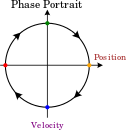
\includegraphics{phase.png}
	\labfig{margin3}
\end{marginfigure}
Como ejemplo vamos a ver un péndulo, tomando las expresiones del ejemplo de (4.2), donde las coordenadas del espacio de fases son $(\theta,p_\theta)$, si $\theta << 1$, tenemos $\ddot{\theta}+\frac{g}{l}\theta=0$, cuya solución, donde $\omega^2=g/l$, es
\[\theta = A \sin{(\omega t + \theta_0)}+ B \cos{(\omega t + \theta_0)} \ \ \ \ \dot{\theta} = A\omega \cos{(\omega t + \theta_0)}- B \omega \sin{(\omega t + \theta_0)} \ \ \ \ p_\theta = ml^2 \dot{\theta}\]
\[\theta^2 + \frac{p_\theta^2}{\omega^2 m^2l^4}=A^2+B^2 \mbox{ (elipse)}\]
\subsection{Teorema de Liouville} \refstepcounter{subsection}
\subsubsection{Volumen en el espacio de fase}
Definimos el volumen en el espacio de fases como
\begin{equation} \label{4.3.1}
    V = \prod_j^s \Delta q_j \Delta p_j
\end{equation} \refstepcounter{subsection}
Donde $\Delta q_j \Delta p_j$ es el área en uno de los $s$ planos.

Si ahora tenemos una serie de condiciones iniciales distribuidas dentro de una región volumétrica del espacio de fases, siendo $\pazocal{N}$ el número de condiciones iniales dentro de $V$, entonces si consideramos como la frontera de $V$ se transforma con el tiempo para dar $V'$, entonces $\pazocal{N}$ se conserva, puesto que para que una trayectoria entre o salga del volumen sería necesario que cortase una trayectoria de la frontera, lo cual no puede ocurrir en un sistema determinista.
\subsubsection{Teorema de Liouville} \refstepcounter{subsection}
El volumen $V(S)$ dentro de una superficie $S(t)$ del espacio de fase se conserva.
\begin{equation} \label{4.3.2}
    \frac{dV}{dt}=0 \implies \frac{d\rho}{dt} = 0 \ \ \ \ \rho = \frac{\pazocal{N}}{V}
\end{equation} \refstepcounter{susection}

\textbf{Demostración intuitiva}

Sean $\mathbf{z}=(\mathbf{q},\mathbf{p})$, $\mathbf{v}=\dot{\mathbf{z}}=(\dot{\mathbf{q}},\dot{\mathbf{p}})$, y $\mathbf{\nabla} = (\mathbf{\nabla}_\textbf{q},\mathbf{\nabla}_\textbf{p})$, entonces la divergencia de $\mathbf{v}$, tal que
\begin{equation} \label{4.3.4}
    \mathbf{\nabla} \cdot \mathbf{v} = \sum^s \frac{\partial \dot{q}_j}{\partial q_j} + \frac{\partial \dot{p}_j}{\partial p_j}
\end{equation} \refstepcounter{subsection}
entonces por el Teorema de la Divergencia
\begin{equation} \label{4.3.5}
    \int_V{\mathbf{\nabla} \cdot \mathbf{v} dV} = \int_S \mathbf{v} \cdot d\mathbf{S}
\end{equation} \refstepcounter{subsection}
La variación de $V$ en términos del tiempo es la siguiente, ya que $\mathbf{v}dt$ indica como se mueven las partículas de dentro de $V$, y multiplicando por $d\mathbf{S}$ nos indica como varía el volumen infinitesimalmente en un punto de la superficie, integrando en la superficie para ver la variación total de $V$ tenemos
\begin{equation} \label{4.3.6}
    dV=\int_S \mathbf{v} \cdot d\mathbf{S} dt \implies \frac{dV}{dt} = \int_S \mathbf{v} \cdot d\mathbf{S}
\end{equation} \refstepcounter{subsection}
Combinando (4.4.4), (4.4.5) y sustituyendo (4.4.3) llegamos a 
\begin{equation} \label{4.3.7}
    \frac{dV}{dt} = \int_V{\mathbf{\nabla} \cdot \mathbf{v} dV} = \int_V{\left(\sum^s \frac{\partial \dot{q}_j}{\partial q_j} + \frac{\partial \dot{p}_j}{\partial p_j}\right)dV}
\end{equation} \refstepcounter{subsection}
Ahora usando (4.2.5) (Ecs. H.) y que las parciales conmutan.
\begin{equation} \label{4.3.8}
    \frac{dV}{dt} = \int_V{\left(\sum^s \frac{\partial \pazocal{H}}{\partial q_j p_j} - \frac{\partial \pazocal{H}}{\partial p_j q_j}\right)dV} = 0
\end{equation} \refstepcounter{subsection}
\section{Paréntesis de Poisson} \refstepcounter{subsection}
Sea $f=f(\{q_j,p_j\};t)$ una función de las coordenadas canónicas, podemos hacer su derivada total con respecto al tiempo, tal que
\begin{equation} \label{4.4.1}
    \frac{d f}{dt} = \sum^s \left(\frac{\partial f}{\partial q_j}\dot{q}_j+\frac{\partial f}{\partial p_j}\dot{p}_j\right) + \frac{\partial f}{\partial t}
\end{equation} \refstepcounter{subsection}
Usando (3.2.5) (Ecs. H.) llegamos a 
\begin{equation} \label{4.4.2}
\frac{d f}{dt} = \sum^s \left(\frac{\partial f}{\partial q_j}\frac{\partial \pazocal{H}}{\partial p_j}-\frac{\partial f}{\partial p_j}\frac{\partial \pazocal{H}}{\partial q_j}\right) + \frac{\patial f}{\partial t} = [f,\pazocal{H}] + \frac{\partial f}{\partial t}
\end{equation} \refstepcounter{subsection}
Dónde $[f,\pazocal{H}]$ es el \textit{paréntesis de Poisson} de $f$ y $\pazocal{H}$, en general lo definimos para dos funciones como
\begin{equation} \label{4.4.3}
    [f,g]=  \sum^s \left(\frac{\partial f}{\partial q_j}\frac{\partial g}{\partial p_j}-\frac{\partial f}{\partial p_j}\frac{\partial g}{\partial q_j}\right)
\end{equation} \refstepcounter{subsection}
Sus propiedades algebraicas son muy similares a aquellas del producto vectorial puesto que su expresión es muy similar, son sencillas de verificar reemplando a fuerza bruta en (4.4.3).
\begin{itemize}
    \item Es alternada $[f,g]=-[g,f]$ y $[f,f]=0$.
    \item Si $[f,g]=0 \iff [f,g]=[g,f]=0$ las funciones conmutan.
    \item Es bilineal, $[f,\alpha g + \beta h] = \alpha [f,g] + \beta [f,h]$.
    \item Existe una regla del producto $[f,gh]=g[f,h]+h[f,g]$.
    \item Se verifica la \textit{Identidad de Jacobi}, $\left[f,[g,h]\right]+\left[h,[f,g]\right]+\left[g,[h,f]\right]=0$.
\end{itemize}
Otra regla del producto que se verifica, usando la conmutividad de las derivadas parciales, es $\frac{\partial}{\partial t}[f,g]=[\frac{\partial f}{\partial t},g]+[f,\frac{\partial g}{\partial t}]$.

Si la función $f$ no depende explícitamente del tiempo, entonces si $f$ conmuta con $\pazocal{H}$, eso implica por (4.4.2) y las propiedades anteriores, que $f$ se conserva.

Además, si tenemos dos cantidades conservadas $f$ y $g$, entonces tenemos que, usando la \textit{Identidad de Jacobi}, se conserva su paréntesis
\begin{equation} \label{4.4.5}
    \frac{d}{dt}[f,g]=0
\end{equation}

Si hacemos $[q_k,\pazocal{H}]$ y $[p_k,\pazocal{H}]$ aplicando (4.4.3) y (3.2.5) (Ecs. H.), obtenemos las ecuaciones del movimiento expresadas en términos de \textit{paréntesis de Poisson}.
\begin{equation} \label{4.4.6}
    \boxed{[q_k,\pazocal{H}] = \dot{q}_k \ \ \ \ \ [p_k,\pazocal{H}]=\dot{p}_k}
\end{equation}
Tenemos también los paréntesis de \textit{paréntesis de Poisson} fundamentales
\begin{equation} \label{4.4.7}
    [q_k,q_l]=[p_k,p_l]=0 \ \ \ \ \ [q_k,p_l]=\delta_{kl}
\end{equation}
En mecánica cuántica se define un operador similar, y expresar expresar sistemas en términos de \textit{paréntesis de Poisson} nos permite cuantizarlos. Un ejemplo es que (4.4.2) se convierte en la ecuación de \textit{Heissenberg}.

No hay mucho detalle en esta sección por que no es muy relevante para este curso, se incluye para familiarizarse con este formalismo.


\pagelayout{wide} % No margins
\addpart[Fuerzas centrales y sistemas no inerciales]{\fontsize{55pt}{0pt} \setstretch{2} \textbeuron{Fuerzas centrales sistemas no inerciales}}
\pagelayout{margin} % Restore margins

\chapter{Fuerzas centrales} 
\refstepcounter{subsection}
Llamamos fuerza central a toda fuerza $\mathbf{F}(\mathbf{r})=F(\mathbf{r}) \hat{\mathbf{e}}_r \label{5.0.1} \inlineeqnum$, es decir, que ocurre en dirección radial a un punto determinado, si además esta fuerza central es conservativa, es equivalente a $\mathbf{F}(r)=F(r) \hat{\mathbf{e}}_r \label{5.0.2} \inlineeqnum$, es decir que es esférica simétricamente y solo depende de la distancia al origen, ya que
\[\mathbf{F}=F(r) \hat{\mathbf{e}}_r=-\nabla U(r,\theta,\varphi)=\frac{\partial U}{\partial r}\hat{\mathbf{e}}_r + \frac{1}{r}\frac{\partial U}{\partial \theta}\hat{\mathbf{e}}_\theta+\frac{1}{r\sin\theta}\frac{\partial U}{\partial \varphi}\hat{\mathbf{e}}_\varphi \implies \frac{\partial U}{\partial \theta}=\frac{\partial U}{\partial \varphi}=0\]
puesto que $1/r$ y $1/r\sin\theta$ no pueden ser 0, esto implica que $U=U(r)$ y $F=F(r)$, además llegamos a la siguiente expresión de $F$
\begin{equation} \label{5.0.3}
    F(r)=-\frac{\partial U}{\partial r}
\end{equation} \refstepcounter{subsection}
La recíproca, que $\mathbf{F}(r)=F(r) \hat{\mathbf{e}}_r$ es conservativa se puede obtener calculando su rotacional y verificando que es igual a 0.
\section{Problema de los dos cuerpos} \refstepcounter{subsection}
\begin{marginfigure}[-2cm]
    \def\svgwidth{125 pt}
    \tiny
	\input{images/centralf.pdf_tex}
	\labfig{margin2}
\end{marginfigure}
Si tenemos dos masas $m_1$ y $m_2$ con posiciones $\mathbf{r}_1$ y $\mathbf{r}_2$, de tal forma que sufren cada una una fuerza central conservativa creada por la otra masa, siguiendo la tercera ley de newton, entonces $U=U(r)$, donde $r=|\mathbf{r}_1-\mathbf{r}_2|=|\mathbf{r}| \label{5.1.1} \inlineeqnum$, tal que $\mathbf{r}=\mathbf{r}_1-\mathbf{r}_2 \label{5.1.2} \inlineeqnum$.

Podemos definir también el centro de masas del sistema de ambas masas, que se encuentra necesariamente en un punto intermedio entre ambas masas, y más cercano a la masa mayor
\begin{equation} \label{5.1.3}
    \mathbf{R} = \frac{1}{M}\sum^n{m_i \mathbf{r_i}} = \frac{m_1 \mathbf{r}_1 + m_2 \mathbf{r}_2}{m_1+m_2} \ \ \ \ \ M=\sum^n m_i
\end{equation} \refstepcounter{subsection}
De esta forma podemos hacer el cambio de las coordenadas $(\mathbf{r}_1,\mathbf{r}_2) \mapsto (\mathbf{r},\mathbf{R})$, que podemos invertir despejando $\mathbf{r}_1$ y de (5.1.2) y (5.1.3) e igualando para despejar $\mathbf{r}_2$, después sacamos $\mathbf{r}_1$ de una de las anteriores, tal que
\begin{equation} \label{5.1.4}
    \mathbf{r}_1 = \mathbf{R} + \frac{m_2}{M}\mathbf{r} \ \ \ \ \ \ \mathbf{r}_2 = \mathbf{R} - \frac{m_1}{M}\mathbf{r}
\end{equation} \refstepcounter{subsection}
Ahora podemos escribir $\pazocal{L}$ del sistema, para la energía cinética, veremos que los términos cruzados se cancelan
\begin{equation} \label{5.1.5}
    T=\frac{1}{2}m_1(\dot{\mathbf{r}}_1)^2+\frac{1}{2}m_2(\dot{\mathbf{r}}_2)^2=\frac{1}{2}M(\dot{\mathbf{R}})^2 + \frac{1}{2}\mu(\dot{\mathbf{r}})^2 \ \ \ \ \ 
    \boxed{\mu = \frac{m_1 m_2}{m_1+m_2}} \ \ \ \ \ \ \ U = U(r)
\end{equation} \refstepcounter{subsection}
\begin{equation} \label{5.1.6}
    \pazocal{L} = \pazocal{L}_{CM} + \pazocal{L}_{\mbox{\small rel}}= \left(\frac{1}{2}M(\dot{\mathbf{R}})^2\right) + \left(\frac{1}{2}\mu(\dot{\mathbf{r}})^2-U(r)\right)
\end{equation} \refstepcounter{subsection}
Es de notar que cuando la diferencia en las masas es muy grande, la masa reducida, $\mu$ tiende a la masa más pequeña.

De la ecuación (5.1.6) podemos concluir usando (E-L) que el momento asociado a $\mathbf{R}$ se conserva, puesto que que $\pazocal{L}$ no depende explícitamente de $\mathbf{R}$, entonces podemos llegar a tres ecuaciones resumidas en $M\ddot{\mathbf{R}}=0 \label{5.1.7} \inlineeqnum$, que indican que la velocidad del CM es constante.

Para el movimiento relativo en $\mathbf{r}$, aplicando (E-L), podemos llegar a tres ecuaciones que resuminos en $\mu\ddot{\mathbf{r}}=-\nabla U \label{5.1.8} \inlineeqnum$.

Entonces por (5.1.7), el sistema de referencia relativo al CM es un sistema inercial, de tal forma que estableciendo $\mathbf{R}=0$, podemos obtener las expresiones de $\mathbf{r}_1$ y $\mathbf{r}_2$ en el sistema del CM.
\begin{equation} \label{5.1.9}
    \mathbf{r}_1=\frac{m_2}{M}\mathbf{r} \ \ \ \ \ \mathbf{r}_2=-\frac{m_1}{M}\mathbf{r}
\end{equation} \refstepcounter{subsection}
Observando el dibujo de la página anterior, esta claro que en el sistema del CM, las posiciones de ambas masas deben estar en el mismo eje, es decir, sus vectores de posición son paralelos, puesto que $\mathbf{R}$ se encuentra siempre entre la recta que une a ambas masas.

Hay que tener cuidado por que $\mathbf{r}$ no es un vector posición, sino como definimos en (5.1.2), es la diferencia entre los dos vectores de posición.
\section{Conservación del momento angular}  \refstepcounter{subsection}
Definimos el momento angular total con respecto a O como $\mathbf{J} = \mathbf{J}_1 + \mathbf{J}_2 \label{5.1.10} \inlineeqnum$, donde $\mathbf{J}_i = \mathbf{r}_i \times \mathbf{p}_i = m_i \mathbf{r}_i \times \dot{\mathbf{r}}_i \label{5.1.11} \inlineeqnum$. La derivada del momento angular será entonces
\begin{equation} \label{5.1.12}
    \dot{\mathbf{J}_i}= m \left(\dot{\mathbf{r}}_i \times \dot{\mathbf{r}}_i + \mathbf{r}_i \times \ddot{\mathbf{r}}_i \right) = m \mathbf{r}_i \times \mathbf{r}_i = \mathbf{r}_i \times \mathbf{F}_i
\end{equation} \refstepcounter{subsection}
Entonces, usando la 3ª LN, (5.1.2) y (5.0.1), el momento angular total se conserva.
\begin{equation} \label{5.1.13}
    \dot{\mathbf{J}}=\mathbf{r}_1 \times \mathbf{F}_{12}+\mathbf{r}_2 \times \mathbf{F}_{21}=(\mathbf{r}_1-\mathbf{r}_2)\times \mathbf{F}=F \mathbf{r} \times \hat{\mathbf{u}}_r = 0
\end{equation} \refstepcounter{subsection}
El momento angular total en el sistema del CM es entonces, usando (5.1.9)
\begin{equation} \label{5.1.14}
    \mathbf{J} = \frac{m_1 m_2^2}{M^2} (\mathbf{r}\times \dot{\mathbf{r}})+ \frac{m_2 m_1^2}{M^2} (\mathbf{r}\times \dot{\mathbf{r}}) = \mu (\mathbf{r}\times \dot{\mathbf{r}})
\end{equation} \refstepcounter{subsection}
Como este se conserva puesto que sigue siendo inercial, esto implica que el movimiento de ambas masas debe ocurrir en un plano*, el perpendicular a $\mathbf{J}$.

Entonces podemos expresar la configuración del sistema con coordenadas polares, puesto que tenemos dos grados de libertad. Expresando el lagrangiano del sistema en coordenadas polares usando (5.1.6) y $\dot{\mathbf{r}}=d{(r \hat{\mathbf{u}}_r)}/dt=\dot{r}\hat{\mathbf{u}}_r + r \dot{\varphi}\hat{\mathbf{u}}_\varphi$ tenemos
\begin{equation} \label{5.1.15}
    \pazocal{L} = \frac{1}{2}\mu(\dot{\mathbf{r}})^2-U(r) = \frac{1}{2}\mu\left(\dot{r}^2+r^2\dot{\varphi}^2\right)-U(r)
\end{equation} \refstepcounter{subsection}
Vemos que entonces $\varphi$ es ignorable pues no aparece explícitamente y entonces su momento se conserva
\begin{equation} \label{5.1.16}
    p_\varphi = J = \frac{\partial \pazocal{L}}{\partial \dot{\varphi}} = \mu r^2 \dot{\varphi} \ \ \ \  \dot{p_\varphi} = 0
\end{equation} \refstepcounter{subsection}
Lo cual es exáctamente el módulo de $\mathbf{J}=\mu (r\hat{\mathbf{u}_r}\times (\dot{r}\hat{\mathbf{u}_r} + r \dot{\varphi} \hat{\mathbf{u}_\varphi}))= \mu r^2 \dot{\varphi}\hat{\mathbf{u}_z}$
\vspace{5pt}
\subsection{Esféricas *}
Podemos también demostrar que el movimiento ocurre en un plano escribiento el lagrangiano usando coordenadas esféricas, similar a (5.2.6), donde $\dot{\mathbf{r}}=d{(r \hat{\mathbf{u}}_r)}/dt=\dot{r}\hat{\mathbf{u}}_r + r \dot{\theta }\hat{\mathbf{u}}_\theta + r\sin \theta \dot{\varphi} \hat{\mathbf{u}}_\varphi$, tal que 
\begin{equation} \label{5.1.17}
    \pazocal{L} = \frac{1}{2}\mu(\dot{\mathbf{r}})^2-U(r) = \frac{1}{2}\mu\left(\dot{r}^2+r^2\dot{\theta}^2 + r^2 \sin^2 \theta \dot{\varphi}^2\right)-U(r)
\end{equation} \refstepcounter{subsection}
De esta forma vemos que $\varphi$ es la ignorable, de tal forma que su momento asociado se conservará
\begin{equation} \label{5.1.18}
    p_\varphi = \frac{\partial \pazocal{L}}{\partial \dot{\varphi}} = \mu r^2 \sin^2 \theta \dot{\varphi} \ \ \ \  \dot{p_\varphi} = 0
\end{equation} \refstepcounter{subsection}
Si ahora consideramos $\mathbf{J}$ en estas coordenadas usando (5.2.5)
\begin{equation} \label{5.1.19}
    \mathbf{J} = \mu (\mathbf{r} \times (\dot{r}\hat{\mathbf{u}}_r + r \dot{\theta}\hat{\mathbf{u}}_\theta + r\sin \theta \dot{\varphi} \hat{\mathbf{u}}_\varphi))=-\mu r^2 \sin \theta \dot{\varphi} \hat{\mathbf{u}}_\theta + \mu r^2 \dot{\theta}\hat{\mathbf{u}}_\varphi
\end{equation} \refstepcounter{subsection}
Como $\mathbf{J}$ se conserva, sus componentes se conservan, y entonces usando (5.2.10) en (5.2.9), verificamos que el movimiento ocurre en un plano, donde $\theta$ es constante.
\begin{equation} \label{5.1.20}
    p_\varphi = \mu r^2 \sin^2 \theta \dot{\varphi} = J_\theta \sin\theta \implies \frac{d}{dt} \sin\theta = \dot{\theta} \cos \theta = 0 \implies \dot{\theta} = 0
\end{equation} \refstepcounter{subsection}
\vspace{-30pt}
\subsubsection{Velocidad areolar}
Si consideramos el área que barre $\mathbf{r}$ en un pequeño incremento del tiempo como si fuera un triángulo, tenemos que, donde el primer término es la base del triángulo y el segundo la altura del triángulo, vemos que esta cantidad se conserva.
\begin{equation} \label{5.1.21}
    dA = \frac{1}{2} r\cdot r\dot{\varphi} dt \ \ \ \ \ \dot{A} = \frac{J}{2\mu} \ \ \ \ \ddot{A} = 0
\end{equation} \refstepcounter{subsection}
Esta ecuación se conoce como la segunda ley de \textit{Kepler}.
\section{Energía} \refstepcounter{subsection}
La energía (conservada e igual a $\pazocal{H}$), es, por (5.2.6) y (5.2.7)
\begin{equation} \label{5.1.22}
    E = T+U = \frac{1}{2}\mu\left(\dot{r}^2+r^2\dot{\varphi}^2\right)+U(r)=\frac{1}{2}\mu\dot{r}^2 + \frac{J^2}{2\mu r^2}+U(r)
\end{equation} \refstepcounter{subsection}
La ecuación (5.3.1) es una EDO de primer orden separable que nos permite hallar $r(t)$, invirtiendo la siguiente expresión
\begin{equation} \label{5.1.23}
    \int_{r_0}^r{\left[\frac{2}{\mu}\left(E-U(r)\right)-\frac{J^2}{\mu^2 r^2}\right]^{-\frac{1}{2}}dr}=t-t_0
\end{equation} \refstepcounter{subsection}

Usando (5.2.7) podemos encontrar $\varphi(t)$ una vez tenemos $r(t)$, de forma similar al formalismo Hamiltoniano.
\section{Ecuación del movimiento} \refstepcounter{subsection}
Haciendo (2.2.1)(E-L) con respecto a $r$ obtenemos la ecuación del movimiento del sistema
\begin{equation} \label{5.1.24}
    \mu \ddot{r} = \mu r \dot{\varphi}^2 - \frac{\partial U}{\partial r} = \frac{J^2}{\mu r^3}+ F(r)
\end{equation} \refstepcounter{subsection}

Nos va a interesar encontrar $r(\varphi)$ para no tener una expresión paramétrica de ambos sino la ecuación de una curva, para ello haremos el cambio de variable $u=1/r$.

Usando la regla de la cadena, el teorema de la función inversa y (5.1.16)
\begin{equation} \label{5.1.25}
    \frac{d u}{d\varphi}  = -\frac{1}{r^2} \frac{dr}{d\varphi} = -\frac{1}{r^2} \frac{dr}{dt} \frac{dt}{d\varphi}= -\frac{1}{r^2} \dot{r} \frac{1}{\frac{d\varphi}{dt}}=-\frac{1}{r^2} \dot{r} \frac{1}{\dot{\varphi}}= -\frac{1}{r^2} \dot{r} \frac{r^2 \mu}{J} = -\frac{\mu \dot{r}}{J}
\end{equation} \refstepcounter{subsection}
\begin{equation} \label{5.1.26}
    \frac{d^2 u}{d\varphi^2}  = \frac{d}{d\varphi}\left(-\frac{\mu \dot{r}}{J}\right)=-\frac{\mu}{J} \frac{d \dot{r}}{dt} \frac{dt}{d\varphi} = -\frac{\mu}{J} \frac{d \dot{r}}{dt} \frac{1}{\frac{d\varphi}{dt}} = -\frac{\mu}{J} \ddot{r} \frac{1}{\dot{\varphi}}= - \frac{\mu^2}{J^2} r^2 \ddot{r}
\end{equation} \refstepcounter{subsection}
Despejando $\ddot{r}$ de (5.4.3) y sustituyendo en (5.4.1) llegamos a la ecuación de la trayectoria, cuya solución es $r(\varphi)$
\begin{equation} \label{5.1.27}
    \frac{\partial^2 u}{\partial \varphi^2} + u = -\frac{\mu}{J^2 u^2}F(u) \iff \frac{\partial^2}{\partial \varphi^2}\left(\frac{1}{r}\right) + \frac{1}{r} = -\frac{\mu}{J^2}r^2F(r)
\end{equation} \refstepcounter{subsection}
\section{Potencial efectivo} \refstepcounter{subsection}
El primer término de la ecuación (5.4.1) se denomina fuerza centrífuga, a la que podemos asociar un potencial, tal que 
\begin{equation} \label{5.1.28}
    F_{\mbox{\small cf}} = \frac{J}{\mu r^3} = -\frac{\partial U_{\mbox{\small cf}}}{\partial r} \implies U_{\mbox{\small cf}} = \frac{J^2}{2\mu r^2}
\end{equation} \refstepcounter{subsection}
De esta forma las expresiónes (5.4.1) y (5.3.1) nos quedan
\begin{equation} \label{5.1.29}
    \mu \ddot{r} = -\frac{\partial}{\partial r} (U_{\mbox{\small cf}}+U) = -\frac{\partial U_{\mbox{\small ef}}}{\partial r} \ \ \ \ \ \  U_{\mbox{\small ef}} = U(r) + \frac{J^2}{2\mu r^2}
\end{equation} \refstepcounter{subsection}
\begin{equation} \label{5.1.29}
    E = \frac{1}{2}\mu \dot{r}^2 + \left(\frac{J^2}{2\mu r^2}+U(r)\right) = \frac{1}{2}\mu\dot{r}^2 + U_{\mbox{\small ef}}(r)
\end{equation} \refstepcounter{subsection}
El primer término de (5.5.3) lo llamamos el término cinético y siempre es positivo, esto implica necesariamente la siguiente relación que determinará que valores de $r$ podrá tomar el sistema.
\begin{equation} \label{5.1.30}
    E\geq U_{\mbox{\small uf}}(r) \ \ \forall ts \ \ \ \ \ \ E = U_{\mbox{\small uf}}(r) \implies \dot{r}=0
\end{equation} \refstepcounter{subsection}


\clearpage
\section{Potenciales $-\gamma/r$}\refstepcounter{subsection}
Si tenemos un potencial de la forma siguiente, entonces el potencial efectivo asociado toma la siguiente expresión representada en la figura.
\begin{equation} \label{5.6.1}
    U(r) = -\frac{\gamma}{r} \ \ \ \ \gamma>0 \ \ \ \ \ \ U_{\mbox{\small ef}} =  \frac{J^2}{2\mu r^2} -\frac{\gamma}{r}
\end{equation} \refstepcounter{subsection}
\begin{figure}[h]
    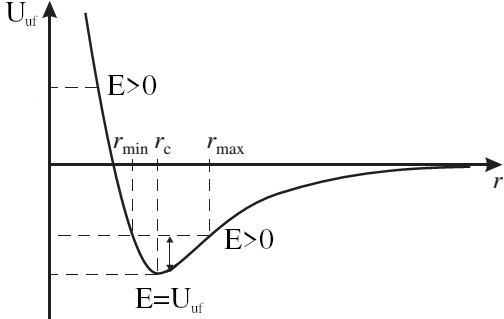
\includegraphics[width=12cm]{uf.png}
\end{figure}
Aplicando (5.5.4) podemos deducir ciertas propiedades del movimiento.

Si $E>0$, tenemos que la recta corta en un solo punto a $U_{\mbox{\small ef}}$, en ese punto serán iguales y la velocidad radial se anula. Esto nos indica que si r va disminuyendo, su velocidad radial es negativa pero su modulo va aumentando hasta que llega a $r_c$, donde la diferencia entre $E$ y $U_{\mbox{ \small ef}}$ es mayor y alcaza su pico, entonces el modulo de la velocidad radial disminuye hasta que se anula en el punto $r$ donde se cortan, entonces r volverá a aumentar, siendo su velocidad positiva y creciente, hasta alcanzar su pico en $r_c$, tras lo cual la velocidad decrece hasta un valor límite cuanto r tiende a infinito.

En cambio, si $E>0$, esta corta en dos puntos a $U_{ \mbox{\small ef}}$, donde la velocidad radial se anulará, lo que significa que $r$ esta acotado entre esos dos puntos $r_{\mbox{\small min}}$ y $r_{\mbox{\small max}}$, llamados \textit{periápside} y \textit{apoápside} respectivamente, entorno a los cuales oscilará, puesto que fuera de esa región no se cumple (5.5.4).

Estos valores pueden encontrarse igualando (5.6.1) a $E$ y resolviendo para $1/r$ como una ecuación cuadrática, obteniendo
\begin{equation} \label{5.6.2}
    \frac{1}{r}=\frac{\gamma \mu}{J^2}\left(1\pm\sqrt{1+\frac{2J^2 E}{\gamma^2 \mu}}\right)
\end{equation} \refstepcounter{subsection}

Diremos que una de trayectoria es cerrada cuando exista un periodo $\tau$ tal que $r(t+\tau)=r(t)$ y $\varphi(t+\tau)=\varphi(t) +2 \pi k$ para algún $k \in \mathbb{Z}$.

Si $E=U_{\mbox{\small ef}}$, la velocidad radial se anula y $r$ es constante, describiendo una órbita circular de radio $r_c$.

\section{Órbitas de Kepler} \refstepcounter{subsection}
Tenemos de nuevo $U(r)=-\gamma/r$ y $F(r)=-\gamma/r^2$ tal que $\gamma > 0$. Usando la ecuación de la trayectoria (5.4.4), tenemos que $F(u)=-\gamma u^2$, si $u=u(\varphi)$, entonces
\begin{equation} \label{5.7.1}
    u'' + \left(u -\frac{\mu \gamma}{J^2}\right) = 0 = u'' + \omega(\varphi) \rightarrow \omega'' = u'' \implies \omega'' + \omega = 0 
\end{equation} \refstepcounter{subsection}
Haciendo ese cambio de variable hemos encontrado una EDO facil de resolver, tal que , pudiendo escoger $\delta =0$ al escoger los ejes adecuados (el origen de $\varphi$)
\begin{equation} \label{5.7.2}
    \omega = A \cos{\varphi +\delta} \implies u(\varphi) = \omega + \frac{\mu \gamma}{J^2} = A \cos{\varphi} +\frac{\mu \gamma}{J^2} = \frac{\mu \gamma}{J^2}\left(1+ \frac{A J^2}{\mu \gamma} \cos(\varphi)\right)
\end{equation} \refstepcounter{subsection}
Renombrando ciertas constantes, usando que $A\geq0$y sustituyendo $u$ llegamos a 
\begin{equation} \label{5.7.3}
    \frac{1}{c} = \frac{\mu \gamma}{J^2}>0 \ \ \ \ \epsilon=\frac{A J^2}{\mu \gamma}\geq 0 \ \ \ \ \ \ r(\varphi) = \frac{c}{1+\epsilon \cos\varphi}
\end{equation} \refstepcounter{subsection}
Veremos que (5.7.3) es la ecuación de las secciones cónicas en coordenadas polares.
\subsection{Caso $0 \leq \epsilon < 1 $}
Si $0 \leq \epsilon < 1 $, entonces el denominador de (5.7.3) nunca se anula, lo que significa que $r$ va a estar acotado con extremos $r_{\mbox{\small min}}$ y $r_{\mbox{\small max}}$ que ocurrirán en $\cos \varphi = \{-1,1\}$
\begin{equation} \label{5.7.4}
    r_{\mbox{\small min}}= \frac{c}{1+\epsilon} \ \ \ \ \ \ r_{\mbox{\small max}} = \frac{c}{1-\epsilon}
\end{equation} \refstepcounter{subsection}
Como el denominador no se anula, $r(\varphi+2\pi k)=r(\varphi)$ para cualquier $k\in \mathbb{Z}$, es decir es periódica en $\varphi$, lo cual también implica que es cerrdada.

Si ahora expresamos (5.7.3) en cartesianas, primero definiendo las transformaciones
\begin{equation} \label{5.1.5}
    x = r\cos\theta \ \ \ \ y = r\sin \theta \ \ \ \ r^2=x^2+y^2
\end{equation} \refstepcounter{subsection}
\vspace{-15pt}
\begin{equation} \label{5.1.6}
    c = r +\epsilon r \cos\varphi = r+\epsilon x \rightarrow r = c-\epsilon x
\end{equation} \refstepcounter{subsection}
\vspace{-20pt}
\begin{equation} \label{5.1.7}
    (c-\epsilon x)^2 = c^2 + \epsilon^2 x^2 -2\epsilon c x = x^2 + y^2 \rightarrow x^2 +2 \frac{c\epsilon}{1-\epsilon^2}x +\frac{y^2}{1-\epsilon^2}=\frac{c^2}{1-\epsilon^2}
\end{equation} \refstepcounter{subsection}
Despejando c de (5.7.3) en (5.7.6), sustituyendo en (5.7.5) y operando llegamos a (5.7.7). Si ahora definimos las siguientes constantes
\begin{equation} \label{5.1.8}
    d = \frac{c\epsilon}{1-\epsilon^2} \ \ \ \ \ b^2 = \frac{c^2}{1-\epsilon^2} \ \ \ \ \ b^2 + d^2 = \frac{c^2}{(1-\epsilon^2)^2} = a^2
\end{equation} \refstepcounter{subsection}
\vspace{-15pt}
\begin{equation} \label{5.1.8}
    b^2 = a^2(1-\epsilon^2) \ \ (b<a) \ \ \ \ \ d=a\epsilon
\end{equation} \refstepcounter{subsection}
Podemos reescribir (5.7.7) y completar el cuadrado de $x$
\begin{equation} \label{5.1.7}
    x^2 +2dx +\frac{y^2}{1-\epsilon^2}=b^2 \rightarrow (x+d)^2 +\frac{y^2}{1-\epsilon^2}=b^2 + d^2 = a^2
\end{equation} \refstepcounter{subsection}
De esta forma pasando $a^2$ dividiendo y usando (5.7.9) obtenemos la ecuación de una elipse
\begin{equation} \label{5.1.7}
    \left(\frac{x+d}{a}\right)^2 +\left(\frac{y}{b}\right)^2=1
\end{equation} \refstepcounter{subsection}
\begin{figure}[H]
    \def\svgwidth{15 cm}
    \normalsize
	\input{images/orbit.pdf_tex}
	\labfig{margin2}
\end{figure}
\vspace{-40pt}
Como se puede apreciar en (5.7.11), el centro de la elipse esta desplazdo $d$ unidades hacía la derecha de $O$, la posición $m_2$.
\subsection{Caso $ç\epsilon = 1 $}
\subsection{Caso $ç\epsilon > 1 $}

% \chapter{Sistemas de referencia no inerciales} 
\refstepcounter{subsection}
Llamemos $\pazocal{S}_0$, al sistema de referencia inercial, que lleva asociado un origen espacial $\pazocal{O}_0 = \mathbf{O}_{\pazocal{S}_0}$, un origen temporal $\pazocal{O}_{t_0}=0_{\pazocal{S}_0}$, cuyos ejes cartesianos se encuentran fijos, con coordenadas $(x_0,y_0,z_0)$. Lo representamos por $\pazocal{S}_0 = \left\{\pazocal{O}_0,\pazocal{O}_{t_0},(\mathbf{e}_{x_0},\mathbf{e}_{y_0},\mathbf{e}_{z_0})\right\}$.

Tenemos otro sistema de referencia $\pazocal{S}$ no inercial, con sus orígenes, $\pazocal{O}$ y $\pazocal{O}_{t}$ que pueden ser iguales o distintos a los de $\pazocal{S}_0$, con sus ejes cartesianos fijos en él mismo, con coordenadas $(x,y,z)$, tal que $\pazocal{S} = \left\{\pazocal{O},\pazocal{O}_{t},(\mathbf{e}_x,\mathbf{e}_y,\mathbf{e}_z)\right\}$.

Definimos formalmente que los ejes estan fijos con respecto a un sistema de referencia cuando 
\begin{equation} \label{6.1.1}
    \left(\frac{d}{dt}\mathbf{e}_{j_0}\right)_{\pazocal{S}_0} = 0 \ \ \ \ \ \left(\frac{d}{dt}\mathbf{e}_j\right)_{\pazocal{S}} = 0 \ \ \ \ \ \forall j
\end{equation} \refstepcounter{subsection}
Entonces un sistema de referencia es no inercial cuando, para algún $j$,
\begin{equation} \label{6.1.1}
    \left(\frac{d}{dt}\mathbf{e}_j\right)_{\pazocal{S}_0} \neq 0 \iff \left(\frac{d}{dt}\mathbf{e}_{j_0}\right)_{\pazocal{S}} \neq 0 
\end{equation} \refstepcounter{subsection}
es decir, alguno de los vectores de $\pazocal{S}$ no es constante respecto a $\pazocal{S}_0$. También es un sistema no inercial en general cuando $\pazocal{O}$ este acelerado con respecto a un $\pazocal{S}_0$.
\section{Aceleración rectilínea}
\refstepcounter{subsection}
Si tenemos que $\pazocal{S}$ esta se mueve de forma rectilínea respecto a $\pazocal{S}_0$ con aceleración $\mathbf{A}=\dot{\mathbf{V}}$, donde $\mathbf{V}$ es la velocidad de $\pazocal{S}$ respecto a $\pazocal{S}_0$.

Si $\mathbf{r}_0$ y $\mathbf{r}$ son vectores de posición equivalentes en cada sistema de referencia, estos se relacionan por
\begin{equation} \label{6.1.1}
    \dot{\mathbf{r}}_0=\dot{\mathbf{r}}+\mathbf{V} \rightarrow \ddot{\mathbf{r}}_0=\ddot{\mathbf{r}}+\mathbf{A}
\end{equation} \refstepcounter{subsection}
Si ahora tenemos la 2LN, llegamos a que aparece lo que llamamos '\textit{fuerza inercial}' en el sistema no inercial
\begin{equation} \label{6.1.1}
    \mathbf{F} = m\ddot{\mathbf{r}}_0 = m\ddot{\mathbf{r}} + m \mathbf{A} \implies m\ddot{\mathbf{r}} = \mathbf{F}-m \mathbf{A} = \mathbf{F}+\mathbf{F}_{\mbox{\small iner.}}
\end{equation} \refstepcounter{subsection}
\vspace{-25pt}
\subsection{Mareas}
Vamos a asumir que ha habido un diluvio universal y la Tierra esta cubierta de océano. Las mareas son un fenómeno en el que la altura del mar varía con periodo de unas 12 horas.

Si tenemos un objeto $m$ en la superficie del océano. Considerando que la rotación de la Luna sobre la Tierra tiene un periodo mucho mayor que las mareas, podremos considerar el sistema de referencia de la Tierra como un sistema no inercial con aceleración rectilínea y que la Tierra y la Luna no rotan en ese intervalo temporal.
\begin{figure}[H]
    \def\svgwidth{15 cm}
    \normalsize
	\input{images/marea.pdf_tex}
	\labfig{margin2}
    \vspace{-75pt}
    \caption{Diagrama del sistema}
\end{figure}
\vspace{15pt}
La aceleración de la Tierra con respecto al CM de ambos cuerpos es la fuerza gravitatoria que sufre la tierra debida a la masa de la luna partido por la masa de la tierra, dirección a la Luna.
\begin{equation} \label{6.1.1}
    \mathbf{A} = -\frac{G M_L}{d_0^2} \mathbf{e}_{d_0}
\end{equation} \refstepcounter{subsection}

Entonces por (6.1.2) la fuerza inercial que sufre $m$ en su sistema de referencia es
\begin{equation} \label{6.1.1}
    \mathbf{F}_{\mbox{\small iner.}} = \frac{GmM_L}{d_0^2}\mathbf{e}_{d_0}
\end{equation} \refstepcounter{subsection} 
Además, $m$ sufre las fuerzas gravitatorias de la Tierra, la Luna, y la fuerza de Arquímedes del agua, tal que
\begin{equation} \label{6.1.1}
    \mathbf{F}_T = m\mathbf{g} \ \ \ \ \ \mathbf{F}_L = -\frac{GmM_L}{d^2}\mathbf{e}_d
\end{equation} \refstepcounter{subsection}
También deberíamos tener en cuenta la fuerza centrífuga de la rotación de la Tierra sobre su propio eje, pero la vamos a despreciar por que no es muy grande en comparación al resto.
Entonces, usando (6.1.2), la 2LN para $m$ nos queda
\begin{equation} \label{6.1.1}
    m \ddot{\mathbf{r}} = m\mathbf{g} + \mathbf{F}_A - GmM_L\left(\frac{\mathbf{e}_d}{d^2}-\frac{\mathbf{e}_{d_0}}{d_0^2}\right) = m\mathbf{g} + \mathbf{F}_A + \mathbf{F}_{\mbox{\small marea}}
\end{equation} \refstepcounter{subsection}
Los casos en los que $m$ se encuentra en los puntos $A$ y $B$, donde $\mathbf{e}_d=\mathbf{e}_{d_0}$, en el primer caso $d<d_0$ y en el segundo $d>d_0$, así podemos obtener el sentido de la fuerza de marea en esos puntos usando (6.1.6), como se observa en el diagrama 
\begin{equation} \label{6.1.1}
    \mathbf{F}_{\mbox{\small marea}}=-GmM_L\left(\frac{1}{d^2}-\frac{1}{d_0^2}\right)\mathbf{e}_d \ \ \ \ \ \begin{matrix}
        \mathbf{F}^A_{\mbox{\small marea}} \propto -\mathbf{e}_d \\
        \mathbf{F}^B_{\mbox{\small marea}} \propto \ \ \ \mathbf{e}_d
    \end{matrix}
\end{equation} \refstepcounter{subsection}
Cuando $m$ se encuentra en $C$ o $D$, $d^2=r^2+d_0^2$, y podemos hacer la siguiente aproximación por series de Taylor cuando $r<<d_0$, lo cual es cierto en este caso.
\begin{equation} \label{6.1.1}
    d = d_0\left[1+\left(\frac{r}{d_0}\right)^2\right]^{1/2} = d_0+ O\left(\left(\frac{r}{d_0}\right)^2\right)
\end{equation} \refstepcounter{subsection}
Por otro lado $d\mathbf{e}_d = d_0\mathbf{e}_{d_0}+ \mathbf{r}$, usando (6.1.7) llegamos a que
\begin{equation} \label{6.1.1}
    \mathbf{e}_d \approx \mathbf{e}_{d_0}+ \frac{\mathbf{r}}{d_0}
\end{equation} \refstepcounter{subsection}
Entonces usando (6.1.6), (6.1.8) y (6.1.9) llegamos a que, como se observa en el diagrama
\begin{equation} \label{6.1.1}
    \mathbf{F}_{\mbox{\small marea}}\approx-GmM_L\frac{\mathbf{r}}{d_0^3} \propto -\mathbf{r}
\end{equation} \refstepcounter{subsection}
Entonces de (6.1.7) y (6.1.10) concluimos que horizontalmente las fuerzas son hacía fuera, y verticalmente son hacía dentro, por lo que de forma cualitativa nos podemos imaginar de forma cualitativa que el océano hace la curva achatada dibujada en el diagrama.

El hecho de que la Tierra este en rotación sobre su propio eje explica el periodo de 12 horas de las mareas, puesto que al transcurrir medio día, te encuentras en el punto antipodal al que te encontrabas, pero la altura de la marea es muy similar.

\subsubsection{Diferencia de altura}
Ahora queremos determinar la diferencia de altura del océano entre $A$ y $C$.

Como $\mathbf{F}_A$ es perpendicular a la superficie, eso implica que $m\mathbf{g}+\mathbf{F}_{\mbox{\small marea}}$ también lo es en el equilibrio por (6.1.6). Entonces los puntos de equilibrio deben de formar una superficie equipotencial de un potencial asociado a $m\mathbf{g}+\mathbf{F}_{\mbox{\small marea}}$, pues su gradiente, $m\mathbf{g}+\mathbf{F}_{\mbox{\small marea}}$, es siempre perpendicular a esa superficie.

El potencial de $m\mathbf{g}$ es de la forma $mgr$ con $r$ por ejemplo la distancia al centro de la Tierra, tal que $m\mathbf{g}=-\nabla(mgr)=-mg\mathbf{e}_r=m\mathbf{g}$.

La fuerza de marea la podemos descomponer en dos sumandos, tal que
\begin{equation} \label{6.1.1}
    \mathbf{F}_{\mbox{\small marea}}= -GmM_L\frac{\mathbf{e}_d}{d^2}+GmM_L\frac{\mathbf{e}_{d_0}}{d_0^2}=-\nabla\left(-\frac{GmM_L}{d}\right)-\nabla\left(-\frac{GmM_Lx}{d_0^2}\right)
\end{equation} \refstepcounter{subsection}
$d_0$ es aproximadamente constante en las escalas temporales en las que trabajamos. $x$ es la coordenada cartesiana horizontal y $\mathbf{e}_x=\mathbf{e}_d$. $d$ es una coordenada esférica no centrada en el origen, podemos expresar el gradiente así porque $\mathbf{d}=\mathbf{d}_0+\mathbf{r}$ y los gradientes de $d$ y $r$ son iguales ya que $\mathbf{d}_0$ es constante.

Entonces como tratamos con una superfice equipotencial, tenemos que $U(A)=U(C)$ y entonces tenemos que pasando los términos similares a cada lado
\begin{equation} \label{6.1.1}
    mg\Delta r = \Delta U_{\mbox{\small marea}}
\end{equation} \refstepcounter{subsection}
$\Delta r = h$ es la diferencia de altura que queremos hallar, así que tenemos que trabajar con el lado derecho para encontrar una expresión para esta.

A partir de (6.1.11) llegamos a que $U_{\mbox{\small marea}}$ es 
\begin{equation} \label{6.1.1}
    U_{\mbox{\small marea}} = -GmM_L\left(\frac{1}{d}+\frac{x}{d_0^2}\right)
\end{equation} \refstepcounter{subsection}
Entonces para $C$ tenemos que $d_c$ podemos aproximarla al igual que (6.1.8)
\begin{equation} \label{6.1.1}
    \frac{1}{d_c} = \frac{1}{d_0}\left[1+\left(\frac{r}{d_0}\right)^2\right]^{-1/2} = \frac{1}{d_0}\left[1-\frac{1}{2}\left(\frac{r}{d_0}\right)^2\right] +O\left(\left(\frac{r}{d_0}\right)^4\right)
\end{equation} \refstepcounter{subsection}
Entonces $U_{\mbox{\small marea}}(c)$ es, usando (6.1.13), (6.1.14), que $x_C=0$ y que $r = R_T+h \approx R_T$
\begin{equation} \label{6.1.1}
    U_{\mbox{\small marea}}(C) \approx -\frac{GmM_L}{d_0}\left(1-\frac{R_T^2}{2d_0^2}\right)
\end{equation} \refstepcounter{subsection}
Para $A$ tenemos que si $x_A = -r$, entonces $d_A = d_0+x_A =d_0-r$, esta última la aproximaremos para que también nos salga un orden cuadrático como en  (1.1.14)
\begin{equation} \label{6.1.1}
    \frac{1}{d_A} = \frac{1}{d_0}\left[1+\frac{r}{d_0}\right]^{-1} = \frac{1}{d_0}\left[1-\frac{r}{d_0} + \left(\frac{r}{d_0}\right)^2\right] +O\left(\left(\frac{r}{d_0}\right)^3\right)
\end{equation} \refstepcounter{subsection}
Entonces usando $r \approx R_T$, $U_{\mbox{\small marea}}(A)$ será
\begin{equation} \label{6.1.1}
    U_{\mbox{\small marea}}(A) \approx -\frac{GmM_L}{d_0}\left(1+\frac{R_T^2}{d_0^2}\right)
\end{equation} \refstepcounter{subsection}
Entonces finalmente desarrollamos (6.1.12) usando (6.1.15) y (6.1.17)
\begin{equation} \label{6.1.1}
mgh = U_{\mbox{\small marea}}(C)-U_{\mbox{\small marea}}(A) \approx \frac{GmM_L}{d_0} \frac{3}{2} \frac{R_T^2}{d_0^2}
\end{equation} \refstepcounter{subsection}
Entonces despejando $h$ de (6.1.18) y usando $g=GM_T/R_T^2$ llegamos a
\begin{equation} \label{6.1.1}
    h \approx \frac{GM_L}{gd_0} \frac{3}{2} \frac{R_T^2}{d_0^2} = \frac{3}{2} \frac{M_L}{M_T} \frac{R_T^4}{d_0^3} 
    \end{equation} \refstepcounter{subsection}
Para la Luna esto nos da del orden de medio metro, y para un sistema equivalente con el Sol nos da un cuarto de metro.

En función de la posición del Sol y la Luna, las mareas de ambos se sumarán o se restarán.
\section{Sistemas no inerciales en rotación}\refstepcounter{subsection}
Cualquier trayectoria no rectilínea puede intepresarse como una sucesión de arcos de círculo con radio y centro variables. Definimos la velocidad angular $\omega$ como $\dot{\theta}$, siendo $\theta$ el ángulo que recorre en ese arco circular.
\subsection{Rotación respecto a un punto fijo}
\begin{marginfigure}[0pt]
    \def\svgwidth{4 cm}
    \normalsize
	\input{images/rot.pdf_tex}
	\labfig{margin2}
    \vspace{-30pt}
\end{marginfigure}
\vspace{15pt}
Si tenemos un cuerpo describiendo un movimiento circular entorno a un eje y el origen de coordenadas del sistema inercial se encuentra en cualquier punto del eje.

La velocidad es, siendo $\rho$ el radio de rotación
\begin{equation} \label{6.1.1}
    v = \frac{ds}{dt} = \rho \frac{d\theta}{dt} = \rho \omega
    \end{equation} \refstepcounter{subsection}
Tenemos que $\rho = r \sin\alpha$, donde $r$ es la distancia al origen y $\alpha$ el ángulo que forma el vector posición $\mathbf{r}$ y el eje.
Entonces tenemos
\begin{equation} \label{6.1.1}
    v =  r \sin\alpha \omega
    \end{equation} \refstepcounter{subsection}
$\mathbf{v}$ es perpendicular al plano que forman $\mathbf{r}$ y el eje, pues es tangencial. Si definimos $\vec{\omega}=\omega \mathbf{e}_z$ donde $\mathbf{e}_z$ es paralelo al eje y va hacía arriba podemos deducir junto a (6.2.1)
\begin{equation} \label{6.1.1}
    \mathbf{v} =  \vec{\omega} \times \mathbf{r}
    \end{equation} \refstepcounter{subsection}
El orden hace que (6.2.3) verifique la regla de la mano derecha.

Entonces si tenemos $\mathbf{r}=\mathbf{e}_r$, podemos obtener la derivada de ese vector, que esta fijo en el sistema de referencia no inercial
\begin{equation} \label{6.1.1}
    \left(\frac{d \mathbf{e}_r}{dt}\right)_{\pazocal{S}_0} =  \vec{\omega} \times \mathbf{e}_r \implies \left(\frac{d \mathbf{e}}{dt}\right)_{\pazocal{S}_0} =  \vec{\omega} \times \mathbf{e}
    \end{equation} \refstepcounter{subsection}
Esto es por que en esféricas, $\mathbf{e}_r$ puede representar cualquier dirección.

Entonces si tenemos un vector cualquiera $\mathbf{Q}$ expresado en la base del sistema no inercial tenemos, usando la notación de Einstein para sumaciones
\begin{equation} \label{6.1.1}
    \mathbf{Q}=Q_i \mathbf{e}_i \ \ \ \ \ \ \dot{\mathbf{Q}}=\left(\frac{d \mathbf{Q}}{dt}\right)_\pazocal{S} = \frac{d Q_i}{dt} \mathbf{e}_i
    \end{equation} \refstepcounter{subsection}
La derivada de las componentes no depende del sistema de referencia por que son escalares. Como estamos en $\pazocal{S}$, su base es constante. Entonces si ahora hallamos la derivada con respecto a $\pazocal{S}_0$, usando (6.2.4)
\begin{equation} \label{6.1.1}
    \left(\frac{d \mathbf{Q}}{dt}\right)_{\pazocal{S}_0} = \frac{d Q_i}{dt} \mathbf{e}_i + Q_i \left(\frac{d \mathbf{e_i}}{dt}\right)_{\pazocal{S}_0} = \left(\frac{d \mathbf{Q}}{dt}\right)_\pazocal{S} + Q_i \vec{\omega} \times \mathbf{e}_i = \left(\frac{d \mathbf{Q}}{dt}\right)_\pazocal{S} + \vec{\omega} \times \mathbf{Q}
    \end{equation} \refstepcounter{subsection}
Esta expresión es muy importante y nos permite relacionar derivadas vectoriales de un vector en cada sistema de referencia.

Ahora vamos a reescribir la 2LN en el sistema de referencia $\pazocal{S}$, primero lo escribimos en $\pazocal{S}_0$
\begin{equation} \label{6.1.1}
    m\left(\frac{d^2 \mathbf{r}}{dt^2}\right)_{\pazocal{S}_0}= \mathbf{F}
    \end{equation} \refstepcounter{subsection}
Y entonces expresamos la derivada en términos de $\pazocal{S}$
\[
    \left(\frac{d^2 \mathbf{r}}{dt^2}\right)_{\pazocal{S}_0}= \left(\frac{d}{dt}\left(\frac{d \mathbf{r}}{dt}\right)_{\pazocal{S}_0}\right)_{\pazocal{S}_0} = \left(\frac{d}{dt}\left[\left(\frac{d \mathbf{r}}{dt}\right)_\pazocal{S} + \vec{\omega} \times \mathbf{r}\right]\right)_{\pazocal{S}_0}=
    \]
\begin{equation} \label{6.1.1}
    = \left(\frac{d}{dt}\left(\frac{d \mathbf{r}}{dt}\right)_\pazocal{S}\right)_{\pazocal{S}_0} + \vec{\omega} \times \left(\frac{d\mathbf{r}}{dt}\right)_{\pazocal{S}_0} = \left(\frac{d^2 \mathbf{r}}{dt^2}\right)_\pazocal{S} + 2\vec{\omega} \times \left(\frac{d \mathbf{r}}{dt}\right)_\pazocal{S} + \vec{\omega} \times \left(\vec{\omega} \times \mathbf{r}\right)
    \end{equation} \refstepcounter{subsection}
Usando (6.2.8) llegamos a que (6.2.7) nos queda en $\pazocal{S}$ como
\begin{equation} \label{6.1.1}
    m\left(\frac{d^2 \mathbf{r}}{dt^2}\right)_{\pazocal{S}}= m\ddot{\mathbf{r}}=  \mathbf{F} + 2 m \dot{\mathbf{r}} \times  \vec{\omega} + m\left(\vec{\omega} \times \mathbf{r}\right) \times \vec{\omega} = \mathbf{F} + \mathbf{F}_{\mbox{\small cor}} + \mathbf{F}_{\mbox{\small cf}}
    \end{equation} \refstepcounter{subsection}

Esta es la ecuación que describe el movimiento de un cuerpo visto desde un sistema no inercial giratorio, por ejemplo, las auténticas ecuaciones que rigen la caída libre vista desde un observador en movimiento junto a la Tierra.
\subsection{Rotación Terrestre}    
La $\omega$ de la Tierra con respecto a su eje es de alrededor $7.3 \cdot 10^{-5}$ s$^{-1}$, de (6.2.9) podemos saber que a una altura pequeña tal que $r\approx R_T$, $|\mathbf{F}_{\mbox{\small cf}}|\sim m \omega^2 R_T $ y $|\mathbf{F}_{\mbox{\small cor}}|\sim m v \omega$.

Entonces haciendo el siguiente cociente, obtenemos las velocidades para las que la fuerza de coriolis es despreciable en la superficie terrestre.
\begin{equation} \label{6.1.1}
    \frac{|\mathbf{F}_{\mbox{\small cor}}|}{|\mathbf{F}_{\mbox{\small cf}}|} \sim \frac{v}{\omega R_T} \approx \frac{v}{500 \mbox{ m s}^{-1}} \rightarrow v \ll 500 \mbox{ m s}^{-1} \implies \mathbf{F}_{\mbox{\small cor}} \mbox{ es despreciable}
\end{equation} \refstepcounter{subsection}
\vspace{-20pt}
\subsubsection{Fuerza centrífuga}  
\begin{marginfigure}[0pt]
    \def\svgwidth{3.5 cm}
    \normalsize
	\input{images/tierracf.pdf_tex}
	\labfig{margin2}
    \vspace{-30pt}
\end{marginfigure}
Vamos a estudiar la fuerza centrígufa, que es $m\left(\vec{\omega} \times \mathbf{r}\right) \times \vec{\omega}$, sin tener en cuenta la fuerza de Coriolis, que estudiaremos posteriormente.

Analizando con la regla de la mano derecha, podemos concluir que la dirección de la fuerza centrífuga es $\mathbf{e}_\rho$, en el plano de giro, normal a trayectoria y hacía fuera.

El producto vectorial primero es (6.2.2) y (6.2.3), y ese vector es tiene dirección $\mathbf{e}_\varphi$, que es perpendicular a $\vec{\omega}$ por que es resultado de un producto vectorial de $\vec{\omega}$, entonces tenemos que la fuerza centrífuga puede expresarse como, donde $\theta$ es la colatitud
\begin{equation} \label{6.1.1}
    \mathbf{F}_{\mbox{\small cf}}= m r \omega^2 \sin \theta \  \mathbf{e}_\rho = m \rho \omega^2 \  \mathbf{e}_\rho
\end{equation} \refstepcounter{subsection}
Vamos a estudiar entonces la caída libre en un cuerpo en rotación como puede ser la tierra, suponiendo primero que estamos a una altura relativamente baja de la tierra, es decir $r\approx R_T$, tenemos entonces que la fuerza gravitatoria es
\begin{equation} \label{6.1.1}
    \mathbf{F}_{g}= - m \frac{M_T}{R_T^2} \mathbf{e}_r = -m g_0 \mathbf{e}_r = m \mathbf{g}_0
\end{equation} \refstepcounter{subsection}
Haciendo el siguiente cociente, obtenemos el orden de magnitud de (6.2.11)
\begin{equation} \label{6.1.1}
    \frac{|\mathbf{F}_{\mbox{\small cf}}|}{|\mathbf{F}_{\mbox{g}}|} \sim \frac{\omega^2 R_T}{g_0} \approx 3 \cdot 10^{-3}}
\end{equation} \refstepcounter{subsection}
\begin{marginfigure}[0pt]
    \def\svgwidth{5 cm}
    \normalsize
	\input{images/earth2.pdf_tex}
	\labfig{margin2}
    \vspace{-10pt}
\end{marginfigure}
\vspace{-15}
Podemos descomponer $\mathbf{e}_\rho$ en términos de $\mathbf{e}_r$ y $\mathbf{e}_\theta$, tal que
\begin{equation} \label{6.1.1}
    \mathbf{e}_\rho = \sin\theta \mathbf{e}_r + \cos\theta \mathbf{e}_\theta
\end{equation} \refstepcounter{subsection}
De esta forma, la suma de (6.2.11) y (6.2.12) resulta en, donde $\mathbf{g}$ es la aceleración de caída libre en el SRNI
\begin{equation} \label{6.1.1}
    \mathbf{F}_{g} +  \mathbf{F}_{\mbox{\small cf}} = m\left[\left(r\omega^2\sin^2\theta-g_0\right) \mathbf{e}_r + r\omega^2 \sin \theta \cos \theta \mathbf{e}_\theta \right] = m \left[-g_r \mathbf{e}_r + g_\theta \mathbf{e}_\theta\right] =  m\mathbf{g}
\end{equation} \refstepcounter{subsection}
De esta forma $\mathbf{g}$ forma un ángulo con $\mathbf{g}_0$, que es lo que normalmente consideramos únicamente, pero teniendo en cuenta la fuerza centrífuga, observamos que una masa no cae hacía el centro de la tierra, sino que cae ligeramente inclinado hacía el ecuador, esta va a ser la dirección vertical o de plomada.

Esta inclinación es del orden de unos pocos minutos de arco como máximo (para $\theta= 45^\circ ,135^\circ $) y viene dada por
\begin{equation} \label{6.1.1}
    \alpha = \tan^{-1}\left(\left|\frac{g_\theta}{g_r}\right|\right) = \tan^{-1}\left(\left|\frac{r\omega^2 \sin \theta \cos \theta}{r\omega^2\sin^2\theta-g_0}\right|\right)
\end{equation} \refstepcounter{subsection}
\vspace{-20pt}
\subsubsection{Fuerza de Coriolis}
Ahora vamos a estudiar la fuerza de Coriolis, que es $2 m \dot{\mathbf{r}} \times  \vec{\omega}$, que vemos que es el producto de la velocidad por otro vector, lo que nos recuerda a la fuerza magnética $q \mathbf{v} \times \mathbf{B}$, como en este caso $\vec\omega$ es constante, el comportamiento será análogo al de una carga en presencia de un campo magnético uniforme, es decir, va a tender a girar.

Tenemos entonces la siguiente ecuación del movimiento para la caída libre
\begin{equation} \label{6.1.1}
    m\ddot{\mathbf{r}}=  m\mathbf{g} + 2 m \dot{\mathbf{r}} \times  \vec{\omega}
\end{equation} \refstepcounter{subsection}
Cuando $\mathbf{r} \approx \mathbf{R}_T$ tenemos $\mathbf{g}$ constante, entonces la ecuación no depende de $\mathbf{r}$, y podemos hacer una traslación del origen desde el centro de la tierra a un punto de la superficie, tal que ahora $\tilde{\mathbf{r}} = \mathbf{r} - \mathbf{R}_T$, y como $\mathbf{R}_T$ es constante $\dot{\tilde{\mathbf{r}}} = \dot{\mathbf{r}}$. Como $\mathbf{r} \approx \mathbf{R}_T$, $\tilde{\mathbf{r}}$ es muy pequeño en comparación de $\mathbf{R}_T$.

Un punto viene representado por las coordenadas $(x,y,z)$ relativas a un punto concreto de la superficie, que se asocian a los vectores $(\mathbf{e}_\varphi,-\mathbf{e}_\theta,-\mathbf{e}_\mathbf{g} \approx \mathbf{e}_r)$, tal que $x$ representa el este, $y$ representa el norte, y $z$ representa la altura en términos de la dirección de plomada que aproximaremos a la dirección radial tal que $\alpha << 1$.

Entonces tenemos que
\begin{equation} \label{6.1.1}
    m\ddot{\tilde{\mathbf{r}}}=  m\mathbf{g} + 2 m \dot{\tilde{\mathbf{r}}} \times  \vec{\omega} \ \ \ \ \mathbf{g} = \left(R_T\omega^2\sin^2\theta-g_0\right) \mathbf{e}_r + R_T\omega^2 \sin \theta \cos \theta \mathbf{e}_\theta 
\end{equation} \refstepcounter{subsection}
Vamos a calcular la fuerza de Coriolis en la base ortonormal y dextrógira que hemos escogido, expresando $\vec{\omega}$ en esa base
\begin{equation} \label{6.1.1}
    \left(\begin{matrix}
        \dot{x} \\ \dot{y} \\ \dot{z}
    \end{matrix}\right) \times \omega \left(\begin{matrix}
        0 \\  \sin\theta \\ \cos \theta
    \end{matrix}\right) = \omega \left(\begin{matrix}
        \dot{y}\cos\theta -\dot{z}\sin\theta \\  -\dot{x}\cos\theta \\ \dot{x}\sin\theta
    \end{matrix}\right)
\end{equation} \refstepcounter{subsection}
Llegamos entonces al siguiente sistema de ecuaciones diferenciales de segundo orden acopladas
\begin{equation} \label{6.1.1}
\left\{\begin{matrix}
  \ddot{x} = 2\dot{y}\omega\cos\theta -2\dot{z}\omega\sin\theta\\
  \ddot{y} = -2\dot{x}\omega \cos\theta \phantom{----,,}\\
  \ddot{z} = -g + 2\dot{x}\omega \sin\theta \phantom{---}
\end{matrix}\right.
\end{equation} \refstepcounter{subsection}
Las vamos a estudiar perturbativamente para $\omega<<1$, primero para orden $\omega = 0$ obtenemos
\begin{equation} \label{6.1.1}
    \left\{\begin{matrix}
      \ddot{x} = 0\\
      \ddot{y} = 0\\
      \ddot{z} = -g
    \end{matrix}\right. \implies
    \left\{\begin{matrix}
        x = x_0 + v_{x_0}t\phantom{--,,}\\
        y = y_0 + v_{y_0}t\phantom{--,,}\\
        z = z_0 + v_{z_0}t-\frac{g}{2}t^2
      \end{matrix}\right. , \ \ 
    \left\{\begin{matrix}
    \dot{x} = v_{x_0}\phantom{--,}\\
    \dot{y} = v_{y_0}\phantom{--,}\\
    \dot{z} = v_{z_0}-gt
    \end{matrix}\right. , \ \ g=g_0
\end{equation} \refstepcounter{subsection}
Este es el caso en el que la Tierra no gira, pero podemos tomar estas soluciones e introducirlas de nuevo en (6.2.2)
\begin{equation} \label{6.1.1}
    \left\{\begin{matrix}
      \ddot{x} = 2 v_{y_0} \omega\cos\theta -2 v_{z_0}\omega\sin\theta + 2 gt \omega\sin\theta\\
      \ddot{y} = -2 v_{x_0} \omega \cos\theta \phantom{----------,,}\\
      \ddot{z} = -g +2 v_{x_0} \omega \sin\theta \phantom{---------}
    \end{matrix}\right. 
\end{equation} \refstepcounter{subsection}
\begin{equation} \label{6.1.1}
    \left\{\begin{matrix}
      \dot{x} = \omega\left(2 v_{y_0} \cos\theta -2 v_{z_0}\sin\theta\right)t +  gt^2 \omega\sin\theta + v_{x_0}\\
      \dot{y} = -2 v_{x_0} \omega \cos\theta t + v_{y_0} \phantom{-----------,}\\
      \dot{z} = \left(-g +2 v_{x_0} \omega \sin\theta\right)t + v_{z_0} \phantom{--------,,}
    \end{matrix}\right. 
\end{equation} \refstepcounter{subsection}
\begin{equation} \label{6.1.1}
    \left\{\begin{matrix}
        x = \omega\left( v_{y_0} \cos\theta - v_{z_0}\sin\theta\right)t^2 +  \frac{g}{3}t^3 \omega\sin\theta + v_{x_0}t + x_0\\
        y = -v_{x_0} \omega \cos\theta t^2 + v_{y_0}t + y_0 \phantom{-----------}\\
        z = -\frac{g}{2}t^2 + v_{x_0} \omega \sin\theta t^2 + v_{z_0}t+z_0 \phantom{--------,,}
    \end{matrix}\right. 
\end{equation} \refstepcounter{subsection}
Esta es la solución a primer orden del sistema de ecuaciones, si volvemos a introducir (6.2.24) en (6.2.20) obtenemos términos $\omega^2$ y podríamos obtener una solución de segundo orden.
\begin{equation} \label{6.1.1}
    x =  x_0 + \frac{g}{3}t^3 \omega\sin\theta; \ \ y = y_0; \ \ z =z_0-\frac{g}{2}t^2 
\end{equation} \refstepcounter{subsection}
En el caso particular de que $\mathbf{v}_0 = 0$ tenemos un desplazamiento proporcional a $z_0^{3/2}$ en $z=0$ hacía el este en ambos hemisferios por que $\sin\theta >0$ siempre en la Tierra 
\begin{equation} \label{6.1.1}
    t = z_0^{1/2} \sqrt{\frac{2}{g}} \implies \Delta x = \frac{ \omega \sin\theta}{3} \sqrt{\frac{8}{g}} z_0^{3/2}
\end{equation} \refstepcounter{subsection}
\vspace{-15}
\subsubsection{Péndulo de Foucault}
\begin{marginfigure}[0pt]
    \def\svgwidth{3.5 cm}
    \normalsize
	\input{images/foucault.pdf_tex}
	\labfig{margin2}
    \vspace{-10pt}
\end{marginfigure}

\begin{marginfigure}[0pt]
    \def\svgwidth{3.5 cm}
    \normalsize
	\input{images/foucault2.pdf_tex}
	\labfig{margin2}
    \vspace{-10pt}
\end{marginfigure}

Tendremos una masa $m$ muy pequeña unida a una cuerda muy larga de longitud $L$, que puede oscilar durante un largo tiempo.

Además de las fuerzas no incerciales y la gravedad, hay que tener en cuenta la tensión de la cuerda, que usando el teorema de Tales y trigonometría llegamos a
\begin{equation} \label{6.1.1}
    \frac{-T_x}{T} = \frac{x}{L} \ \ \ \ \ \frac{-T_y}{T} = \frac{y}{L} \ \ \ \ \ T_z = T \cos \beta \ \ \ \ \ \sqrt{x^2 +y^2} =\rho = L \sin \beta \ \ \ \ \  \cos\beta = \frac{L-h}{L}
\end{equation} \refstepcounter{subsection}
Vamos a tomar oscilaciones tales que $\beta \ll 1$, tal que
\begin{equation} \label{6.1.1}
    \cos\beta = 1 -\frac{\beta^2}{2} + O(\beta^4) \ \ \ \ \ \ \ \sin \beta = \beta + O(\beta^3)
\end{equation} \refstepcounter{subsection}
Que hace que las expresiones de (6.2.27) nos queden como
\begin{equation} \label{6.1.1}
    \frac{\rho}{L} \approx \beta \implies \frac{x}{L} \approx \frac{y}{L} \approx \beta \ \ \ \ \ T_z \approx T \ \ \ \ \  \frac{h}{L} \approx \frac{\beta^2}{2}
\end{equation} \refstepcounter{subsection}
De esta forma, $h$ y sus derivadas son de orden cuadrado y podemos despreciarlos.

Escribimos entonces la 2 LN, y separamos las componentes, de la misma forma que en (6.2.20) añadiendo el término de la tensión
\begin{equation} \label{6.1.1}
    m\ddot{\tilde{\mathbf{r}}}= \mathbf{T} + m\mathbf{g} + 2 m \dot{\tilde{\mathbf{r}}} \times  \vec{\omega}
\end{equation} \refstepcounter{subsection}
\begin{equation} \label{6.1.1}
    \left\{\begin{matrix}
      \ddot{x} = T_x/m +2\dot{y}\omega\cos\theta -2\dot{z}\omega\sin\theta\\
      \ddot{y} = T_y/m -2\dot{x}\omega \sin\theta \phantom{-----,}\\
      \ddot{h} = T_z/m -g + 2\dot{x}\omega \sin\theta \phantom{---,,}
    \end{matrix}\right. \rightarrow
    \left\{\begin{matrix}
        \ddot{x} = T_x/m +2\dot{y}\omega\cos\theta \\
        \ddot{y} = T_y/m -2\dot{x}\omega \sin\theta \phantom{}\\
        0 = T_z/m -g \phantom{---,,}
      \end{matrix}\right.
\end{equation} \refstepcounter{subsection}
De tal forma que hemos despreciado $\ddot{h}$ por que es de orden $\beta^2$, el último término de la tercera ecuación porque ese término es de orden $\beta \omega$, siendo $\omega$ pequeño, y es mucho más pequeño en comparación con $T_z/m-g$, lo mismo ocurre con el último término de la primera ecuación, que es de orden $\beta^2 \omega$, mientras que los otros términos son de orden $\beta$ o $\beta \omega$. 

Con la tercera ecuación y (6.2.29) llegamos a que $T=mg$, y entonces usando (6.2.27) llegamos a 
\begin{equation} \label{6.1.1}
    \left\{\begin{matrix}
        \ddot{x} = -xg/L  +2\dot{y}\omega\cos\theta \\
        \ddot{y} = -yg/L -2\dot{x}\omega \sin\theta
      \end{matrix}\right. \rightarrow
    \left\{\begin{matrix}
        \ddot{x} = -\omega_0^2 x  +2\dot{y}\omega_z \\
        \ddot{y} = -\omega_0^2 y -2\dot{x}\omega_z
    \end{matrix}\right. \ \ \ \ \ \ \omega_0^2 = \frac{g}{L} \ \ \ \ \ \omega_z = \omega \cos\theta
\end{equation} \refstepcounter{subsection}
Para resolver este sistema de ecuaciones planteamos el número complejo $\eta = x+iy$, tal que $\ddot{\eta} = \ddot{x}+ i\ddot{y}$, entonces sustityendo desde (6.2.32) llegamos a 
\begin{equation} \label{6.1.1}
    \ddot{\eta} + 2 i \omega_z \dot{\eta} + \omega_0^2 \eta = 0 \ \ \ \ \ \ \eta = e^{-i\alpha t} \implies \alpha^2 -2\omega_z\alpha-\omega_0^2 = 0
\end{equation} \refstepcounter{subsection}
Las raices de ese polinomio son, aproximadamente, considerando que $\omega_z \ll \omega_0$
\begin{equation} \label{6.1.1}
    \alpha = \omega_z \pm \sqrt{\omega_z^2+\omega_0^2} = \omega_z \pm \omega_0 \sqrt{1+\frac{\omega_z^2}{\omega_0^2}} = \omega_z \pm \omega_0 \left(1 + O\left(\frac{\omega_z^2}{\omega_0^2}\right)\right) \approx \omega_z \pm \omega_0
\end{equation} \refstepcounter{subsection}
Tal que llegamos a 
\begin{equation} \label{6.1.1}
    \eta = e^{-i\omega_z t}\left(C_1 e^{i\omega_0t}+C_2e^{-i\omega_0t}\right)
\end{equation} \refstepcounter{subsection}
Imponiendo las condiciones iniciales $x_0 = A$, $y_0 = 0 \implies \eta(0) = A$ y $\dot{\eta}(0) = 0$, es decir parte desde un punto en reposo, usando $\omega_z \ll \omega_0$ llegamos a 
\begin{equation} \label{6.1.1}
    \eta = A \cos(\omega_0t)\left[\cos(\omega_zt) -i \sin(\omega_zt))\right]
\end{equation} \refstepcounter{subsection}
Y tomando la parte real para $x$ y la parte compleja para $y$ llegamos a 
\begin{equation} \label{6.1.1}
    \left\{\begin{matrix}
        x = \phantom{-}A \cos(\omega_0t)\cos(\omega_zt) \\
        y = -A \cos(\omega_0t)\sin(\omega_zt)
    \end{matrix}\right.
\end{equation} \refstepcounter{subsection}
La primera oscilación, rápida, ocurre en una dimensión y se corresponde al comportamiento oscilatorio habitual, mientras que la segunda oscilación corresponde a un moviento circular en sentido horario mucho más lento.


% \pagelayout{wide} % No margins
% \addpart[Sólido Rígido]{\fontsize{55pt}{0pt} \setstretch{2} \textbeuron{Solido Rigido}}
% \pagelayout{margin} % Restore margins

% \chapter{Sólido Rígido} 
\refstepcounter{subsection}
Un sólido rígido es un conjunto de $N$ partículas tales que las distancias entre ellas $r_{\alpha \beta}$ son constantes.

En el espacio, bastan las posiciones de otras tres masas y sus distancias a otra para ubicarla por triangulación, de tal forma que si partimos de un sistema de tres masas no colineales con distancia fija, tenemos 3 ligaduras, lo que implica 6 grados de libertad.

Si ahora añadimos otra masa cuya distancia a las tres anteriores debe ser fija, hemos añadido 3 ligaduras y tres grados de libertad, por que lo que los grados de libertad del sistema no aumentan, y así podemos hacer contínuamente, puesto que solo necesitamos 3 ligaduras cada vez que añadimos una partícula para asegurar que la distancia al resto es fija.

Por lo tanto, un sólido rígido tiene a lo sumo 6 grados de libertad, 3 de ellos relacionados con la posición del centro de masas, y otros 3 de ellos relacionados con la posición rotacional del sólido.
\section{Orientación}
\refstepcounter{subsection}
Vamos a analizar dos sistemas de referencia, ambos con origen en el centro de masas del sólido, uno de ellos, $\pazocal{S}_0 = \left\{\pazocal{O},(\mathbf{e}_x,\mathbf{e}_y,\mathbf{e}_z)\right\}$ no tiene por que ser un sistema inercial, y tenemos $\pazocal{S} = \left\{\pazocal{O},(\mathbf{e}_1,\mathbf{e}_2,\mathbf{e}_3)\right\}$ cuyo movimiento relativo con respecto a $\pazocal{S}_0$ es el de rotación con respecto al centro de masas.

Representamos el cambio de base como un producto matricial
\begin{equation} \label{6.1.1}
    \mathbf{e}'_i = A(t)_{ij} \mathbf{e}_j \ \ \ \ \ A_{ij} = \mathbf{e}'_i \cdot \mathbf{e}_j
\end{equation} \refstepcounter{subsection}
Si ahora hacemos el producto de dos vectores de la base $\pazocal{S}'$, teniendo en cuenta que $\mathbf{e}'_i \cdot \mathbf{e}'_j = \delta_{ij}$, es decir, la base es ortonormal, obtenemos
\begin{equation} \label{6.1.1}
    \mathbf{e}'_i \cdot \mathbf{e}'_j = \left(A_{ik} \mathbf{e}_k\right)\cdot \left(A_{jl} \mathbf{e}_l\right) = A_{ik} A_{jl} \mathbf{e}'_k \cdot \mathbf{e}'_l = A_{ik} A_{jl} \delta_{kl} =  A_{ik} A_{jk} = A_{ik} A^T_{kj} = \delta_{ij}
\end{equation} \refstepcounter{subsection}
Esta expresión nos da las siguientes relaciones entre las entradas de $A$
\begin{equation} \label{6.1.1}
    \sum_k (A_{ik})^2 = 1 \ \ \ i=1,2,3 \ \ \ \ \ \ \ \ A_{ik} A_{jk} = 0 \ \ \ \ i\neq j \rightarrow (1,2), (1,3), (2,3)
\end{equation} \refstepcounter{subsection}
Por lo que tenemos en total 6 relaciones y 9 componentes, lo que resulta en que $A$ solamente tiene 3 componentes independientes. Las relaciones de (8.1.3) lo que nos dicen es que las columnas de $A$ deben ser vectores unitarios y que las columnas entre sí son ortogonales. Es decir, la matriz es ortogonal, de hecho la igualdad final de (8.1.2) es la definición de matriz ortogonal, $AA^T = I$.
\newpage
Para expresar un vector $\mathbf{b}$ de una base a otra tenemos en cuenta que
\begin{equation} \label{6.1.1}
    b_i = \mathbf{b} \cdot \mathbf{e}_i \ \ \ \ \ \ \ b'_i = \mathbf{b} \cdot \mathbf{e}'_i
\end{equation} \refstepcounter{subsection}
\vspace{-20pt}
\begin{equation} \label{6.1.1}
    b'_i = \mathbf{b} \cdot A_{ij} \mathbf{e}_j = A_{ij} \mathbf{b} \cdot  \mathbf{e}_j = A_{ij} b_j
\end{equation} \refstepcounter{subsection}
Las matrices ortogonales se corresponden a rotaciones o simetrías, y tienen la propiedad de que $det(A) = \pm 1$, pero nos vamos a centrar en las transformaciones de determinante positivo, que son rotaciones.
\vspace{-10pt}
\subsection{Ángulos de Euler (I)}
\begin{tikzpicture}[remember picture, overlay]
    \node [shift={(-2.8cm, -12cm)}] at (current page.north east)
        { \normalsize
        \def\svgwidth{4.5 cm}
        \input{images/eangles.pdf_tex} };
\end{tikzpicture}
Podemos describir cualquier orientación en el espacio mediante tres rotaciones con respecto a ciertos planos, tal que $\mathbf{T} = \mathbf{T}_\psi \mathbf{T}_\theta \mathbf{T}_\phi$
\[\mathbf{T}_\phi = \left[\begin{matrix}
    \cos\phi && \sin\phi&& 0\\
    -\sin\phi && \cos\phi && 0\\
    0 && 0 && 1
\end{matrix}\right] \ \ \ \ \ \ \ 
\mathbf{T}_\theta = \left[\begin{matrix}
    \cos\theta && 0 && -\sin\theta \\
    0&& 1&& 0\\
    \sin\theta&& 0&& \cos\theta
\end{matrix}\right]\]
\[\mathbf{T}_\psi = \left[\begin{matrix}
    \cos\psi && \sin\psi&& 0\\
    -\sin\psi && \cos\psi && 0\\
    0 && 0 && 1
\end{matrix}\right]\]
\vspace{-15pt}
\section{Tensor de Inercia}
\vspace{-15pt}
\subsection{Tensores}
Consideramos $\mathbb{R}^d$ con base ortonormal, un tensor $\mathbb{T}$ rango $N$ tiene $d^N$ componentes, con índices ordenados $\mathbb{T}_{ijk \dots}$ donde cada letra toma valores $(1,2,3,\dots,d)$. Este se transforma bajo transformaciones ortonormales como
\begin{equation} \label{6.1.1}
    \mathbb{T}'_{ijk \dots} = \sum_{l,m,n,\dots^N} A_{il} A_{jm} A_{kn} \dots \mathbb{T}_{lmn \dots}
\end{equation} \refstepcounter{subsection}
Si $N=0$ no tiene índices y solo una componente, por lo que se trata de un escalar y es invariante ante transformaciones.
Para $N=1$ tenemos un índice y $d$ componentes, por lo que se trata de un vector y (8.1.6) es idéntica a (8.1.5) y es un cambio de base.
Para $N=2$ tenemos dos índices y $d^2$ componentes, y entonces la podemos interpretar como una matriz que puede actuar como una transformación lineal o una forma bilineal, que se transforma como 
\begin{equation} \label{6.1.1}
    \mathbb{T}'_{ij} = \sum_{l,m} A_{il} A_{jm} \mathbb{T}_{lm} = \sum_{l,m} A_{il} \mathbb{T}_{lm} A^T_{mj} \rightarrow  \mathbb{T}' = A \mathbb{T} A^T = A \mathbb{T} A^{-1}
\end{equation} \refstepcounter{subsection}
\vspace{-25pt}
\subsection{Momento angular}
El centro masas de un sólido es
\begin{equation} \label{6.1.1}
    \mathbf{R} = \frac{1}{M} \sum_\alpha^N m_\alpha \mathbf{r}_\alpha = \frac{1}{M} \int_V \rho \mathbf{r} dV \ \ \ \ \ \ M = \sum_\alpha^N m_\alpha=\int_V \rho dV
\end{equation} \refstepcounter{subsection}
Si además $\mathbf{r}_\alpha = \mathbf{R} + \mathbf{r}'_\alpha$, entonces
\begin{equation} \label{6.1.1}
    \mathbf{R} = \frac{1}{M} \sum_\alpha^N m_\alpha \mathbf{r}_\alpha = \mathbf{R} \frac{1}{M} \sum_\alpha^N m_\alpha + \frac{1}{M} \sum_\alpha^N m_\alpha \mathbf{r}'_\alpha \implies \sum_\alpha^N m_\alpha \mathbf{r}'_\alpha = 0
\end{equation} \refstepcounter{subsection}
Y entonces obtenemos las siguientes relaciones
\begin{equation} \label{6.1.1}
    \mathbf{p}_T = M \dot{\mathbf{R}} \ \ \ \ \ \ \mathbf{L}|_O = \mathbf{L}_{\mbox{\small CM}}|_O+\mathbf{L}|_{\mbox{\small CM}}  \ \ \ \ \ \ T = T_{\mbox{\small CM}} + T_{\mbox{\small rel.}}
\end{equation} \refstepcounter{subsection}
\vspace{-30pt}
\subsection{Tensor de Inercia}
Tomamos el sistema de referencia fijo en el sólido, $\pazocal{S}'$, que estará en rotación con respecto a el sistema de referencia inercial, $\pazocal{S}$. El origen es fijo en $\pazocal{S}'$, pero es arbitrario y no es necesario tomar como el origen el CM.

Tenemos una rotación con respecto al origen y a un eje representado por $\vec{\omega}(t)$, entonces el momento ángular con respecto al origen $O$ que hemos elegido es, recordando (6.2.3)
\[
    \mathbf{L} = \sum_\alpha^N \mathbf{r}_\alpha \times m_\alpha \mathbf{v}_\alpha = \sum_\alpha^N m_\alpha \mathbf{r}_\alpha \times (\vec{\omega} \times \mathbf{r}_\alpha) = \sum_\alpha^N m_\alpha \left[\vec{\omega} (\mathbf{r}_\alpha \cdot \mathbf{r}_\alpha) - \mathbf{r}_\alpha (\mathbf{r}_\alpha \cdot \vec{\omega})\right]
\]\vspace{-10pt}
\[
    \mathbf{L} = \sum_\alpha^N m_\alpha \left[\vec{\omega} \mathbf{r}_\alpha^2 - \mathbf{r}_\alpha (\mathbf{r}_\alpha \cdot \vec{\omega})\right] \ \ \ \ \ \ L_i = \sum_\alpha m_\alpha \left[ \sum_{kj} x^2_{\alpha k} \omega_i - x_{\alpha j} \omega_j x_{\alpha i}\right] = 
\]\vspace{-10pt}
\[
    = \sum_\alpha m_\alpha \left[ \sum_{kj} \delta_{ij}x^2_{\alpha k} \omega_j - x_{\alpha j} \omega_j x_{\alpha i}\right] = \sum_j \left(\sum_\alpha m_\alpha \left[\delta_{ij}\sum_k x^2_{\alpha k} - x_{\alpha j} x_{\alpha i}\right]\right) \omega_j
\]
\vspace{-10pt}
\begin{equation} \label{6.1.1}
    I_{ij} = \sum_\alpha m_\alpha \left[\delta_{ij} \sum_k x^2_{\alpha k} - x_\alpha j x_{\alpha i}\right] = \int \left[\delta_{ij}\sum_k x^2_{k} - x_{j} x_{i}\right] \rho dV = I_{ji}
\end{equation} \refstepcounter{subsection}
De esta forma tenemos que
\begin{equation} \label{6.1.1}
    L_i = \sum_j I_{ij} \omega_j \iff \mathbf{L} = \mathbf{I} \vec{\omega}
\end{equation} \refstepcounter{subsection}
$\mathbf{I}$ es un tensor de rango 2 real, y simético y definido positivo. Los elementos de la diagonal se llaman momentos de inercia, y el resto productos de inercia, y el momento de inercia con respecto a una dirección se define como $\hat{n}^T \mathbf{I} \hat{n}$.

\subsubsection{Simetrías}
Si por ejemplo tenemos que una distribución de masa es simétrica bajo una transformación $x_i \mapsto -x_i$, con respecto al plano perpendicular al eje que define $x_i$, de tal forma que $\rho(x_i) = \rho(-x_i)$, haremos una integral de un producto de función par, la densidad de masa, por una función impar, $x_i$, con respecto al intervalo de integración simétrico, entonces el resultado será 0 para todos los productos de inercia donde $I_{ji}$ donde apareza ese índice serán 0.

Si tenemos una simetría axial, tal que $\rho = \rho(r,z)$, es decir, expresada en cilíndicas, no depende del ángulo con respecto al eje. Al igual que en el caso anterior, tendremos una simetría para cualquier plano que contenga al eje y entonces los productos de inercia son 0 y el tensor es diagonal.

Además, si el eje de simetría es $z$, entonces $I_{xx} = I_{yy}$ por que hay simetría axial, y se puede demostrar que las integrales son idénticas por que los intervalos de integración son iguales.
\subsubsection{Teorema de Steiner}
Sea un sólido rígido de masa M, y consideramos dos sistemas de referencia con ejes paralelos y distintos orígenes, $\pazocal{O}$ y $\pazocal{G}$. Sea $\mathbf{a} = \overline{\pazocal{G}\pazocal{O}} = \pazocal{O}-\pazocal{G}$ el vector que relaciona ambos orígenes, tenemos entonces que, donde $\mathbb{E}_3$ es la identidad y $\otimes$ es el producto tensorial
\begin{equation} \label{6.1.1}
    I^\pazocal{G}_{ij} = I^\pazocal{O}_{ij} + M\left(||\mathbf{a}||^2 \delta_{ij} -a_i a_j\right) \iff \mathbf{I}_\pazocal{G} = \mathbf{I}_\pazocal{O} + M\left(||\mathbf{a}||^2 \mathbb{E}_3-\mathbf{a} \otimes \mathbf{a}\right)
\end{equation} \refstepcounter{subsection}
\vspace{-20pt}
\subsubsection{Ejes principales}
Llamamos ejes principales aquellos en los que $\mathbf{L} = \lambda \vec{\omega}$ cuando $\vec{\omega}$ es paralelo al eje.
Siempre existen tres ejes principales, ya que $\mathbf{I}$ es hermítico, entonces siempre existe una base ortonormal de autovectores que verifican la condición anterior.
\section{Dinámica}
\subsection{Energía cinética de rotación}
Tenemos la siguiente expresión de la energía cinética para un sistema de partículas, que ya hemos utilizado previamente
\begin{equation} \label{6.1.1}
    T = \frac{1}{2} \sum_\alpha^N m_\alpha v_\alpha^2 = \frac{1}{2}\int \rho v^2 dV
\end{equation} \refstepcounter{subsection}
Vamos a desarrolar el término de la velocidad al cuadrado, teniendo en cuenta que $\mathbf{v} = \vec{\omega} \times \mathbf{r}$, tal que
\[v^2 =  (\vec{\omega} \times \mathbf{r}) \cdot (\vec{\omega} \times \mathbf{r}) = \sum_{ijklm} \epsilon_{ijk} \epsilon_{ilm} \omega_j \omega_l r_k r_m = \sum_{jklm} (\delta_{jl} \delta_{km}- \delta_{jm} \delta_{kl}) \omega_j \omega_l r_k r_m =\]
\vspace{-10pt}
\begin{equation} \label{6.1.1}
    = \sum_{jk} \omega_j^2 r_k^2 - \sum_{jk}\omega_j \omega_k r_k r_j = \sum_{j} \omega_j \sum_{k} \omega_j |\mathbf{r}|^2 - \omega_k r_k r_j = \sum_{j} \omega_j \sum_{k} \omega_k \left(\delta_{ik}|\mathbf{r}|^2  - r_k r_j\right)
\end{equation} \refstepcounter{subsection}
Entonces, sustituyendo en (8.2.0) tenemos
\begin{equation} \label{6.1.1}
    T = \frac{1}{2} \sum_{jk} \omega_j \omega_k \sum_\alpha^N m_\alpha\left(\delta_{ik}|\mathbf{r}_\alpha|^2 - r_{\alpha k} r_{\alpha j}}\right) = \frac{1}{2} \sum_{jk} \omega_j \omega_k I_{jk} = \frac{1}{2} \sum_{j} \omega_j L_j
\end{equation} \refstepcounter{subsection}
\begin{equation} \label{6.1.1}
    T = \frac{1}{2} \vec{\omega} \cdot \mathbf{L} = \frac{1}{2} \vec{\omega}^T \mathbf{I} \vec{\omega}
\end{equation} \refstepcounter{subsection}
Y en la base de autovectores, donde $\lambda_i$ son los autovalores, tendremos
\begin{equation} \label{6.1.1}
    T = \frac{1}{2} \sum \omega_i^2 \lambda_i \end{equation}\refstepcounter{subsection}
\subsubsection{Precesión de una peonza simétrica}
Tenemos un sistema de referencia inercial, y un sistema de referencia no inercial solidario al trompo, que gira con él. Además los ejes de ese sistema son los ejes principales de la peonza, tal que el momento de inercia es de la forma, pues es simétrica con respecto al un eje
\begin{equation} \label{6.1.1}
    \left[\begin{matrix}
        \lambda_1 && 0 && 0 \\
        0 && \lambda_1 && 0 \\
        0 && 0 && \lambda_3 
    \end{matrix}\right]
\end{equation}\refstepcounter{subsection}
Consideramos el centro de masa de la peonza, con posición $\mathbf{R}$ con respecto al origen de $\pazocal{S}_0$.
Tenemos que la peonza apoya su punta sobre el origen del sistema de referencia inercial, que esta fijo.

Considerando $\vec{\omega} = \omega \mathbf{e}_3$ y $\mathbf{L} = \lambda_3 \omega \mathbf{e}_3$, entonces aplicando la 2 LN, tenemos que, si no consideramos la gravedad
\begin{equation} \label{6.1.1}
    \left(\frac{d\mathbf{L}}{dt}\right)_{\pazocal{S}_0} = \mathbf{\Gamma} = \mathbf{r} \times \mathbf{F} = 0 \implies \mathbf{L} = \mbox{ cte.}
\end{equation}\refstepcounter{subsection}
En cambio, en presencia de gravedad, teniendo que $\mathbf{F}_g = -g \mathbf{e}_z$, entonces tenemos, donde theta es el ángulo que forman $\mathbf{r}$ y $\mathbf{e}_z$
\begin{equation} \label{6.1.1}
    \left(\frac{d\mathbf{L}}{dt}\right)_{\pazocal{S}_0} = \mathbf{\Gamma}_g = \mathbf{r} \times \mathbf{F}_g = gMR \left(\mathbf{e}_z \times \mathbf{e}_3\right); \ \ \ \ |\mathbf{\Gamma}_g| =  gMR \sin\theta 
\end{equation}\refstepcounter{subsection}
Si ahora suponemos que $\mathbf{\Gamma}_g$ es pequeño, es decir $|\mathbf{\Gamma}_g| \ll \lambda_3 \omega^2$ ($\Omega \ll \omega$), $\vec{\omega}$ no cambiará mucho, y entonces 
\begin{equation} \label{6.1.1}
    \left(\frac{d\mathbf{L}}{dt}\right)_{\pazocal{S}_0} \approx \lambda_3 \omega \left(\frac{d\mathbf{e}_3}{dt}\right)_{\pazocal{S}_0} \implies \left(\frac{d\mathbf{e}_3}{dt}\right)_{\pazocal{S}_0} = \frac{gMR}{\lambda_3 \omega} \left(\mathbf{e}_z \times \mathbf{e}_3\right) = \vec{\Omega} \times \mathbf{e}_3
\end{equation}\refstepcounter{subsection}
Es decir, la peonza rotará en torno al eje vertical con velocidad angular $\Omega$ aproximadamente constante, además del giro con respecto a su propio eje.
\subsection{Ecuaciones de Euler}
Usando (6.2.5), podemos llegar a la siguiente expresión, la ecuación de Euler
\begin{equation} \label{6.1.1}
    \left(\frac{d\mathbf{L}}{dt}\right)_{\pazocal{S}_0} = \mathbf{\Gamma} = \left(\frac{d\mathbf{L}}{dt}\right)_{\pazocal{S}} + \omega \times \mathbf{L} = \dot{\mathbf{L}} + \omega \times \mathbf{L}
\end{equation}\refstepcounter{subsection}
que podemos escribir por coordenadas en la base de ejes principales explícitamente usando,
\begin{equation} \label{6.1.1}
    \left(\frac{d \vec{\omega}}{dt}\right)_{\pazocal{S}_0} = \left(\frac{d \vec{\omega}}{dt}\right)_\pazocal{S} + \cancelto{0}{\vec{\omega} \times \vec{\omega}}
\end{equation}\refstepcounter{subsection}
resultando en las ecuaciones de Euler
\begin{equation} \label{6.1.1}
    \left\{\begin{matrix}
        \lambda_1 \dot{\omega}_1 + (\lambda_3-\lambda_2) \omega_3 \omega_2 = \Gamma_1 \\
        \lambda_2 \dot{\omega}_2 + (\lambda_1-\lambda_3) \omega_3 \omega_1 = \Gamma_2\\
        \lambda_3 \dot{\omega}_3 + (\lambda_2-\lambda_1) \omega_1 \omega_2 = \Gamma_3
    \end{matrix}\right.
\end{equation}\refstepcounter{subsection}
\subsubsection{Ejemplos}
Vamos a trabajar en casos en los que $\mathbf{\Gamma} = 0$, de tal forma que tenemos
\begin{equation} \label{6.1.1}
    \left\{\begin{matrix}
        \lambda_1 \dot{\omega}_1 = (\lambda_2-\lambda_3) \omega_3 \omega_2  \\
        \lambda_2 \dot{\omega}_2 = (\lambda_3-\lambda_1) \omega_3 \omega_1 \\
        \lambda_3 \dot{\omega}_3 = (\lambda_1-\lambda_2) \omega_1 \omega_2 
    \end{matrix}\right.
\end{equation}\refstepcounter{subsection}
Vamos a cosiderar un primer caso en el que todos los $\lambda_i$ son distintos, y que tenemos una $\vec{\omega}^0 = \omega^0 \mathbf{e}_3$, tal que $\omega_2 = \omega_1 = 0$, entonces tenemos que $\vec{\omega}$ es constante por (7.3.12).

Ahora vamos a considerar una pequeña perturbación del caso anterior, tal que $\vec{\omega}^0 = \omega_3^0 \mathbf{e}_3 + \epsilon (\omega_1^0 \mathbf{e}_1+\omega_2^0\mathbf{e}_2)$, tal que en (7.3.12) obtenemos
\begin{equation} \label{6.1.1}
    \left\{\begin{matrix}
        \lambda_1 \dot{\omega}_1 = (\lambda_2-\lambda_3) \omega_3^0 \omega_2 \epsilon \\
        \lambda_2 \dot{\omega}_2 = (\lambda_3-\lambda_1) \omega_3^0 \omega_1 \epsilon\\
        \lambda_3 \dot{\omega}_3 = (\lambda_1-\lambda_2) \epsilon^2 \omega_1^0 \omega_2^0 
    \end{matrix}\right.
\end{equation}\refstepcounter{subsection}
A primer orden de $\epsilon$ tenemos que $\omega_3$ es constante, tal que $\omega_3 = \omega_3^0$ y entonces en general $\vec{\omega} = \omega_3 \mathbf{e}_3 + \epsilon (\omega_1(t) \mathbf{e}_1+\omega_2(t)\mathbf{e}_2)$ y su derivada $\dot{\vec{\omega}}= \epsilon(\dot{\omega}_1 \mathbf{e}_1+\dot{\omega}_2\mathbf{e}_2)$, tal que 
\begin{equation} \label{6.1.1}
    \left\{\begin{matrix}
        \dot{\omega}_1 \epsilon = \left(\frac{\lambda_2-\lambda_3}{\lambda_1} \omega_3\right) \omega_2 \epsilon \\
        \dot{\omega}_2 \epsilon = \left(\frac{\lambda_3-\lambda_1}{\lambda_2} \omega_3\right)  \omega_1 \epsilon
    \end{matrix}\right.
\end{equation}\refstepcounter{subsection}
Cancelando los $\epsilon$, derivando una de las ecuaciones y sustituyendo en la otra tenemos 
\begin{equation} \label{6.1.1}
    \ddot{\omega}_1 = -\left[\frac{(\lambda_3-\lambda_2)(\lambda_3-\lambda_1)}{\lambda_1 \lambda_2} \omega_3^2\right] \omega_1 = - \Omega^2 \omega_1 \ \ \ \ \ \ddot{\omega}_2 = - \Omega^2 \omega_2
\end{equation}\refstepcounter{subsection}
De tal forma que cuando $\Omega^2 >0$, las oscilaciones serán estables, esto ocurre cuando $\lambda_3 > \lambda_2$ y $\lambda_3 > \lambda_1$ o $\lambda_3 < \lambda_2$ y $\lambda_3 < \lambda_1$, es decir, cuando $\lambda_3$ es el momento principal mayor o menor. Cuando es el intermedio, $\lambda_1 < \lambda_3 < \lambda_2$ o $\lambda_2 < \lambda_3 < \lambda_1$, tenemos que las oscilaciones no serán inestables.

Si ahora consideramos el mismo caso, pero para un sólido simétrico en el que $\lambda_1 = \lambda_2$, tenemos $\omega_3$ es constante a cualquier orden de $\epsilon$, y las oscilaciones son siempre estables ya que tenemos
\begin{equation} \label{6.1.1}
    \Omega^2 = \frac{(\lambda_3-\lambda_1)^2}{\lambda_1^2} \omega_3^2
\end{equation}\refstepcounter{subsection}
Resolviendo las ecuaciones como un sistema de ecuaciones lineales e imponiendo condiciones iniciales $\omega_1(0)=\omega_0$ y $\omega_2(0)=0$ tenemos que
\[
    \left\{\begin{matrix}
        \dot{\omega}_1  = \left(\frac{\lambda_1-\lambda_3}{\lambda_1} \omega_3\right) \omega_2 = \Omega \omega_2 \\
        \dot{\omega}_2  = -\left(\frac{\lambda_1-\lambda_3}{\lambda_2} \omega_3\right)  \omega_1 = -\Omega \omega_1
    \end{matrix}\right. \rightarrow \left(\begin{matrix}
        \dot{\omega}_1 \\ \dot{\omega}_2
    \end{matrix}\right) = \left(\begin{matrix}
        0 & \Omega \\ -\Omega & 0 
    \end{matrix}\right) \left(\begin{matrix}
        \omega_1 \\ \omega_2
    \end{matrix}\right)
\]
\begin{equation} \label{6.1.1}
    \left(\begin{matrix}
        \omega_1 \\ \omega_2
    \end{matrix}\right) = A \left(\begin{matrix}
        \cos{\Omega t} \\ -\sin{\Omega t}
    \end{matrix}\right) + B \left(\begin{matrix}
        \sin{\Omega t} \\ \cos{\Omega t}
    \end{matrix}\right) \ \ \ \ \omega_2(0) = 0 \implies B=0 \rightarrow \left(\begin{matrix}
        \omega_1 \\ \omega_2
    \end{matrix}\right) = A \left(\begin{matrix}
        \cos{\Omega t} \\ -\sin{\Omega t}
    \end{matrix}\right)
\end{equation}\refstepcounter{subsection}
\begin{equation} \label{6.1.1}
    \vec{\omega} = A(\cos\Omega t \mathbf{e}_1 - \sin\Omega t \mathbf{e}_2) + \omega_3 \mathbf{e}_3
\end{equation}\refstepcounter{subsection}

De tal forma que $\vec{\omega}$, desde el sistema de referencia del sólido, traza un movimiento de precesión circular con sentido horario con respecto a $\mathbf{e}_3$, y lo mismo con $\mathbf{L}$, que además es coplanar a $\vec{\omega}$ tal que
\begin{equation} \label{6.1.1}
    \mathbf{L} = A\lambda_1(\cos\Omega t \mathbf{e}_1 - \sin\Omega t \mathbf{e}_2) + \lambda_3 \omega_3 \mathbf{e}_3
\end{equation}\refstepcounter{subsection}
Como $\mathcal{\Gamma} = 0$, entonces $\mathbf{L}$ es constante en el sistema de referencia inercial, y entonces son $\vec{\omega}$ y $\mathbf{e}_3$ los que precesan en torno a $\mathbf{L}$.
\subsection{Ángulos de Euler (II)}
De los dibujos que pueden verse cuando fueron definidos los ángulos de euler, puede verse que 
\begin{equation} \label{6.1.1}
    \vec{\omega} = \dot{\phi} \mathbf{e}_z + \dot{\theta} \mathbf{e}_2'+\dot{\psi} \mathbf{e}_3
\end{equation}\refstepcounter{subsection}
Vamos a considerar sólidos con simetría axial, entonces $\mathbf{e}_2'$ es un eje principal perfectamente válido, como queremos tenerlo todo en la misma base, lo pondremos en la base del sólido, tal que, donde $\mathbf{e}_1''$ es otro eje principal perfectamente válido
\begin{equation} \label{6.1.1}
    \mathbf{e}_z = \cos\theta \mathbf{e}_3 - \sin\theta \mathbf{e}_1'' \ \ \ \ \ \vec{\omega} = -\dot{\phi}\sin\theta \mathbf{e}_1 + \dot{\theta} \mathbf{e}_2+(\dot{\psi}+\dot{\phi}\cos\theta)\mathbf{e}_3
\end{equation}\refstepcounter{subsection}
Y en consecuencia tenemos que el momento angular puede expresarse como
\begin{equation} \label{6.1.1}
    \mathbf{L} = -\lambda_1\dot{\phi}\sin\theta \mathbf{e}_1 + \lambda_1 \dot{\theta} \mathbf{e}_2+\lambda_3(\dot{\psi}+\dot{\phi}\cos\theta)\mathbf{e}_3
\end{equation}\refstepcounter{subsection}
Así, la energía cinética toma la forma
\begin{equation} \label{6.1.1}
    T = \frac{1}{2}\lambda_1\left(\dot{\phi}^2\sin^2\theta+ \dot{\theta}^2\right)+\frac{1}{2}\lambda_3\left(\dot{\psi}+\dot{\phi}\cos\theta\right)^2
\end{equation}\refstepcounter{subsection}
Por otro lado, podemos expresar $\vec{\omega}$ y $\mathbf{L}$ en términos de la base del sistema inercial, tal que
\begin{equation} \label{6.1.1}
    \vec{\omega} = \left(\begin{matrix}
    \dot{\psi}\sin\theta\cos\phi - \dot{\theta}\sin\phi\\
    \dot{\psi}\sin\theta\sin\phi - \dot{\theta}\cos\phi\\
    \dot{\phi} + \dot{\psi}\cos\theta
    \end{matrix}\right)_{(\mathbf{e}_x,\mathbf{e}_y,\mathbf{e}_z)}
\end{equation}\refstepcounter{subsection}
\begin{equation} \label{6.1.1}
    \mathbf{L} = \left(\begin{matrix}
    \lambda_3(\dot{\psi}+\dot{\phi}\cos\theta)\sin\theta \cos\phi-\lambda_1\dot{\theta}\sin\theta -\lambda_1 \dot{\phi} \sin\theta\cos\theta\cos\phi\\
    \lambda_3(\dot{\psi}+\dot{\phi}\cos\theta)\sin\theta \sin\phi+\lambda_1\dot{\theta}\cos\theta-\lambda_1 \dot{\phi} \sin\theta\cos\theta\sin\theta\\
    \lambda_3(\dot{\psi}+\dot{\phi}\cos\theta)\cos\theta+\lambda_1 \dot{\phi} \sin^2\theta
    \end{matrix}\right)_{(\mathbf{e}_x,\mathbf{e}_y,\mathbf{e}_z)}
\end{equation}\refstepcounter{subsection}
Podemos observar que $L_z = L_3 \cos\theta + \lambda_1 \dot{\phi} \sin^2\theta$, de tal forma que veremos que tanto $L_3$ como $L_z$ se conservan en deteminadas circumstancias y podemos obtener la relación
\begin{equation} \label{6.1.1}
    \dot{\phi}(\theta) = \frac{L_z - L_3 \cos\theta}{\lambda_1\sin^2\theta}
\end{equation}\refstepcounter{subsection}
En esos casos en los que $L_3$ y $L_z$ se conservan, tenemos que en función de los valores de ambas, un sólido simético va a realizar, además de la precesión con respecto a $\mathbf{e}_z$ que ya hemos visto antes, un movimiento de nutación, es decir una oscilación de $\theta$ entre dos valores, aplicando las ecuaciones de Euler-Lagrange.

Si (7.3.26) no se anula, se describe un movimiento sinusoidal, mientras que si se anula en lo límites de $\theta$, describe un movimiento similar al anterior pero con picos o cúspides, y si no se anula en los límites de $\theta$, sino en el intervalo, va a haber momentos de retroceso y va a formar una serie de bucles.
\begin{tikzpicture}[remember picture, overlay]
    \node [shift={(-18.5cm, -22cm)}] at (current page.north east)
        { \normalsize
        \def\svgwidth{4 cm}
        \input{images/peonza.pdf_tex} };
\end{tikzpicture}


% \pagelayout{wide} % No margins
% \addpart[Oscilaciones y Ondas]{\fontsize{55pt}{0pt} \setstretch{2} \textbeuron{Oscilaciones y Ondas}}
% \pagelayout{margin} % Restore margins

% \input{chapters/oscilaciones.tex}
% \chapter{Modos normales}
\refstepcounter{subsection}
Vamos a suponer un caso más general formado por $N$ partículas que intectúan entre sí con un potencial $U$, que siguiendo las mísmas líneas que en (8.0.1) podemos expresar el potencial a pequeñas oscilaciones de la posición de equilibrio sin pérdida de generalidad estableciendo el mínimo y el origen de potencial en el origen de las coordenadas generalizadas $q_j$
\begin{equation} \label{6.1.1}
    U({q_j}) \approx \frac{1}{2}\mathbf{q}^{\mbox{\tiny T}} \mathbb{H}_{\mbox{\tiny U}}(0)\mathbf{q} = \frac{1}{2} \sum_{ij}^N \left.\frac{\partial^2 U}{\partial q_i q_j}\right|_0 q_i q_j \ \ \ \ \nabla_{\mathbf{q}} U \approx \mathbb{K} \mathbf{q} \ \ \ \ \mathbb{K} = \mathbb{H}_{\mbox{\tiny U}}(0)
\end{equation}\refstepcounter{subsection}
Por otro lado, usando el teorema de la energía cinética cuando las coordendas generalizadas no dependen explícitamente del tiempo, y aproximando la matriz a orden constante para tener orden cuadrático en T.
\begin{equation} \label{6.1.1}
     T \approx \sum_{j,k}^s{\left(\sum_{\alpha,i}^{N,d}{ \frac{1}{2} m_\alpha \left.\frac{\partial x_{\alpha i}}{\partial q_j}\right|_0\left.\frac{\partial x_{\alpha i}}{\partial q_k}\right|_0\right)\dot{q}_j\dot{q}_k}} = \frac{1}{2}\dot{\mathbf{q}}^{\mbox{\tiny T}} \mathbb{M}\dot{\mathbf{q}} \ \ \ \ \nabla_{\dot{\mathbf{q}}} T \approx \mathbb{M}\dot{\mathbf{q}}
\end{equation}\refstepcounter{subsection}
Entones aplicando (2.2.1) (E-L) llegamos a la siguiente ecuación que queremos resolver
\begin{equation} \label{6.1.1}
    \mathbb{M}\ddot{\mathbf{q}} = - \mathbb{K} \mathbf{q} \ \ \ \ M_{ij} = \sum_{\alpha,k}^{N,d}{ \frac{1}{2} m_\alpha \left.\frac{\partial x_{\alpha k}}{\partial q_j}\right|_0\left.\frac{\partial x_{\alpha k2}}{\partial q_k}\right|_0 \ \ \ \ K_{ij} = \left.\frac{\partial^2 U}{\partial q_i q_j}\right|_0
\end{equation}\refstepcounter{subsection}
En la práctica, lo que se hace es calcularte $T$ y $U$, aproximarlas a orden cuadrático de $\dot{\mathbf{q}}$ y $\mathbf{q}$ respectivamente, y sacar las matrices de las formas cuadráticas correspondientes, que serán $\mathbb{M}$ y $\mathbb{K}$, respectivamente. En ocasiones realizar las aproximaciones se vuelve complicado y es mejor sacar directamente $\mathbb{H}_{\mbox{\tiny U}}(0)$ de su definición.

En ocasiones también salen términos lineales en el potencial, lo cual significa que las coordenadas generalizadas que hemos escogido no tienen un mínimo en 0, para arreglarlo podemos utilizar completación de cuadrados en muchas circumstancias y cambiar a unas variables donde sí sea cuadrática, y si eso no funciona siempre se puede calcular el gradiente de $U$ y obtener los puntos donde se anula y centrar ahí las coordenadas.
\vspace{-15pt}
\subsection{Soluciones de la ecuación}
\refstepcounter{subsection}
Para resolver esa ecuación diferencial, hacemos la conjetura $\mathbf{q} = \vec{\xi} e^{i\omega t}$, tal que $\ddot{\mathbf{q}} = -\omega^2 \vec{\xi} e^{i\omega t}$, tal que nos queda la siguiente ecuación de autovalores
\begin{equation} \label{6.1.1}
    (\mathbb{K}-\omega^2 \mathbb{M})\vec{\xi} = 0
\end{equation}\refstepcounter{subsection}
Como se observa en (9.0.3), $\mathbb{M}$ y $\mathbb{K}$ son simétricas y definidas positivas, por lo tanto, por el teorema espectral, sabemos que exite una matriz $\mathbb{O} \mathbb{O}^{\mbox{\tiny T}} = \mathbb{I}$, de tal forma que $\mathbb{M} = \mathbb{O} \mathbb{D}_\mathbb{M} \mathbb{O}^{\mbox{\tiny T}}$, entonces si las entradas de $\mathbb{D}_\mathbb{M}$ son los autovalores positivos $\lambda_i$, podemos escribirla como el de una matriz diagonal cuyas entradas son $\sqrt{\lambda_i}$, $\mathbb{D}_\mathbb{M} = \mathbb{S} \mathbb{S}$, por lo tanto $\mathbb{M} = \mathbb{O} \mathbb{S} \mathbb{S} \mathbb{O}^{\mbox{\tiny T}} = \mathbb{R}^{\mbox{\tiny T}} \mathbb{R}$.

Entonces podemos hacer las siguientes manipulaciones, con $\vec{\zeta} = \mathbb{R}\vec{\xi}$ y $\mathbb{A} = (\mathbb{R}^{\mbox{\tiny T}})^{-1}\mathbb{K}\mathbb{R}^{-1}$, para llegar a 
\begin{equation} \label{6.1.1}
    (\mathbb{R}^{\mbox{\tiny T}})^{-1}(\mathbb{K}-\omega^2 \mathbb{M})\mathbb{R}^{-1} \mathbb{R}\vec{\xi} = (\mathbb{A}-\omega^2 \mathbb{I}) \vec{\zeta}= 0
\end{equation}\refstepcounter{subsection}
De esta forma, usando el hecho de que la operación inversa y transpueta conmutan, $\mathbb{A}^{\mbox{\tiny T}} = ((\mathbb{R}^{\mbox{\tiny T}})^{-1}\mathbb{K}\mathbb{R}^{-1})^{\mbox{\tiny T}}= (\mathbb{R}^{\mbox{\tiny T}})^{-1}\mathbb{K}^{\mbox{\tiny T}} \mathbb{R}^{-1}$ es simétrica, puesto que $\mathbb{K}$ lo es. Por lo tanto, por el teorema espectral existe una matriz $\mathbb{Z}\mathbb{Z}^{\mbox{\tiny T}} = \mathbb{I}$ tal que $\mathbb{Z}^{\mbox{\tiny T}} \mathbb{A} \mathbb{Z} = \mathbb{Z}^{\mbox{\tiny T}} (\mathbb{R}^{\mbox{\tiny T}})^{-1}\mathbb{K}\mathbb{R}^{-1} \mathbb{Z}=\mathbb{X}^{\mbox{\tiny T}} \mathbb{K} \mathbb{X} = \mathbb{D}$.

Se observa que $\mathbb{X} \mathbb{M} \mathbb{X}^{\mbox{\tiny T}} =\mathbb{Z} (\mathbb{R}^{\mbox{\tiny T}})^{-1}\mathbb{R}^{\mbox{\tiny T}} \mathbb{R}\mathbb{R}^{-1} \mathbb{Z}^{\mbox{\tiny T}} =\mathbb{I}$ y que $\mathbb{X}\mathbb{X}^{\mbox{\tiny T}} = \mathbb{Z} (\mathbb{R}^{\mbox{\tiny T}})^{-1} \mathbb{R}^{-1} \mathbb{Z}^{\mbox{\tiny T}} = \mathbb{Z} \mathbb{S}^{-1} \mathbb{O}^{-1} (\mathbb{O}^{\mbox{\tiny T}})^{-1} \mathbb{S}^{-1} \mathbb{Z}^{\mbox{\tiny T}} =  \mathbb{Z} (\mathbb{S}^{-1})^2 \mathbb{Z}^{\mbox{\tiny T}} = \mathbb{Z} \mathbb{D}_\mathbb{M}^{-1} \mathbb{Z}^{\mbox{\tiny T}}\neq \mathbb{I}$, por lo tanto, como se verá a continuación, los vectores $\vec{\xi}$ en general no van a ser ortogonales respecto a la identidad, sino respecto al la forma bilineal simétrica definida por $\mathbb{M}$.

Tenemos que $\vec{\xi} = \mathbb{R}^{-1} \vec{\zeta}$ es equivalente a $\mathbb{X} = \mathbb{R}^{-1} \mathbb{Z}$, puesto que $\mathbb{X}$ y $\mathbb{Z}$ son las matrices que contienen a los vectores $\vec{\xi}$ y $\vec{\zeta}$, respectivamente, como columnas. De esta forma, aplicando varias veces el torema espectral, hemos demostrado que la ecuación siempre tiene soluciones y hemos encontrado una expresión explícita para ellas.

Otra forma de ver todo esto que hemos hecho es aplicar directamente el Teorema espectral para $(\mathbb{M}^{-1}\mathbb{K}-\omega^2 \mathbb{I})\vec{\xi} = 0$. Un operador, en este caso $\mathbb{P} = \mathbb{M}^{-1}\mathbb{K}$, es autoadjunto con respecto a una forma bilineal expresada en una misma base, en este caso $\mathbb{M}$, si $\mathbb{P} = \mathbb{M}^{-1} \mathbb{P}^T \mathbb{M} = \mathbb{M}^{-1} (\mathbb{M}^{-1}\mathbb{K})^T \mathbb{M}= \mathbb{M}^{-1} \mathbb{K}^T (\mathbb{M}^{-1})^T\mathbb{M} = \mathbb{M}^{-1} \mathbb{K} \mathbb{M}^{-1}\mathbb{M} = \mathbb{P}$, por lo tanto el Teorema espectral se aplica y existe una matriz $\mathbb{X}$ que cumple que $\mathbb{X}^T \mathbb{M}\mathbb{X} = \mathbb{I}$ tal que $\mathbb{X}^{-1} \mathbb{P} \mathbb{X} = \mathbb{D}$, de tal forma que es diagonalizable y $\mathbb{X}$ es un cambio de base ortogonal de la forma bilineal desde $\mathbb{M}$ a $\mathbb{I}$.

$\mathbb{X}$ es la matriz de cambio de base de la base que diagonaliza a $\mathbb{K}$ hasta la base canónica de $\mathbf{q}$, cuyas columnas estan formadas por los autovectores de la ecuación (9.0.4), de tal forma que si expresamos $\mathbf{\mathbf{q}} = \mathbb{X} \vec{\varsigma}$ entonces la ecuación original (9.0.3) nos queda 
\begin{equation} \label{6.1.1}
    \mathbb{M}\mathbb{X} \ddot{\vec{\varsigma}} + \mathbb{K} \mathbb{X} \vec{\varsigma} = \mathbb{X}^{\mbox{\tiny T}}\mathbb{M}\mathbb{X} \ddot{\vec{\varsigma}} + \mathbb{X}^{\mbox{\tiny T}}\mathbb{K} \mathbb{X} \vec{\varsigma} = \mathbb{I}\ddot{\vec{\varsigma}} + \mathbb{D}\vec{\varsigma} = 0 \iff \ddot{\varsigma_i} + \omega_i^2 \varsigma_i = 0
\end{equation}\refstepcounter{subsection}
Las soluciones de cada una de esas ecuaciones, ya en forma real, son $\varsigma_i = A_i \cos{(\omega_i t -\delta_i)} = A_i \cos{(\omega_i t)}+B_i \sin{(\omega_i t)}$, dónde $A_i$ y $\delta_i$ dependen de las condiciones iniciales, de tal forma que la solución final es $\mathbf{q} = \sum_i^s A_i \vec{\xi}_i \cos{(\omega_i t -\delta_i)}$, que coincide con tomar la parte real de una combinación lineal arbitraria de las conjeturas $\mathbf{q} = \vec{\xi} e^{i\omega t}$.

Hay que tener en cuenta que si obtenemos $\omega_i = 0$ en alguno de los autovalores, eso significa que los movimientos asociados a ese autovalor mantienen al potencial $U$ en un mínimo, además la solución de $\ddot{\varsigma_i}= 0$ es distinta a las otras, es $\varsigma_i = A+Bt$.


\vspace{-15pt}
\subsection{Energía}
\refstepcounter{subsection}
Utilizando las expresiones de (9.0.1) y (9.0.2) tenemos que 
\begin{equation} \label{6.1.1}
    T = \frac{1}{2} \dot{\mathbf{q}}^{\mbox{\tiny T}}\mathbb{M} \dot{\mathbf{q}} = \frac{1}{2} \dot{\vec{\varsigma}}^{\mbox{\tiny T}} \mathbb{X}^{\mbox{\tiny T}} \mathbb{M} \mathbb{X}\dot{\vec{\varsigma}} =\frac{1}{2} \dot{\vec{\varsigma}}^{\mbox{\tiny T}} \mathbb{I}\dot{\vec{\varsigma}} = \frac{1}{2} \sum_i^s \dot{\varsigma}_i^2
\end{equation}\refstepcounter{subsection}
\vspace{-15pt}
\begin{equation} \label{6.1.1}
    U = \frac{1}{2} \mathbf{q}^{\mbox{\tiny T}}\mathbb{K} \mathbf{q} = \frac{1}{2} \vec{\varsigma}^{\mbox{\tiny T}} \mathbb{X}^{\mbox{\tiny T}} \mathbb{K} \mathbb{X}\vec{\varsigma} = \frac{1}{2} \vec{\varsigma}^{\mbox{\tiny T}} \mathbb{D}\vec{\varsigma} =\frac{1}{2} \sum_i^s \omega_i^2\varsigma_i^2
\end{equation}\refstepcounter{subsection}
\vspace{-15pt}
\begin{equation} \label{6.1.1}
    E = T+U = \frac{1}{2}\sum_i^2 \left(\dot{\varsigma}_i^2 + \omega_i^2\varsigma_i^2\right)
\end{equation}\refstepcounter{subsection}

\subsection{Péndulo Doble}
\refstepcounter{subsection}
Se va a hacer como ejemplo el péndulo doble para pequeñas oscilaciones en torno a la posición de equilibrio para dos masas iguales y longitudes de los péndulos iguales, por simplificar.
\[
    \begin{matrix}
        x_1 = l \sin\theta_1 && x_2 = l (\sin\theta_1 + \sin\theta_2) \\
        y_1 = l \cos\theta_1 && y_2 = l (\cos\theta_1 + \cos\theta_2)
    \end{matrix}
\]
\[
    T = \frac{1}{2} m \left(\dot{x}_1^2+\dot{y}_1^2+\dot{x}_2^2+\dot{y}_2^2\right) = \frac{1}{2} m l^2 \left(2\cos^2\theta_1 \dot{\theta}_1^2 +\cos^2\theta_2 \dot{\theta}_2^2 + \right.
\]\[
    \left.+2\cos\theta_1\cos\theta_2 \dot{\theta}_1 \dot{\theta}_2 + 2\sin^2\theta_1 \dot{\theta}_1^2 +\cos^2\theta_2 \dot{\theta}_2 - 2\sin\theta_1\cos\theta_2 \dot{\theta}_1 \dot{\theta}_2\right)  \approx  
\]\[
    \approx \frac{1}{2} m l^2 \left(2 \dot{\theta}_1^2 + \dot{\theta}_2^2 + 2 \dot{\theta}_1 \dot{\theta}_2\right) \implies \mathbb{M} = ml^2 \left[\begin{matrix}
        2 && 1 \\ 1 && 1
    \end{matrix}\right]
\]
\[U = -mg (y_1+y_2) = -mgl (2 \cos\theta_1+\cos\theta_2) \approx \frac{1}{2}mgl\left(2 \theta_1^2 + \theta_2^2\right)+ U_0 \implies \mathbb{K} = mgl \left[\begin{matrix}
    2 && 0 \\ 0 && 1
\end{matrix}\right]\]
Ahora resolvemos $\det(\mathbb{K}-\omega^2 \mathbb{M}) = 0$
\[\det\left[\begin{matrix}
    2g/l-2\omega^2 && -\omega^2 \\ -\omega^2 && g/l-\omega^2
\end{matrix}\right] = 0 \implies (\omega^2)^2=(2g/l-2\omega^2)(g/l-\omega^2)\]
Esta ecuación es bicuadrada y las soluciones positivas que obtenemos son
\[\omega_1 = \sqrt{\frac{g}{l}(2-\sqrt{2})} \ \ \ \ \ \omega_2 = \sqrt{\frac{g}{l}(2+\sqrt{2})}\]
Ahora obtenemos los autovectores
\[\left[\begin{matrix}
    2g/l-2g/l(2-\sqrt{2}) && -2g/l(2-\sqrt{2}) \\ -2g/l(2-\sqrt{2}) && g/l-2g/l(2-\sqrt{2})
\end{matrix}\right] \left(\begin{matrix}
    \xi_{11} \\ \xi_{21}
\end{matrix}\right) = 0 \implies \xi_{21} = \sqrt{2}\xi_{11}\]
\[\left[\begin{matrix}
    2g/l-2g/l(2+\sqrt{2}) && -2g/l(2-\sqrt{2}) \\ -2g/l(2+\sqrt{2}) && g/l-2g/l(2-\sqrt{2})
\end{matrix}\right] \left(\begin{matrix}
    \xi_{12} \\ \xi_{22}
\end{matrix}\right) = 0 \implies \xi_{22} = -\sqrt{2}\xi_{21}\]
Entonces, la solución será
\[\left(\begin{matrix}
    \theta_1 \\ \theta_2
\end{matrix}\right) = A_1 \left(\begin{matrix}
    1 \\ \sqrt{2}
\end{matrix}\right) \cos{(\omega_1 t -\delta_1)}+A_2 \left(\begin{matrix}
    1 \\ -\sqrt{2}
\end{matrix}\right) \cos{(\omega_2 t -\delta_2)}\]

% \chapter{Ondas}
\refstepcounter{subsection}
\refstepcounter{section}
\section{Cueda discreta infinita}
Vamos a tener un monton de masas unidas por cuerdas que crean tensión, supondremos que solo hay movimiento vertical de las másas y que para $y_n = 0$ sufren una tensión $\tau$ que mantiene al sistema en equilibrio. A su vez, vamos a asumir que las perturbaciones son pequeñas y que lo ángulos con la horizontal también.

De esta forma, la fuerza que sufre una de las masas es 
\begin{equation} \label{6.1.1}
    m \frac{d^2 y_n}{dt^2} = \tau_n \sin\theta_n + \tau_{n+1} \sin\theta_{n+1}
\end{equation}\refstepcounter{subsection}
Dónde $\tau_n$ es la tensión que genera la cuerda izquierda, $\theta_n$ es el ángulo que forma la cuerda izquierda por la horizontal que pasa por $y_n$, y de forma similar para $n+1$. En general $\tau_n = \tau_n (y_{n-1},y_n)$, pero expandiendo por Taylor, vamos a asumir que la variación es pequeña, entonces nos quedan términos de orden cuadráticos que despreciatemos, de tal forma que $\tau_n \approx \tau$.

Por otro lado, como vamos a asumir que las perturbaciones de ángulos, tal que $\sin\theta_n \approx \tan\theta_n = (y_{n-1}-y_n)/\delta$ y $\sin\theta_{n+1} \approx \tan\theta_{n+1} = (y_{n+1}-y_n)/\delta$, dónde $\delta$ es la distancia horizontal entre masas.

Así, tenemos finalmente una fuerza por parícula, y una energía potencial del sistema
\begin{equation} \label{6.1.1}
    \frac{d^2 y_n}{dt^2} \approx \frac{\tau}{m \delta} \left(y_{n+1}-2y_n+y_{n-1}\right) \ \ \ \ U = \frac{1}{2} \sum_n^\infty \frac{\tau}{\delta} (y_{n+1}-y_n)^2
\end{equation}\refstepcounter{subsection}
% La ecuación (10.2.1) puede expresarse como un conjunto infinito de osciladores acoplados
% \begin{equation} \label{6.1.1}
%     \mathbb{M} \mathbf{y}-\mathbb{I}\ddot{\mathbf{y}}=0 \ \ \ \ \mathbb{M} = \frac{\tau}{m \delta} \left[\begin{matrix}
%         \ddots & \vdots & \vdots  &  \vdots & \vdots & \vdots & \ddots\\
%         \hdots & 1 & -2 & 1 & 0 & 0 & \hdots \\
%         \hdots & 0 & 1 & -2 & 1 & 0 & \hdots \\
%         \hdots & 0 & 0 & 1 & -2 & 1 & \hdots \\
%         \ddots & \vdots & \vdots & \vdots & \vdots & \vdots & \ddots \\
%     \end{matrix}\right]
% \end{equation}\refstepcounter{subsection}
% Si proponemos, como en modos normales, la conjetura $\mathbf{y} = \vec{\xi} e^{i\omega t}$, entonces obtenemos la siguiente ecuación de autovalores en un espacio de dimensión infinita.
% \begin{equation} \label{6.1.1}
%     (\mathbb{M} +\omega^2\mathbb{I})\vec{\xi}=0
% \end{equation}\refstepcounter{subsection}
% Pero $\mathbb{M} +\omega^2\mathbb{I}$ es siempre una matriz tridiagonal no nula, por lo que su núcleo (el conjunto de soluciones de (10.2.3)) es el conjunto vacío, por lo tanto la conjetura que hemos usado no nos sirve para resolver la ecuación.
Las soluciones de la ecuación son de la forma $y_n = A e^{i(\omega t - k n \delta)}$, que sustituyendo en (10.2.1) llegamos a la relación de dispersión
\[
    -\omega^2 A e^{i(\omega t - k n \delta)}= A\frac{\tau}{m \delta} e^{i(\omega t - k n \delta)} \left(e^{-ik\delta}+e^{ik\delta}-2\right) = 2A\frac{\tau}{m \delta} e^{i(\omega t - k n \delta)} \left(\cos(k \delta) - 1\right)
\]\[
    -\omega^2 = \frac{2 \tau}{m \delta}\left(\cos(k \delta) - 1\right) = -4 \frac{\tau}{m \delta} \sin^2{\left(\frac{k\delta}{2}\right)}
\]
\begin{equation} \label{6.1.1}
    \omega (k) = 2 \sqrt{\frac{\tau}{m\delta}} \left|\sin\left(\frac{k\delta}{2}\right)\right| \ \ \ \ |k| < \frac{2\pi}{\delta} \ \ \ \ |k| < \frac{\pi}{\delta} \mbox{ (estacionaria)}
\end{equation}\refstepcounter{subsection}

Hemos obtenido por tanto como solución una onda dispersiva discreta. Como se verá mas adelante, la solución general va a venir dada en forma de Transformadas de Fourier (discreta en este caso), y como también veremos, en el caso de que el sistema este confinado, en forma de Serie de Fourier.

\newpage
\subsection{Paso al contínuo}
\refstepcounter{subsection}
Ahora vamos a tomar el límite cuando $\lambda = 2\pi / k \gg \delta$, que es equivalente a decir que las distancias entre las masas son pequeñas, y que $k\delta \ll 1$, por lo tanto $\sin{\left(k \delta/2\right)} \approx k \delta/2$ por lo tanto la relación de dispersión nos queda 
\begin{equation} \label{6.1.1}
    \omega (k) \approx  \sqrt{\frac{\tau}{\mu}} k \ \ \ \ \mu = \lim_{\delta,m \rightarrow 0} \frac{m}{\delta}
\end{equation}\refstepcounter{subsection}
Por otro lado, si tomamos los mismos limites para (10.2.1), cambiando la notación a $y_{n} (t) = y(x,t)$, $y_{n+1}(t) = y(x+\delta,t)$, $y_{n-1}(t) = y(x-\delta,t)$, y expandiendo los dos últimos en serie de Taylor tenemos
\[\frac{\partial^2 y}{\partial t^2} \approx \frac{\tau}{m/\delta} \frac{1}{\delta^2}\left(y+\partial_x y\delta + \frac{1}{2}\partial^2_xy \delta^2-2y+y-\partial_x y \delta + \frac{1}{2}\partial^2_x y \delta^2+ O(\delta^3)\right)\]
Entonces quitando los términos que se cancelan, metiendo el $1/\delta^2$ y al tomar límites nos quitamos los términos de orden $\delta$ o mayor llegamos a la ecuación de ondas no dispersivas.
\begin{equation} \label{6.1.1}
    \frac{\partial^2 y}{\partial t^2} = \frac{\tau}{\mu} \frac{\partial^2 y}{\partial x^2} \ \ \ \ v = \sqrt{\frac{\tau}{\mu}}
\end{equation}\refstepcounter{subsection}
También podemos tomar el límite para la energía potencial de (10.1.1), tal que
\[ U = \frac{1}{2} \sum_n^\infty \tau \left(\frac{y(x+\delta,t)-y(x,t)}{\delta}\right)^2 \delta \rightarrow U = \int_{-\infty}^\infty \frac{1}{2} \tau \left(\frac{\partial y}{\partial x}\right)^2 dx\]
Podemos hacer algo similar para la energía cinética
\[ T = \frac{1}{2} \sum_n^\infty \frac{m}{\delta} \left(\frac{d y_n}{dt}\right)^2 \delta \rightarrow T = \int_{-\infty}^\infty \frac{1}{2} \mu \left(\frac{\partial y}{\partial t}\right)^2 dx\]
Podemos construirnos entonces un lagrangiano
\begin{equation} \label{6.1.1}
    \pazocal{L} = \int_{-\infty}^\infty \left[\frac{1}{2} \mu \left(\frac{\partial y}{\partial t}\right)^2 -\frac{1}{2} \tau \left(\frac{\partial y}{\partial x}\right)^2\right] dx= \int_{-\infty}^\infty \mathfrak{L}dx \ \ \ \ \ S = \int \mathfrak{L}(y,\partial_t y,\partial_x y,t) dxdt
\end{equation}\refstepcounter{subsection}
Se puede comprobar que aplicando el cálculo variacional para minimizar la acción de (10.1.6) se obtiene de nuevo (10.1.5). Además se pueden obtener unas ecuaciones equivalentes a las de E-L para medios contínuos generales que involucran la densidad lagrangiana $\mathfrak{L}$.

\refstepcounter{section}
\section{La ecuación de ondas}
\refstepcounter{subsection}
\vspace{-20pt}
\begin{equation} \label{6.1.1}
    \frac{\partial^2 \eta}{\partial t^2} = v^2 \frac{\partial^2 \eta}{\partial x^2}
\end{equation}\refstepcounter{subsection}
Es facil demostrar sustituyendo que la solución general de (10.2.1) es de la siguiente forma, donde la primera solución se corresponde a una onda que se desplaza a la derecha y la segunda a la izquierda.
\begin{equation} \label{6.1.1}
    \eta(x,t) = f(x-vt) + g(x+vt)
\end{equation}\refstepcounter{subsection}
La solución particular de la cuerda discreta una vez hecho el paso al contínuo, y por lo tanto, solución partícular de (10.2.1) son las ondas harmónicas
\begin{equation} \label{6.1.1}
    \eta(x,t) = A e^{i(\omega t \mp k x)} = A e^{ ik (x \mp vt)}  \ \ \ \ \omega = vk
\end{equation}\refstepcounter{subsection}
En general una onda es toda aquella función que sea superposición de ondas harmónicas de la forma
\begin{equation} \label{6.1.1}
    \eta(x,t) = \sum_i A_i e^{i(\omega(k_i) t \pm k_i x)} \ \ \mbox{  ó  } \ \ \eta(x,t) = \int a(k) e^{i(\omega(k) t \pm k x)}dk
\end{equation}\refstepcounter{subsection}
Se dice que una onda es \textbf{no dispersiva} si $\omega(k)$ es lineal es $k$, y entonces verifica la ecuación (10.2.1), de lo contrario es  \textbf{dispersiva} y verfica otra ecuación de onda distinta.
\subsubsection{Ondas en 2D y 3D}
La ecuación de ondas en más dimensiones se generaliza como
\begin{equation} \label{6.1.1}
    \frac{\partial^2 \eta}{\partial t^2} = v^2 \nabla^2 \eta
\end{equation}\refstepcounter{subsection}
Una solución particular en 2 y 3 dimensiones son las ondas planas, que se escriben como
\begin{equation} \label{6.1.1}
    \eta(\mathbf{r},t) = A e^{i(\omega t - \mathbf{k} \cdot \mathbf{r})}  \ \ \ \ \mathbf{k} = |\mathbf{k}| \hat{\mathbf{n}}
\end{equation}\refstepcounter{subsection}
De esta forma, los frentes de onda, es decir, el lugar geométrico de todos los puntos con la misma fase en un instante concreto del tiempo, verifican que $\mathbf{k}\cdot (\mathbf{r}_2-\mathbf{r}_1) = 0$, es decir, rectas, que son perpendiculares a $\hat{\mathbf{n}}$, la dirección de propagación de la onda.

La longitud de onda, $\lambda$, es la distancia entre dos frentes de onda y viene dada por $\lambda = 2\pi/|\mathbf{k}|$, también puede definirse un periodo, al igual en 1D, como $T = 2\pi/\omega$, que es lo que tarda la onda en una posición del espacio en volver a adquirir la misma fase.

Otra solución particular, en este caso para ondas tridimensionales, son las ondas esféricas, o al menos un tipo de ellas, pues en coordenadas esféricas con solo dependencia radial la ecuación (10.2.5) toma la forma
\begin{equation} \label{6.1.1}
    \frac{\partial^2 \eta}{\partial t^2} = v^2 \frac{1}{r^2}\frac{\partial}{\partial r}\left(r^2 \frac{\partial \eta}{\partial r}\right)
\end{equation}\refstepcounter{subsection}
Se puede simplificar suponiendo $\eta(r,t) = \frac{1}{r} F(r,t)$, de tal forma que sustituyendo al final obtenemos (10.2.1) para $F$, así las ondas harmónicas en esféricas serán
\begin{equation} \label{6.1.1}
    \eta(r,t) = \frac{1}{r}A e^{i(\omega t \mp kr)}
\end{equation}\refstepcounter{subsection}
Y en general tendremos que para ondas de este tipo la solución general es
\begin{equation} \label{6.1.1}
    \eta(r,t) = \frac{1}{r}\left(f(r-vt) + g(r+vt)\right)
\end{equation}\refstepcounter{subsection}
La energía es proporcional a la amplitud al cuadrado, que en este caso va como $1/r^2$, entonces si calculamos la energía en esferas, esta se conserva, pues el área de la esfera va como $r^2$, esta propiedad es muy importante para campos electromagnéticos.

\refstepcounter{section}
\section{Condiciones de frontera y ondas estacionarias}
\refstepcounter{subsection}
Si sumamos dos ondas harmónicas con misma $k$ y $A$ pero sentido opuesto, obtenemos 
\begin{equation} \label{6.1.1}
    \eta(x,t) = Ae^{i(\omega t - kx)}+Ae^{i(\omega t + kx)} = A e^{i\omega t}(e^{-ikx}+e^{ikx}) = 2A e^{i\omega t} \cos{kx}
\end{equation}\refstepcounter{subsection}
De esta forma, se 'desacoplan' las dependencias espaciales y temporales y tenemos lo que se conoce como una onda estacionaria, con unos nodos fijos separados por $\Delta x_n = \lambda/2$.

Si ahora consideramos un caso similar a (10.3.1), pero con una de las ondas ligeramente desfasadas, llegamos a
\[\eta(x,t) = A e^{i\omega t}(e^{-ikx}+e^{i(kx + \phi)}) = A e^{i(\omega t +\phi/2)} (e^{-i(kx+\phi/2)}+e^{i(kx + \phi/2)}) = \]
\begin{equation} \label{6.1.1}
    = 2A e^{i(\omega t +\phi/2)} \cos(kx+\phi/2)
\end{equation}\refstepcounter{subsection}
Ahora, en función del problema con el que estemos tratando, podemos aplicar condiciones de contorno distintas, si aplicamos que $\eta(x_0,t) = c$, estas se conocen como condiciones de Dirichlet, por ejemplo en (10.3.2) si imponemos $\eta(0,t) = 0$, entonces $\phi = \pi +2\pi l$, $l\in \mathbb{Z}$. Por otro lado, podríamos aplicar que $\partial_x \eta|_{(x_0,t)} =c$, condiciones de Neumann, por ejemplo si imponemos que $\partial_x \eta|_{(0,t)} =0$, entonces $\phi = 0 +2\pi l$.

La primera condición esta relacionada con una onda que se ve reflejada al chochar con un obstaculo, el ejemplo que hemos puesto es una onda que se ve completamente reflejada y no pierde energía, para que se conserve la energía y el momento, la onda reflejada debe tener la misma amplitud y fase contraria (puesto que la velocidad ha cambiado de signo), y por lo tanto se forma un nodo, si se transmite energía al obstaculo, entonces, la amplitud es menor y la fase no es exactamente la contraria y entonces no se anulan y no se forma un nodo.

Para ondas planas en más dimensiones, lo que se refleja es la componente perpendicular al punto de colisión, de esta forma
\begin{equation} \label{6.1.1}
\eta(\mathbf{r},t) = A e^{i(\omega t-\mathbf{k}_{\mbox{\tiny ||}}\cdot\mathbf{r}_{\mbox{\tiny ||}})}(e^{-ik_{\mbox{\tiny $\perp$}}r_{\mbox{\tiny $\perp$}}}+e^{i(k_{\mbox{\tiny $\perp$}}r_{\mbox{\tiny $\perp$}} + \phi)}) = 2A e^{i(\omega t -\mathbf{k}_{\mbox{\tiny ||}}\cdot\mathbf{r}_{\mbox{\tiny ||}} +\phi/2)} \cos(k_{\mbox{\tiny $\perp$}}r_{\mbox{\tiny $\perp$}} +\phi/2)
\vspace{-25pt}
\end{equation}\refstepcounter{subsection}
\subsection{Modos normales y series de Fourier}
Si tenemos una cuerda finita con extremos fijos en $x=0$ y $x=L$, de tal forma que $\eta(0,t) = 0$ y $\eta(L,t) =0$, tomaremos como solución dos ondas harmónicas en sentidos opuestos, inspirándonos en el apartado anterior, y con amplitudes distintas, pues necesitamos determinar dos constantes si tenemos dos condiciones de contorno.
\[\eta(x,t) = A e^{i(\omega t - kx)}+B e^{i(\omega t + kx)}\]
Aplicando la primera condición tenemos que $B=-A$, y aplicando la segunda tenemos que $e^{-ikL} - e^{ikL} = 0$, lo cual se traduce en la siguiente condición para $k$
\begin{equation} \label{6.1.1}
    \sin(kL) = 0 \implies k_n L = \pi n \ \ \ \ \ n\in \mathbb{N} \ \rightarrow k_n = \frac{\pi n}{L} \ \ \ \lambda_n = \frac{2L}{n}
\end{equation}\refstepcounter{subsection}
Si la onda esta centrada en el origen, se obteniene una relación similar pero con un coseno que nos da valores impares de $k_n$. Además, también se puede dejar uno de los extremos suelto y hay que aplicar una condición de Neumann, y se obtiene otra relación distinta para $k_n$.

La onda resultante de (10.3.4) es la misma que en (10.3.1) pero con un seno, de tal forma que la solución general de una onda en esta cuerda es de la forma, donde $\omega_n = v k_n$ para ondas no dispersivas y $\omega_n=\omega(k_n)$ para ondas dispersivas
\begin{equation} \label{6.1.1}
    \eta(x,t) = \sum_{n=1}^\infty C_n e^{i\omega_n t} \sin{k_n x} = \sum_{n=1}^\infty \sin{k_n x}\left(A_n \cos(\omega_n t)+B_n \sin(\omega_n t)\right)
\end{equation}\refstepcounter{subsection}
De esta forma, para estas condiciones de contorno, si queremos saber la solución de la onda dadas unas condiciones iniciales $\eta(x,0)$ y $\partial_t \eta |_{(x,0)}$, tenemos que
\begin{equation} \label{6.1.1}
    \eta(x,0) =  \sum_{n=1}^\infty A_n \sin{k_n x} \ \ \ \ \partial_t \eta |_{(x,0)} = \sum_{n=1}^\infty B_n \omega_n \sin{k_n x}
\end{equation}\refstepcounter{subsection}
Entonces simplemente descomponiendo en series de Fourier las condiciones iniciales, y obteniendo $A_n$ y $B_n$, ya tenemos la solución general usando (10.3.5)

Se puede hacer la descomposición haciendo integrales ortogonales, como se detalla en (8.4), pero para ahorrarnos tener que hacer las integrales los resultados finales son
\begin{equation} \label{6.1.1}
    A_m = \frac{2}{L}\int_{0}^{L} \eta(x,0)\sin(k_m x)dx \ \ \ \ \ B_m = \frac{2}{L \omega_m}\int_{0}^{L} \partial_t \eta |_{(x,0)}\sin(k_m x)dx
\end{equation}\refstepcounter{subsection}
Si el intervalo esta centrado en el origen se pueden usar unas expresiones equivalentes a las de (8.4.2).
\refstepcounter{section}
\section{Solución general, Transformada de Fourier}
\refstepcounter{subsection}
Si tenemos una onda que abarca todo el espacio que tiene una relación de dispersión $\omega(k)$, y conocemos las condiciones iniciales $\eta(x,0)$ y $\partial_t \eta |_{(x,0)}$, vamos a poder hallar la solución general.

La solución general para una onda, por definición, como se dijo en (10.2.4) se puede escribir como una Transformada de Fourier, el límite contínuo de la serie de Fourier, que es como sumar a todas las posibles longitudes de onda, cada una con su amplitud (compleja) $\hat{A}(k)$.
\begin{equation} \label{6.1.1}
    \eta(x,t) = \frac{1}{\sqrt{2\pi}} \int_{-\infty}^\infty \hat{A}(k) e^{i(\omega(k)t + kx)}dk
\end{equation}\refstepcounter{subsection}
Entonces tenemos que para $t=0$ tenemos
\begin{equation} \label{6.1.1}
    \eta(x,0) = \frac{1}{\sqrt{2\pi}} \int_{-\infty}^\infty \hat{A}(k) e^{ikx}dk
\end{equation}\refstepcounter{subsection}
Si ahora multiplicamos ambos lados de la ecuación $1/\sqrt{2pi} \int e^{-i\tilde{k}x} dx$ tenemos
\[\frac{1}{\sqrt{2\pi}}\int_{-\infty}^\infty \eta(x,0) e^{-i\tilde{k}x}dx = \frac{1}{2\pi} \int_{-\infty}^\infty \hat{A}(k) e^{i(k-\tilde{k})x}dkdx\]
\newpage
Ahora, se puede ver que la siguiente función se comporta como una delta de Dirac
\begin{equation} \label{6.1.1}
    \frac{1}{2\pi} \int_{-\infty}^\infty e^{i(k-\tilde{k})x}dx = \delta(k-\tilde{k})
\end{equation}\refstepcounter{subsection}
Puesto que si $k = \tilde{k}$, entonces el integrando es 1 y la integral diverge a $\infty$, sin embargo, si $k \neq \tilde{k}$, puede demostrarse que el valor principal de la integral es 0. El factor $1/2\pi$ esta ahí para que su integral a todos los $k$ sea 1.

Ahora aplicando las propiedades de la de la Delta de dirac llegamos a que 
\begin{equation} \label{6.1.1}
    \hat{A}(\tilde{k}) = \frac{1}{\sqrt{2\pi}}\int_{-\infty}^\infty \eta(x,0) e^{-i\tilde{k}x}dx
\end{equation}\refstepcounter{subsection}

Así, sacando $\hat{A}(\tilde{k})$ a partir de las condiciones iniciales, podemos obtener la solución general de la onda usando (10.4.1). Si además la onda es no dispersiva entonces tenemos
\begin{equation} \label{6.1.1}
    \eta(x,t) = \frac{1}{\sqrt{2\pi}} \int_{-\infty}^\infty \hat{A}(k) e^{ik(x+\mbox{\tiny sign}(k) v t)}dk
\end{equation}\refstepcounter{subsection}
\subsection{Velocidad de grupo}
Vamos a suponer que tenemos una onda tal que $\hat{A}(k)$ sigue una distribución normal, donde $k_0$ es la media y $\Delta k$ la desviación típica (anchura). A esto se le conoce como paquete
\[\hat{A}(k) = A_0 e^{-\frac{(k-k_0)^2}{2\Delta k^2}}\]
Entonces la solución de esa onda es
\[\eta(x,t) = \frac{A_0 }{\sqrt{2\pi}} \int_{-\infty}^\infty e^{-\frac{(k-k_0)^2}{2\Delta k^2}} e^{i(\omega(k)t + kx)}dk\]
En esta forma, la solución depende de $\omega(k)$, pero vamos a expandir esta función en Taylor y vamos a suponer que $\delta k = k-k_0$ es pequeño, de tal forma que nos quedamos a primer orden, tal que $\omega(k) \approx \omega(k_0) + \omega'(k_0) \Delta k = \omega_0 + u \delta k$.
\[\eta(x,t) = \frac{A_0 }{\sqrt{2\pi}} e^{i(\omega_0 t - k_0 x)}\int_{-\infty}^\infty \exp\left[-i\frac{\delta k^2}{2\Delta k^2}-i\delta k(x-ut)\right]dk\]
Ahora podemos completar cuadrados en la exponencial de la integral y tenemos
\[\eta(x,t) = \frac{A_0 }{\sqrt{2\pi}} e^{i(\omega_0 t - k_0 x)}e^{-\frac{\Delta k^2}{2}(x-ut)^2}\int_{-\infty}^\infty \exp\left[-\frac{1}{2\Delta k^2}\left(\delta k+ i\Delta k^2 (x-ut)\right)^2\right]dk\]
La integral de la izquierda la podemos escribir como una gaussiana, donde $a =  k_0 -i\Delta k^2 (x-ut)$
\[I = \int_{-\infty}^\infty \exp\left[-\frac{1}{2\Delta k^2}\left(k-a\right)^2\right]dk = \Delta k \sqrt{2\pi}\]
Esa solución vale incluso si $a\in \mathbb{C}$, para ello basta ver que derivando respecto a $a$ y haciendo el cambio de variable $u = -(k-a)^2/2\Delta k ^2$ sale 0
\[\frac{dI}{da} = \int_{-\infty}^\infty \frac{k-a}{\Delta k^2} \exp\left[-\frac{1}{2\Delta k^2}\left(k-a\right)^2\right] dk = \int e^u du = \left|\exp\left[-\frac{1}{2\Delta k^2}\left(k-a\right)^2\right]\right|_{-\infty}^\infty = 0\]
Así llegamos finalmente a la solución (aproximada) de la onda
\begin{equation} \label{6.1.1}
    \eta(x,t) = A_0 \Delta k e^{i(\omega_0 t - k_0 x)}e^{-\frac{\Delta k^2}{2}(x-ut)^2}
\end{equation}\refstepcounter{subsection}
De esta forma tenemos una onda con forma de paquete gaussiano con una anchura $1/\Delta k$ que se mueve a velocidad $u$, lo que denominamos la velocidad de grupo. Y esta envolvente modula a una onda viajera de longitud de onda $k_0$ y velocidad $v_0 = \omega_0/k_0$, la velocidad de cresta o fase.

Si la onda es no dispersiva, $u = v$, y el paquete se mueve a la misma velocidad que la fase, pero si es dispersiva, por lo general las velocidades van a ser distintas y el paquete va a ir atradasado o adelantado a la fase.

Si tenemos en cuenta más términos de $\omega(k)$, se pueden observar más efectos de la dispersión, únicos de las ondas dispersivas, como por ejemplo que la anchura del paquete crece.

Se observa también un esbozo del principio de incertidumbre, si $\Delta k$ es pequeño, quiere decir que la onda esta formada por pequeño intervalo de longitudes de onda, pero entonces eso va a implicar que la anchura de la onda, que va como $1/\Delta k$, sea muy grande, y viceversa.

\refstepcounter{section}
\section{Interferencia y difracción}
\refstepcounter{subsection}
Si tenemos dos ondas viajeras en la misma dirección con distinta $k$, de tal forma que $\delta k = k'-k$ y $\langle k\rangle=(k+k')/2$, entonces
\[\eta(x,t) = e^{i(\omega t - kx)}+e^{i(\omega't-k'x)} = e^{i(\omega t - kx)}\left(1+e^{i(\delta \omega t - \delta k x)}\right)= \]
\begin{equation} \label{6.1.1}
    = e^{i(\omega t - kx)}e^{i(\delta \omega t - \delta k x)/2}\left(e^{-i(\delta \omega t - \delta k x)/2}+e^{i(\delta \omega t - \delta k x)/2}\right) = 2 e^{i(\langle \omega \rangle t - \langle k\rangle x)} \cos((\delta \omega t - \delta k x)/2)
\end{equation}\refstepcounter{subsection}
De esta forma tenemos una onda de velocidad $\langle \omega \rangle/\langle k\rangle$, muy similar a la original si $\delta k$ es pequeño, y tenemos una envolvente que se mueve a una velocidad $\delta \omega/\delta k$, muy similar a la velocidad de grupo, que modula a la otra onda. En el límite de $\delta k \rightarrow 0$ tenemos que la primera se mueve exactamente a la velocidad de fase y la segunda a la velocidad de grupo.
\subsection{Experimento de la doble rendija}
Supongamos que tenemos dos agueros puntuales en una pared colocada en el plano $x=0$ separados por una distancia $d$, de tal forma que estan colocados en $(0,d/2,0)$ y $(0,-d/2,0)$ respectivamente. Supongamos que tenemos otra pared que puede medir la fase de la onda a una distancia R de la original, en el plano $x=R$.

Para poder hacer una aproximaciones que nos den una expresión razonable que comprobar en un laboratorio, vamos a medir la onda en posiciones verticales $y$ mucho más pequeñas que la distancia entre placas $R$, y además vamos a suponer que la distancia entre los agujeros $d$ es bastante más pequeña que las distancias $y$ en las que vamos a medir. De esta forma tenemos $R \gg y \gg d$ que debemos verificar que se cumplen en el montaje experimental para que las expresiones que obtengamos sean válidas.

\newpage
Por el Principio de Huygens, cualquier punto de una onda actua cómo un nuevo frente de ondas esféricas, y la interferencia de todos estos es lo que crea la onda. Por lo tanto podemos considerar que si la onda llega desde $x<0$ más o menos plana, al llegar a ambos orficios con la misma fase, se crean dos ondas esféricas con la misma fase en cada uno, tal que
\[\phi_1 = \frac{1}{r_1} e^{i(\omega t -kr_1)} \ \ \ \ \phi_2 = \frac{1}{r_1} e^{i(\omega t -kr_2})\]
Ahora tenemos que hayar expresiones aproximadas de $r_1$ y $r_2$, tal que 
\[r_1=\sqrt{R^2+\left(y-\frac{d}{2}\right)^2} \ \ \ \ r_2=\sqrt{R^2+\left(y+\frac{d}{2}\right)^2}\]
\[\frac{1}{r_1} \approx \frac{1}{R}\left[1-\frac{1}{2} \frac{\left(y-\frac{d}{2}\right)^2}{R^2}\right] \approx \frac{1}{r_2} \approx \frac{1}{R}\]
\[r_2-r_1 \approx R\left[1+\frac{1}{2}\frac{\left(y+\frac{d}{2}\right)^2}{R^2}-1-\frac{1}{2}\frac{\left(y-\frac{d}{2}\right)^2}{R^2}\right]= \frac{dy}{R}\]
\[r_2+r_1 \approx R\left[1+\frac{1}{2}\frac{\left(y+\frac{d}{2}\right)^2}{R^2}+1+\frac{1}{2}\frac{\left(y-\frac{d}{2}\right)^2}{R^2}\right]\approx 2R\]
De esta forma tenemos que 
\[\phi_t (y,t) \approx \frac{1}{R}e^{i\omega t}\left(e^{-ikr_1}+e^{-ikr_2}\right) = \frac{2}{R}e^{i(\omega t-k\langle r\rangle )} \cos\left(k \left[\frac{r2-r1}{2}\right]\right) \approx\]
\begin{equation} \label{6.1.1}
    \approx \frac{2}{R}e^{i(\omega t-kR)} \cos\left(\frac{kdy}{2R}\right)
\end{equation}\refstepcounter{subsection}
Entonces, si la intensidad de la onda es proporcional al cuadrado de la amplitud tenemos que 
\begin{equation} \label{6.1.1}
    I \sim \frac{4}{R^2}\cos^2\left(\frac{kdy}{2R}\right) \ \ \ \ y_{\mbox{\tiny max}} = \frac{n\lambda R}{d} \ \ \ \ n \in \mathbb{Z}
\end{equation}\refstepcounter{subsection}
También podemos hallar una relación para el ángulo medido desde el origen donde se mide la máxima intensidad, obteniendo la Ley de Bragg.
\begin{equation} \label{6.1.1}
    \sin \theta_{\mbox{\tiny max}} \approx \tan \theta_{\mbox{\tiny max}} = \frac{y_{\mbox{\tiny max}}}{R} = \frac{n\lambda}{d} \rightarrow d \sin \theta_{\mbox{\tiny max}} = n\lambda
\end{equation}\refstepcounter{subsection}


% \pagelayout{wide} % No margins
% \addpart[Dispersión]{\fontsize{55pt}{0pt} \setstretch{2} \textbeuron{Dispersion}}
% \pagelayout{margin} % Restore margins

% \chapter{Teoría de la dispersión}
\refstepcounter{subsection}
\begin{marginfigure}[0pt]
    \def\svgwidth{3.5 cm}
    \small
    \vspace{20pt}
	\input{images/col3d.pdf_tex}
	\labfig{margin2}
\end{marginfigure}
\begin{figure}[H]
    \def\svgwidth{15 cm}
    \normalsize
	\input{images/col.pdf_tex}
	\labfig{margin2}
    \vspace{15pt}
    \caption{Diagrama del sistema}
\end{figure}
\vspace{15pt}

Vamos a considerar el siguiente sistema, una partícula que parte con un momento $\mathbf{p}_0$ en $t\rightarrow -\infty$ paralelo a un cierto eje que llamaremos $z$, a una distancia $b$ de este, y que por interacción con un blanco, se desvía y acaba obteniendo un momento $\mathbf{p}_f$ en $t\rightarrow \infty$, que forma un ángulo $\theta$ con respecto a $\mathbf{p}_0$.

Llamaremos a $b$ el parámetro de impacto, y $\theta$ el ángulo de dispersión, de tal forma que estan relacionados, tal que $\theta = \theta(b)$ y $b = b(\theta)$, experimentalmente nos interesa más la segunda relación porque medir el ángulo de dispersión es mucho más sencillo que medir el parámetro de impacto, que en experimentos de fisica nuclear y de partículas en una distancia muy pequeña.

\section{Sección eficaz} \refstepcounter{subsection}
Vamos considerar el ejemplo de que el blanco es una bola maziza de radio $R$, habrá colisión si $b \leq R$, de lo contrario no habrá colisión.

Definimos entonces la sección eficaz en este caso como $\sigma=\pi R^2$, que es el area transversa de la bola maziza.

Si ahora suponemos que la partícula es otra bola, con radio $R_1$ y el radio del blanco es $R_2$, entonces ahora hay colisión si $b \leq R_1+R_2$, y entonces en este caso definimos la sección eficaz como $\sigma=\pi (R_1+R_2)^2$.

Por lo que $\sigma$ depende tanto de la partícula incidente como del blanco, y puede pensarse como un area transversa efectiva, es decir, la que se proyectada sobre el plano perpendicular a $z$, teniendo en cuenta el área de la partícula incidente.

\subsection{Probabilidad}
Vamos ahora a pasar a sistemas con más blancos, generalmente trataremos con láminas delgadas de algún material, de tal forma, que si $A$ es el área de la lámina y $\delta$ es su grosor, que por lo general va a ser muy pequeño.

Podemos definir la densidad de blancos $n_b = N_b/A \inlineeqnum$ como el número de blancos entre el área de la lámina.

Por otro lado cada blanco tiene una sección eficaz $\sigma$, y suponiendo que todos los blancos son iguales, tenemos que el área de todos los blancos es $N_b \sigma = n_b A \sigma \inlineeqnum$, de tal forma que $\sigma$ es la sección eficaz de uno de los blancos.

Tenemos entonces que si tenemos una distribución uniforme de partículas incidentes, la probabilidad de colisionar es 

\begin{equation} \label{6.1.1}
    p_{\mbox{\small col.}} = \frac{\mbox{Área de todos los blancos}}{\mbox{Área total}} = \frac{n_b A \sigma}{A} = n_b \sigma
\end{equation} \refstepcounter{subsection}
De esta forma, tenemos que si tenemos $N_{\mbox{\small inc.}}$ partículas incidentes, el número de partículas dispersadas, es decir, que colisionan, es 
\begin{equation} \label{6.1.1}
    N_{\mbox{\small disp.}} = p_{\mbox{\small col.}} N_{\mbox{\small inc.}} = N_{\mbox{\small inc.}} n_b \sigma
\end{equation} \refstepcounter{subsection}
Este tema se llama teoría de la dispersión, pero esta misma expresión se aplica a fenóminos similares como captura, la ionización, la fisión, etc.
\vspace{-20pt}
\subsection{Camino libre medio}
Vamos a considerar la lámina como una superposición de pequeñas láminas de grosor, podemos reescribir la densidad de blancos como $n_b = N_b dx/V = \rho_b dx  \inlineeqnum$, entonces la probabilidad de colisionar con un blanco en una de esas láminas es $p_{\mbox{\small col.}}(dx) = \sigma \rho_b dx \inlineeqnum$.

Llamaremos $p_{\mbox{\tiny N}}(x)$ a la probabilidad de que una partícula incidente recorra una distancia $x$ sin colisionar con un blanco, entoces podemos definir $p_{\mbox{\small col.}}(x;x+dx)=p_{\mbox{\tiny N}}(x)\cdot p_{\mbox{\small col.}}(dx) \inlineeqnum$ como la probabilidad de que ocurra una primera colisión entre $x$ y $dx$ que ocurre cuando ocurren a la vez que no ha chocado hasta llegar a $x$ y que choca entre $x$ y $x+dx$.

Por otro lado tenemos que el recíproco de $p_{\mbox{\tiny N}}(x)$ es $p_{\mbox{\small col.}}(x)$, la probabilidad de chocar al menos una vez al recorrer una distancia $x$, tal que $p_{\mbox{\tiny N}}(x)+p_{\mbox{\small col.}}(x) = 1 \ \ \forall \ x \inlineeqnum$, por lo tanto, también tenemos $p_{\mbox{\tiny N}}(x+dx)+p_{\mbox{\small col.}}(x+dx) = 1 \ \ \forall \ x \inlineeqnum$.

De esta forma podemos reescribir (9.1.7) como $p_{\mbox{\small col.}}(x;x+dx) = p_{\mbox{\small col.}}(x+dx) - p_{\mbox{\small col.}}(x) = p_{\mbox{\tiny N}}(x)-p_{\mbox{\tiny N}}(x+dx) \inlineeqnum$, podemos expandirlo en taylor como
\vspace{-5pt}
\begin{equation} \label{6.1.1}
    p_{\mbox{\small col.}}(x;x+dx)  = - \frac{dp_{\mbox{\tiny N}}(x)}{dx} dx + O(dx^2)
\end{equation} \refstepcounter{subsection}
Entonces usando ahora (9.1.7) y (9.1.6)
\vspace{-5pt}
\begin{equation} \label{6.1.1}
    p_{\mbox{\tiny N}}(x) \sigma \rho_b = - \frac{d p_{\mbox{\tiny N}}(x)}{dx} \implies p_{\mbox{\tiny N}}(x) = e^{-\rho_b \sigma x}
\end{equation} \refstepcounter{subsection}
Entonces sustituyendo de nuevo en (9.1.7) tenemos que 
\vspace{-5pt}
\begin{equation} \label{6.1.1}
    p_{\mbox{\small col.}}(x;x+dx) = \rho_b \sigma e^{-\rho_b \sigma x} dx
\end{equation} \refstepcounter{subsection}
Y entonces el valor medio de la distancia recorrida sin colisionar será la siguiente integral sobre todos los posibles valores de $x$
\vspace{-5pt}
\begin{equation} \label{6.1.1}
    \lambda = \bar{x} = \int_0^\infty x p_{\mbox{\small col.}}(x;x+dx) = \frac{1}{\rho_b \sigma}
\end{equation} \refstepcounter{subsection}
Para un gas ideal tenemos que $PV = N k_b T = n R T$, entonces en este caso el camino libre medio es $\lambda = k_b T/\sigma P$.
\section{Sección eficaz diferencial}\refstepcounter{subsection}
Vamos a estudiar la sección eficaz en función no de todas las partículas dispersadas, sino solo en aquellas dispersadas hacía un pequeño ángulo sólido alrededor de una cierta dirección concreta, especificada por los ángulos esféricos $(\psi,\varphi)$, el polar y el azimutal, respectivamente, medidos desde el blanco.

Para ello vamos vamos a calcular la sección eficaz por ángulo solido, que es una función de los dos ángulos, tal que
\begin{equation} \label{6.1.1}
    \frac{d\sigma(\psi,\varphi)}{d\Omega}\ \ \ \ \ d\sigma(d\Omega, \psi,\varphi) = \frac{d\sigma(\psi,\varphi)}{d\Omega} d\Omega \ \ \ \ \ N_{\mbox{\small disp.}}(d\Omega, \psi,\varphi) = N_{\mbox{\small inc.}} n_b d\sigma(d\Omega, \psi,\varphi)
\end{equation} \refstepcounter{subsection}
De tal forma que la sección eficazz total será 
\begin{equation} \label{6.1.1}
    \sigma = \int d\sigma = \int \frac{d\sigma(\psi,\varphi)}{d\Omega} d\Omega = \int_0^{2\pi}\int_0^\pi \frac{d\sigma(\psi,\varphi)}{d\Omega} sin\psi d\psi d\varphi
\end{equation} \refstepcounter{subsection}
\subsection{$d\sigma/d\Omega$ en términos de $b$}
Vamos a asumir que tenemos simetría azimutal, es decir, que $d\sigma/d\Omega$ no depende de $\varphi$ y que la dispersión ocurre para el mismo ángulo $\varphi$ con el que llega la partícula incidente.
\vspace{-15pt}
\begin{figure}[H]
    \def\svgwidth{8 cm}
    \normalsize
	\input{images/sigma.pdf_tex}
	\labfig{margin2}
\end{figure}
\vspace{-15pt}
Como se observa en la figura superior , si variamos $b$ por $db$, el área resultante, $d\sigma$, es la expresión ahí escrita, y este cambio resulta en un cambio del ángulo de dispersión que traza un ángulo sólido $d\Omega$ cuya expresión es la que se observa, y que se puede obtener integrando el ángulo $\varphi$ en la definición del diferencial de angulo sólido. Entonces diviendo ambos y tomando el valor absoluto por que $db/d\theta <0$, y tanto $d\sigma>0$ como $d\Omega>0$, entonces tenemos que 
\begin{equation} \label{6.1.1}
    \frac{d\sigma(\theta)}{d\Omega} = \frac{b}{\sin\theta}\left|\frac{db}{d\theta}\right|
\end{equation} \refstepcounter{subsection}
Es importante destacar que en general $\psi \neq \theta$, y que la expresión anterior solo es válida  para distancias largas con respecto al blanco, tal que $\psi \rightarrow \theta$, puesto que el ángulo tenemos que medirlo desde un punto fijo, como es el blanco. En general tendremos
\begin{equation} \label{6.1.1}
    \frac{d\sigma(\psi)}{d\Omega} = \frac{b}{\sin\psi}\left|\frac{db}{d\psi}\right|
\end{equation} \refstepcounter{subsection}
\subsection{Sección eficaz de Rutherford}
Vamos a describir la sección eficaz que desarrolló Ernest Rutherford basada en su módelo atómico, incidiendo partículas $\alpha$, cuya posterior verificación experimental demostró que la composición de los átomos es aproximadamente una masa cargada positivamente en un núcleo.

Las partículas $\alpha$ son $_2^4 \mbox{He}^{2+}$, y el blanco será una lámina de oro, con núcleos de $_{79}^{197} \mbox{Au}^{97+}$. Tenemos que $m_{\alpha} \ll m_{\mbox{\tiny Au}}$, lo que implica que si la energía con la que inciden las partículas $\alpha$ es pequeña, podemos considerar que los núcleos de oro permanecen inmóviles. Consideraremos además que en esta escala de energías la dispersión es elástica.

Tenemos entonces que al acercarse la partícula $\alpha$, con un parámetro de impacto mucho menor al radio atómico, por que de lo contrario los electrones apantallarían el núcleo, se ve sometido aproximadamente a la fuerza de Coulomb, tal que $q$ es la carga de una partícula $\alpha$ y $Q$ es la mása de un núcleo de oro.
\begin{equation} \label{6.1.1}
    \mathbf{F}(r) = \frac{kqQ}{r^2}
\end{equation} \refstepcounter{subsection}
Si suponemos que es una colisión elástica, entoces $|\mathbf{p}_0| = |\mathbf{p}_f|$, y forman un triángulo isósceles tal que 
\begin{equation} \label{6.1.1}
    |\Delta\mathbf{p}| = 2 |\mathbf{p}| \sin \frac{\theta}{2}
\end{equation} \refstepcounter{subsection}
La hipérbola que se traza por (9.2.6) es simétrica con respecto a un pericentro, que unimos con el blanco mediante un vector $\mathbf{u}$, que nos define un ángulo $\vartheta$, cuando $t\rightarrow \infty$, entonces $\vartheta \rightarrow \vartheta_0$ y cuando $t\rightarrow -\infty$, entonces $\vartheta \rightarrow -\vartheta_0 $, tal que $2\vartheta_0 + \theta = \pi \inlineeqnum$, algo que también verifican los ángulos complementarios del triángulo isósceles, por lo tanto $\alpha = \vartheta$, por lo tanto $\Delta\mathbf{p} || \mathbf{u}$.

Por otro lado tenemos que 
\begin{equation} \label{6.1.1}
    \Delta\mathbf{p} = \int_{-\infty}^{\infty} \mathbf{F} dt
\end{equation} \refstepcounter{subsection}
Por la discusión anterior, sabemos entonces que la única componente de $\Delta\mathbf{p}$ que sobrevive es la proyección sobre $\mathbf{u}$, y como $\mathbf{F} || \mathbf{r}$, el ángulo que forma con $\mathbf{u}$ es $\vartheta$, así
\begin{equation} \label{6.1.1}
    |\Delta\mathbf{p}| = \int_{-\infty}^{\infty} |\mathbf{F}| \cos\vartheta dt
\end{equation} \refstepcounter{subsection}
Ahora haremos un cambio de variable a $\vartheta$, tal que si $\dot{\vartheta} = d\vartheta/dt$, $dt = d\vartheta/\dot{\vartheta} \inlineeqnum$. Para entontrar $\dot{\vartheta}$, aplicaremos conservación del momento angular, que para un movimiento en un plano
\begin{equation} \label{6.1.1}
    J = m_{\alpha}r^2 \dot{\vartheta} \ \ \ \ J_0 = r p_0 \sin \gamma
\end{equation} \refstepcounter{subsection}
Dónde $\gamma$ es cualquiera de los dos ángulos entre $r$ y el eje $z$, puesto que su seno es el mismo, y este es por definición $b/r$, tal que
\begin{equation} \label{6.1.1}
    J_0 = p_0 b \implies \dot{\vartheta} = \frac{p_0 b}{m_{\alpha} r^2}
\end{equation} \refstepcounter{subsection}
Entonces sustituyendo en (9.2.9) el resultado de (9.2.10), teniendo en cuenta los límites que hemos expresado en el párrafo de (9.2.7), y el resultado de (9.2.12) tenemos que
\begin{equation} \label{6.1.1}
    \Delta\mathbf{p} = \frac{m_{\alpha}kqQ}{p_0 b}\int_{-\vartheta_0}^{\vartheta_0} \cos\vartheta d\vartheta = \frac{m_{\alpha}kqQ}{p_0 b} [\sin \vartheta]_{-\vartheta_0}^{\vartheta_0} =  \frac{2 m_{\alpha}kqQ}{p_0 b}\sin \vartheta_0
\end{equation} \refstepcounter{subsection}
Usando (9.2.7) llegamos a 
\begin{equation} \label{6.1.1}
    \sin \vartheta_0 = \sin\left(\frac{\pi}{2}-\frac{\theta}{2}\right) = \cos \frac{\theta}{2}
\end{equation} \refstepcounter{subsection}
Y ahora igualando (9.2.13), habiendo sustituido (9.2.14) y (9.2.6) y despejando $b$, llegamos a 
\begin{equation} \label{6.1.1}
    b(\theta) = \frac{m_{\alpha} k qQ}{p_0^2} \cot\frac{\theta}{2}
\end{equation} \refstepcounter{subsection}
Entonces para aplicar (9.2.3) hacemos la siguiente derivada
\begin{equation} \label{6.1.1}
    \frac{d}{d\theta} \cot\frac{\theta}{2} = -\frac{1}{2 \sin^2 (\theta/2)}
\end{equation} \refstepcounter{subsection}
De esta forma sustituyendo en (9.2.3), y usando que $sin\theta = 2\sin(\theta/2) \cos(\theta/2)$
\begin{equation} \label{6.1.1}
    \frac{d\sigma(\theta)}{d\Omega} = \left(\frac{m_{\alpha} k qQ}{p_0^2}\right)^2 \frac{\cot\theta/2}{2\sin \theta \sin^2 (\theta/2)} = \left(\frac{m_{\alpha} k qQ}{2p_0^2 \sin^2(\theta/2)}\right)^2
\end{equation} \refstepcounter{subsection}
Que conociendo que $E_0 = p_0^2/2 m_{\alpha}$ llegamos a 
\begin{equation} \label{6.1.1}
    \frac{d\sigma(\theta)}{d\Omega} = \left(\frac{k qQ}{4 E \sin^2(\theta/2)}\right)^2
\end{equation} \refstepcounter{subsection}

%----------------------------------------------------------------------------------------

\backmatter % Denotes the end of the main document content
\setchapterstyle{plain} % Output plain chapters from this point onwards

%----------------------------------------------------------------------------------------
%	BIBLIOGRAPHY
%----------------------------------------------------------------------------------------

% The bibliography needs to be compiled with biber using your LaTeX editor, or on the command line with 'biber main' from the template directory

%\defbibnote{bibnote}{Here are the references in citation order.\par\bigskip} % Prepend this text to the bibliography
%\printbibliography[heading=bibintoc, title=Bibliography, prenote=bibnote] % Add the bibliography heading to the ToC, set the title of the bibliography and output the bibliography note

%----------------------------------------------------------------------------------------
%	INDEX
%----------------------------------------------------------------------------------------

% The index needs to be compiled on the command line with 'makeindex main' from the template directory

\printindex % Output the index

\end{document}
